% Options for packages loaded elsewhere
\PassOptionsToPackage{unicode}{hyperref}
\PassOptionsToPackage{hyphens}{url}
\PassOptionsToPackage{dvipsnames,svgnames,x11names}{xcolor}
%
\documentclass[
]{report}

\usepackage{amsmath,amssymb}
\usepackage{iftex}
\ifPDFTeX
  \usepackage[T1]{fontenc}
  \usepackage[utf8]{inputenc}
  \usepackage{textcomp} % provide euro and other symbols
\else % if luatex or xetex
  \usepackage{unicode-math}
  \defaultfontfeatures{Scale=MatchLowercase}
  \defaultfontfeatures[\rmfamily]{Ligatures=TeX,Scale=1}
\fi
\usepackage{lmodern}
\ifPDFTeX\else  
    % xetex/luatex font selection
\fi
% Use upquote if available, for straight quotes in verbatim environments
\IfFileExists{upquote.sty}{\usepackage{upquote}}{}
\IfFileExists{microtype.sty}{% use microtype if available
  \usepackage[]{microtype}
  \UseMicrotypeSet[protrusion]{basicmath} % disable protrusion for tt fonts
}{}
\makeatletter
\@ifundefined{KOMAClassName}{% if non-KOMA class
  \IfFileExists{parskip.sty}{%
    \usepackage{parskip}
  }{% else
    \setlength{\parindent}{0pt}
    \setlength{\parskip}{6pt plus 2pt minus 1pt}}
}{% if KOMA class
  \KOMAoptions{parskip=half}}
\makeatother
\usepackage{xcolor}
\setlength{\emergencystretch}{3em} % prevent overfull lines
\setcounter{secnumdepth}{-\maxdimen} % remove section numbering
% Make \paragraph and \subparagraph free-standing
\ifx\paragraph\undefined\else
  \let\oldparagraph\paragraph
  \renewcommand{\paragraph}[1]{\oldparagraph{#1}\mbox{}}
\fi
\ifx\subparagraph\undefined\else
  \let\oldsubparagraph\subparagraph
  \renewcommand{\subparagraph}[1]{\oldsubparagraph{#1}\mbox{}}
\fi


\providecommand{\tightlist}{%
  \setlength{\itemsep}{0pt}\setlength{\parskip}{0pt}}\usepackage{longtable,booktabs,array}
\usepackage{calc} % for calculating minipage widths
% Correct order of tables after \paragraph or \subparagraph
\usepackage{etoolbox}
\makeatletter
\patchcmd\longtable{\par}{\if@noskipsec\mbox{}\fi\par}{}{}
\makeatother
% Allow footnotes in longtable head/foot
\IfFileExists{footnotehyper.sty}{\usepackage{footnotehyper}}{\usepackage{footnote}}
\makesavenoteenv{longtable}
\usepackage{graphicx}
\makeatletter
\def\maxwidth{\ifdim\Gin@nat@width>\linewidth\linewidth\else\Gin@nat@width\fi}
\def\maxheight{\ifdim\Gin@nat@height>\textheight\textheight\else\Gin@nat@height\fi}
\makeatother
% Scale images if necessary, so that they will not overflow the page
% margins by default, and it is still possible to overwrite the defaults
% using explicit options in \includegraphics[width, height, ...]{}
\setkeys{Gin}{width=\maxwidth,height=\maxheight,keepaspectratio}
% Set default figure placement to htbp
\makeatletter
\def\fps@figure{htbp}
\makeatother

\makeatletter
\makeatother
\makeatletter
\makeatother
\makeatletter
\@ifpackageloaded{caption}{}{\usepackage{caption}}
\AtBeginDocument{%
\ifdefined\contentsname
  \renewcommand*\contentsname{Table of contents}
\else
  \newcommand\contentsname{Table of contents}
\fi
\ifdefined\listfigurename
  \renewcommand*\listfigurename{List of Figures}
\else
  \newcommand\listfigurename{List of Figures}
\fi
\ifdefined\listtablename
  \renewcommand*\listtablename{List of Tables}
\else
  \newcommand\listtablename{List of Tables}
\fi
\ifdefined\figurename
  \renewcommand*\figurename{Figure}
\else
  \newcommand\figurename{Figure}
\fi
\ifdefined\tablename
  \renewcommand*\tablename{Table}
\else
  \newcommand\tablename{Table}
\fi
}
\@ifpackageloaded{float}{}{\usepackage{float}}
\floatstyle{ruled}
\@ifundefined{c@chapter}{\newfloat{codelisting}{h}{lop}}{\newfloat{codelisting}{h}{lop}[chapter]}
\floatname{codelisting}{Listing}
\newcommand*\listoflistings{\listof{codelisting}{List of Listings}}
\makeatother
\makeatletter
\@ifpackageloaded{caption}{}{\usepackage{caption}}
\@ifpackageloaded{subcaption}{}{\usepackage{subcaption}}
\makeatother
\makeatletter
\@ifpackageloaded{tcolorbox}{}{\usepackage[skins,breakable]{tcolorbox}}
\makeatother
\makeatletter
\@ifundefined{shadecolor}{\definecolor{shadecolor}{rgb}{.97, .97, .97}}
\makeatother
\makeatletter
\makeatother
\makeatletter
\makeatother
\ifLuaTeX
\usepackage[bidi=basic]{babel}
\else
\usepackage[bidi=default]{babel}
\fi
\babelprovide[main,import]{english}
% get rid of language-specific shorthands (see #6817):
\let\LanguageShortHands\languageshorthands
\def\languageshorthands#1{}
\ifLuaTeX
  \usepackage{selnolig}  % disable illegal ligatures
\fi
\IfFileExists{bookmark.sty}{\usepackage{bookmark}}{\usepackage{hyperref}}
\IfFileExists{xurl.sty}{\usepackage{xurl}}{} % add URL line breaks if available
\urlstyle{same} % disable monospaced font for URLs
\hypersetup{
  pdftitle={Diagnostic Plots},
  pdfauthor={Hannah Corcoran, James Steele},
  pdflang={en},
  colorlinks=true,
  linkcolor={blue},
  filecolor={Maroon},
  citecolor={Blue},
  urlcolor={Blue},
  pdfcreator={LaTeX via pandoc}}

\title{Diagnostic Plots}
\usepackage{etoolbox}
\makeatletter
\providecommand{\subtitle}[1]{% add subtitle to \maketitle
  \apptocmd{\@title}{\par {\large #1 \par}}{}{}
}
\makeatother
\subtitle{Self-talk interventions and sport/motor performance: An
updated systematic review and Bayesian meta-analysis}
\author{Hannah Corcoran, James Steele}
\date{}

\begin{document}
\maketitle
\ifdefined\Shaded\renewenvironment{Shaded}{\begin{tcolorbox}[enhanced, interior hidden, boxrule=0pt, borderline west={3pt}{0pt}{shadecolor}, breakable, sharp corners, frame hidden]}{\end{tcolorbox}}\fi

\hypertarget{main-model}{%
\chapter{Main Model}\label{main-model}}

\hypertarget{hatr}{%
\section{\texorpdfstring{\(\hat{R}\)}{\textbackslash hat\{R\}}}\label{hatr}}

\begin{figure}

{\centering 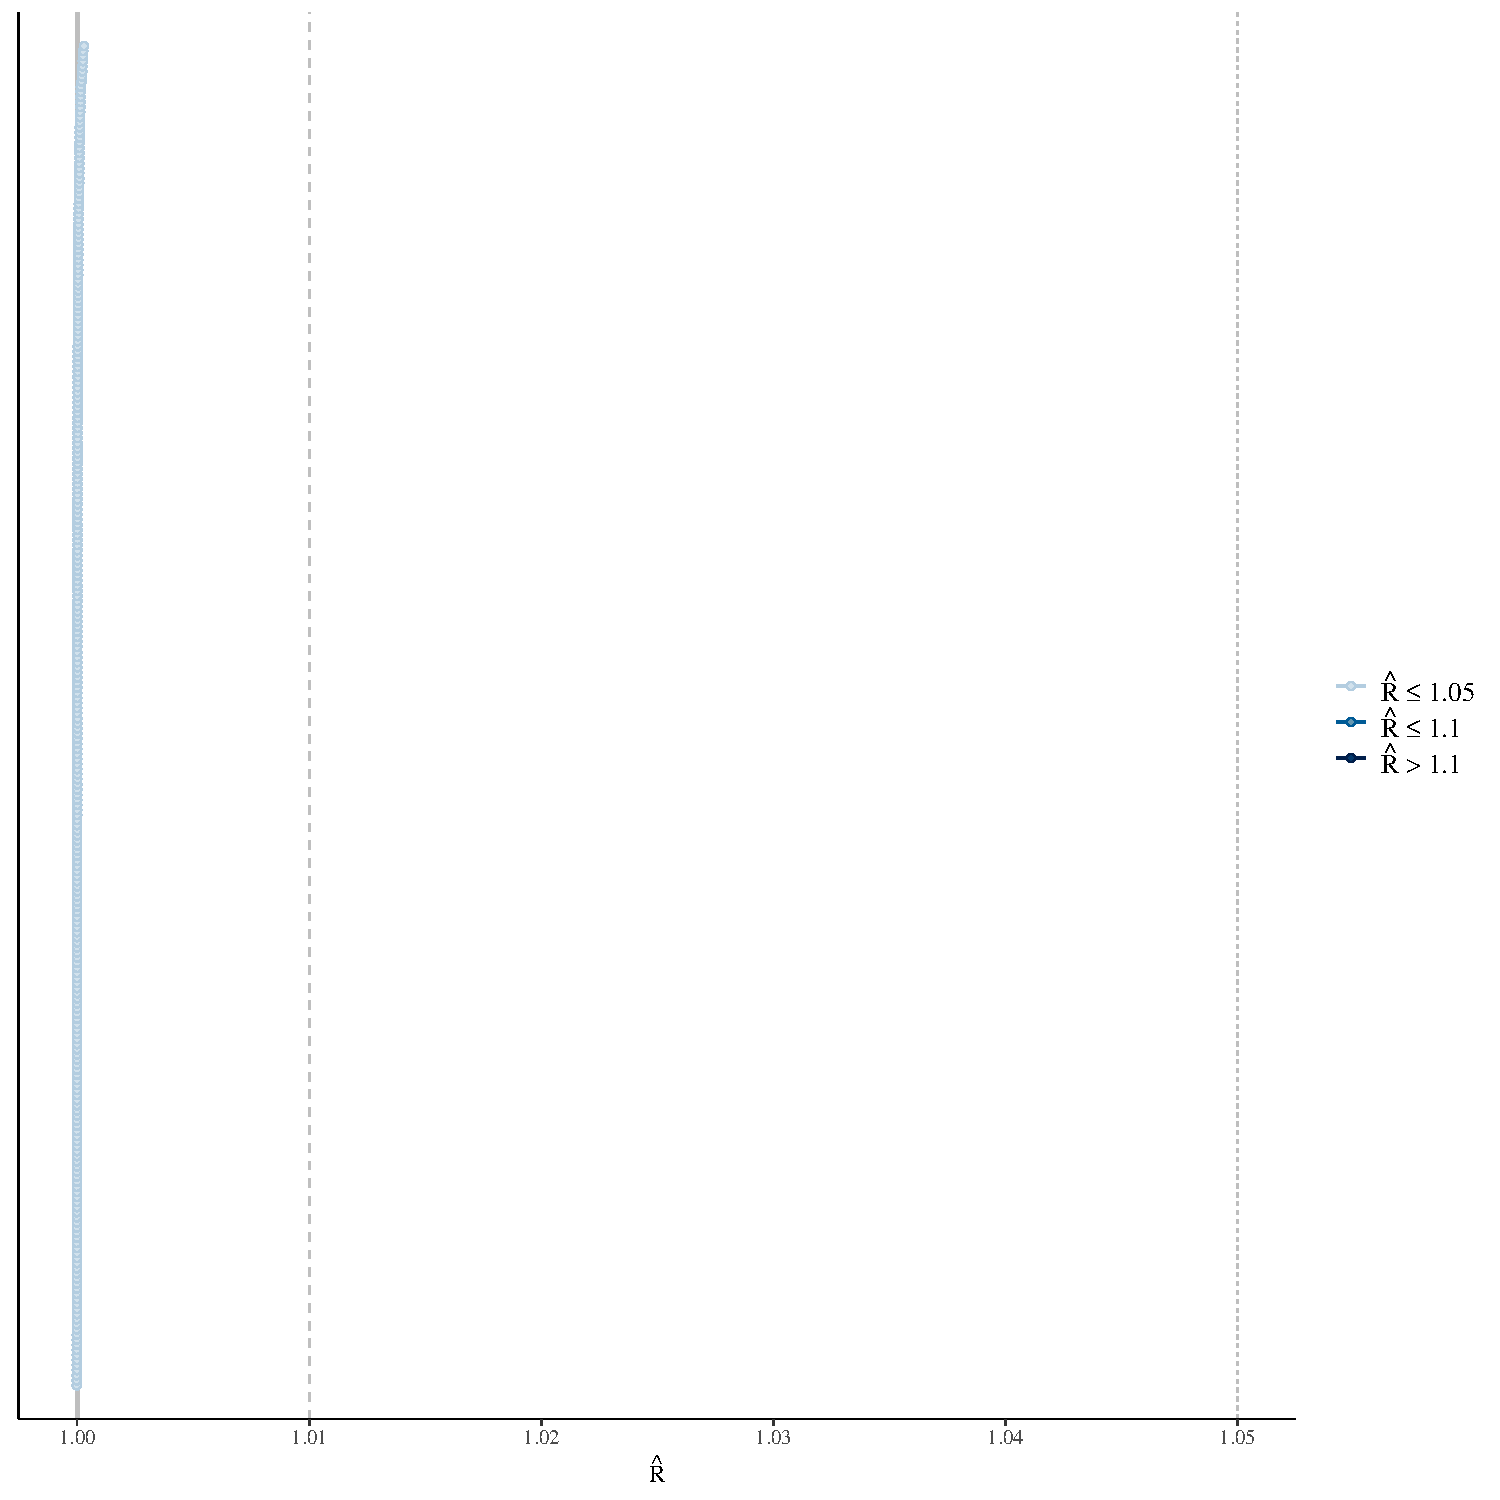
\includegraphics[width=1\textwidth,height=\textheight]{diagnostic_plots_files/figure-pdf/unnamed-chunk-1-1.pdf}

}

\end{figure}

\hypertarget{trace-plots}{%
\section{Trace plots}\label{trace-plots}}

\begin{figure}

{\centering 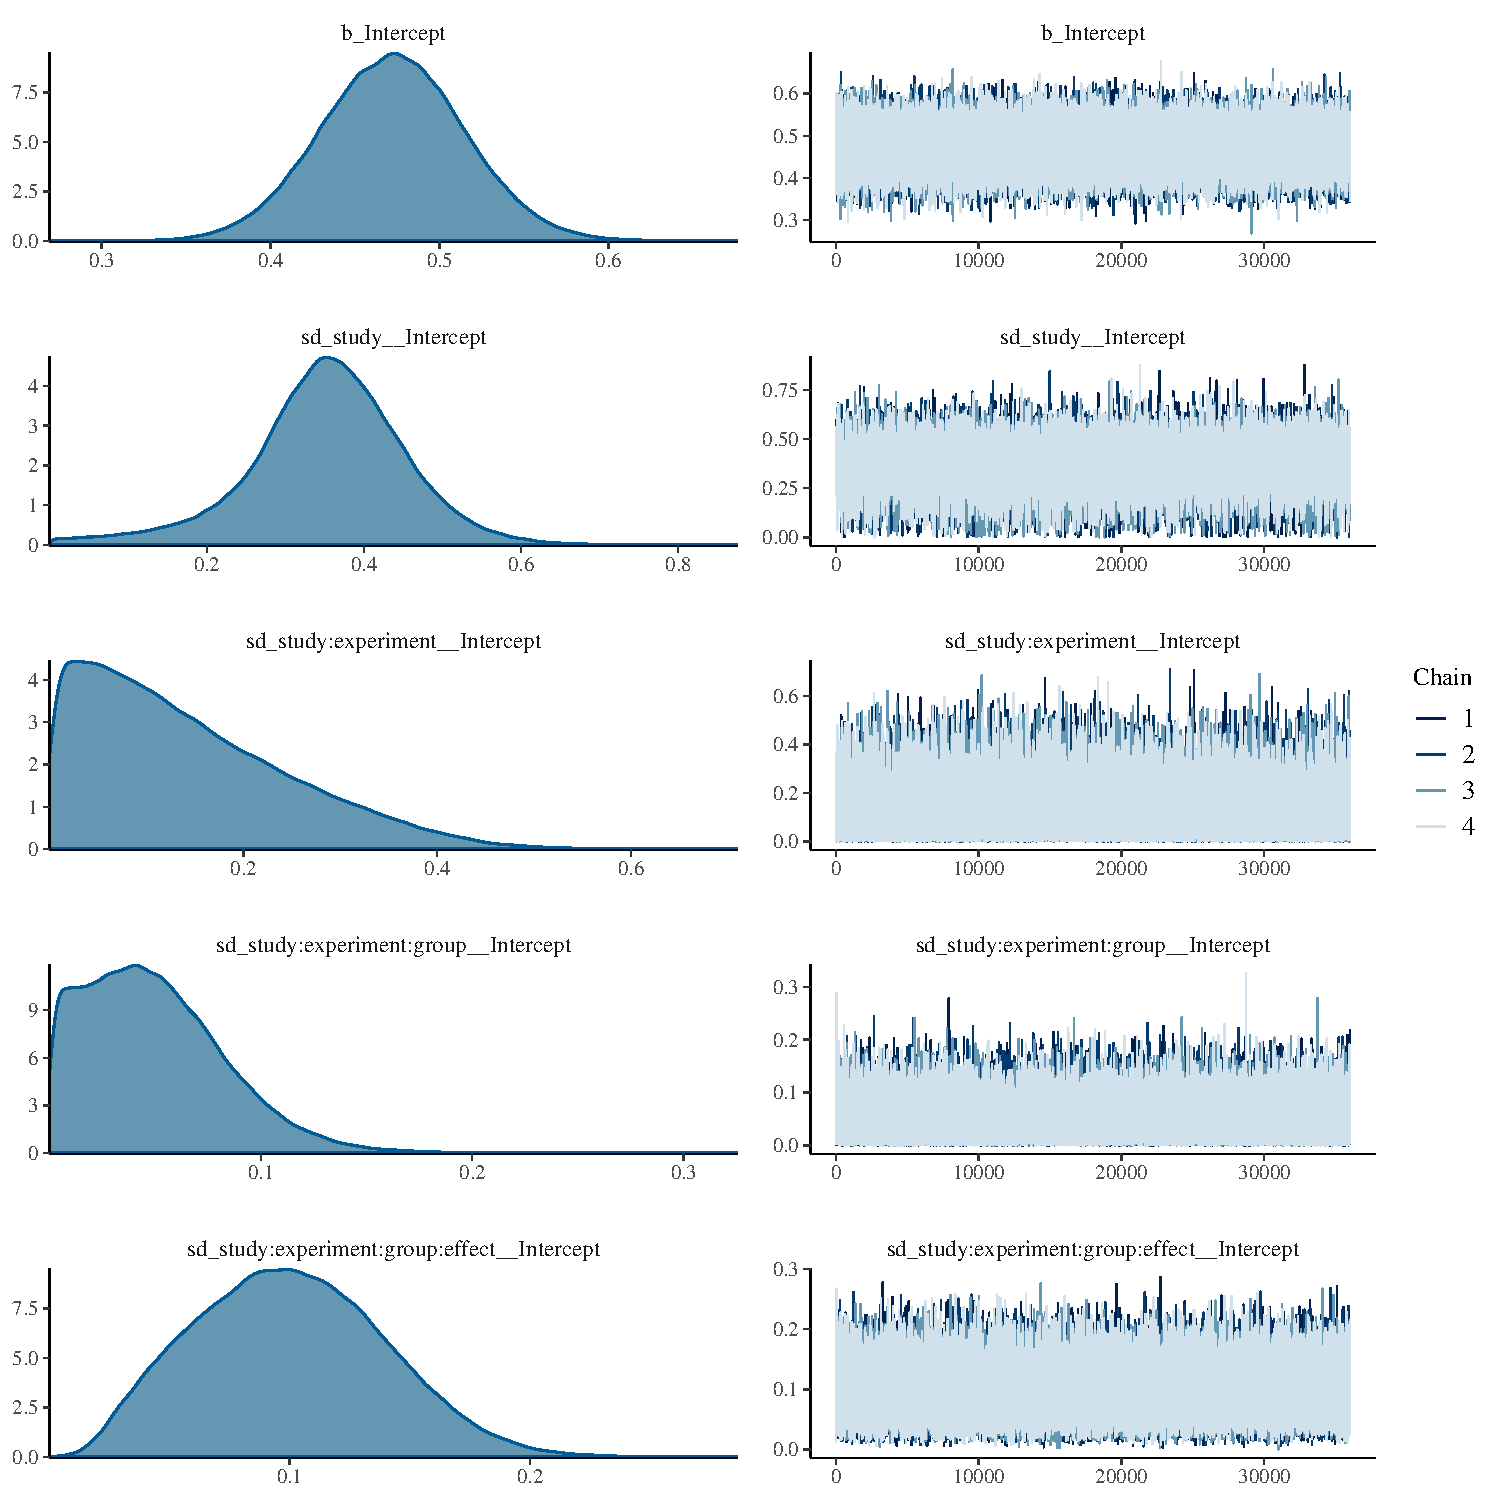
\includegraphics[width=1\textwidth,height=\textheight]{diagnostic_plots_files/figure-pdf/unnamed-chunk-2-1.pdf}

}

\end{figure}

\begin{figure}

{\centering 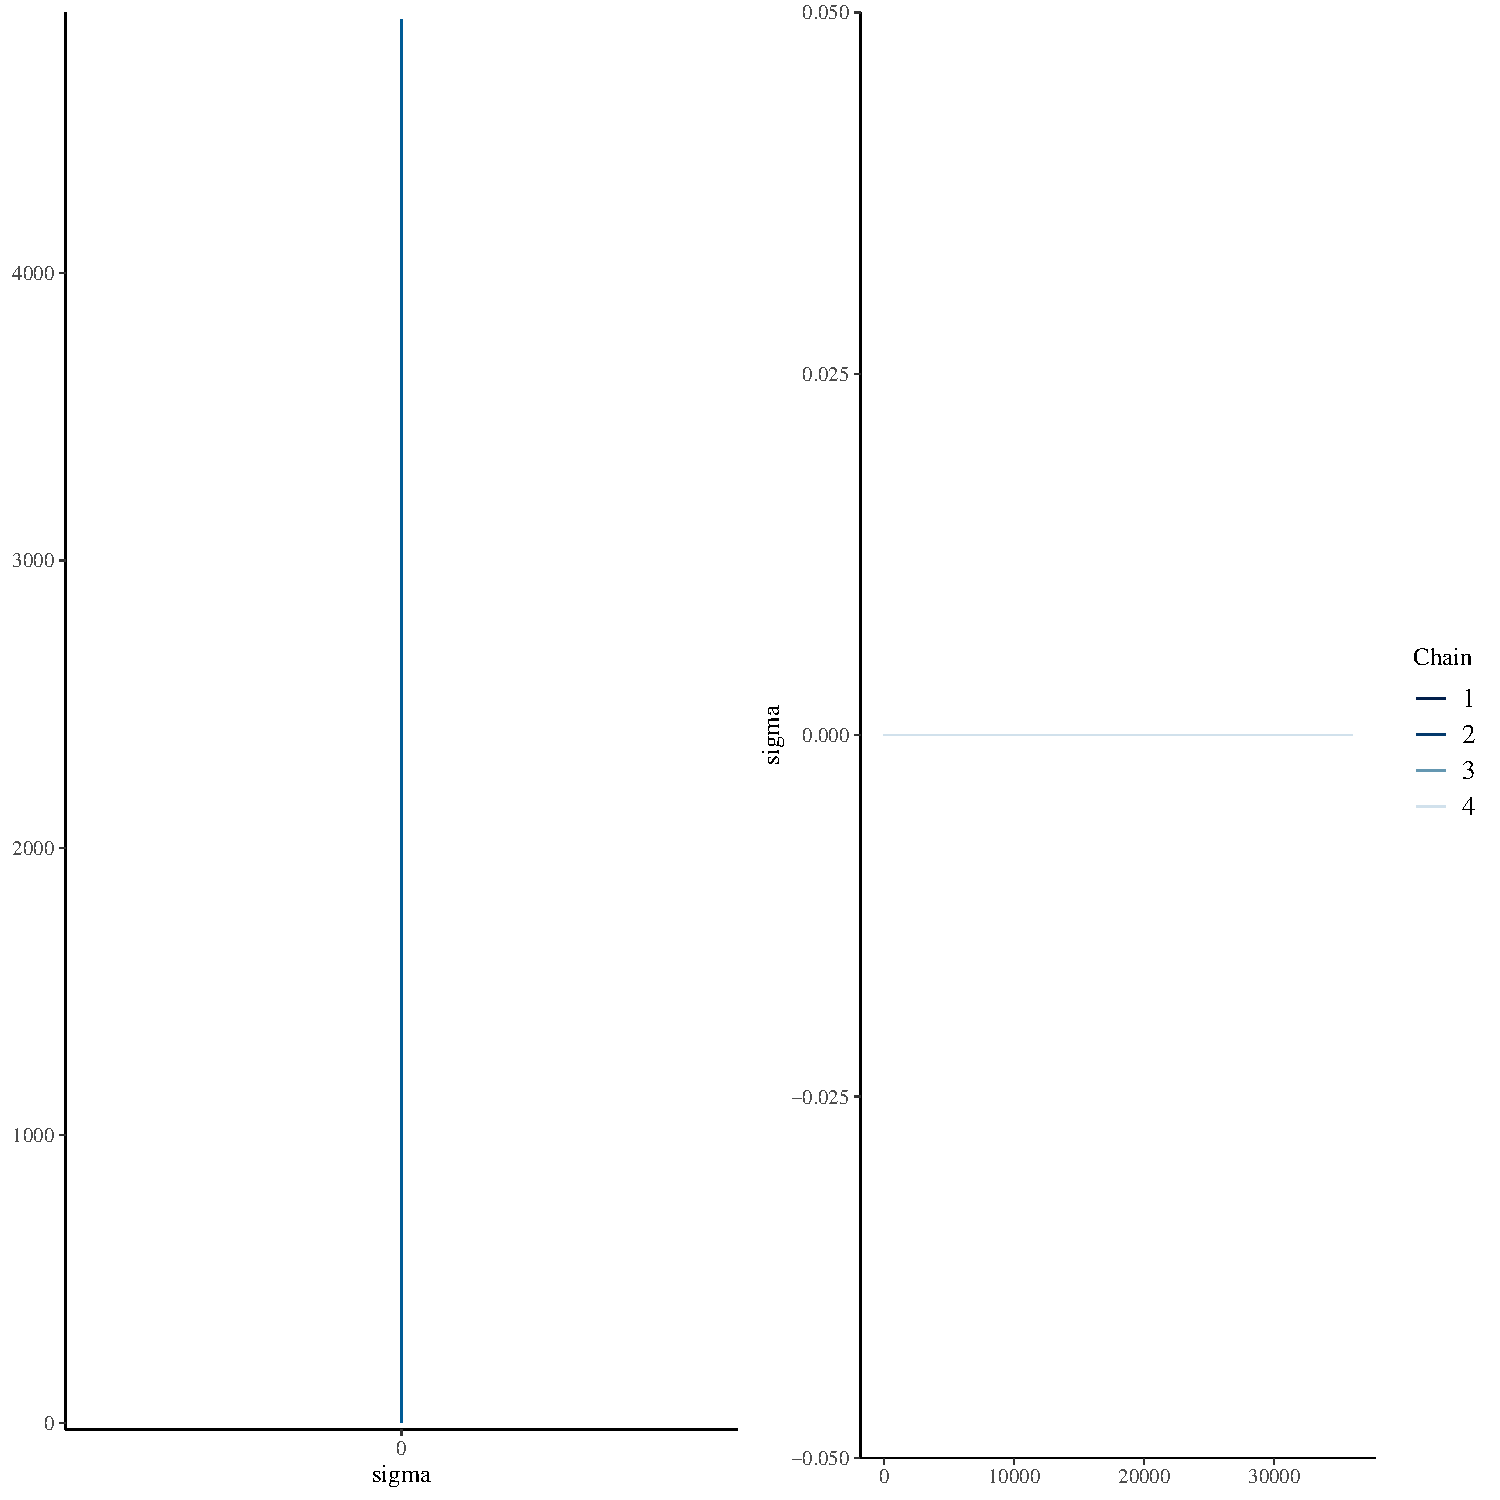
\includegraphics[width=1\textwidth,height=\textheight]{diagnostic_plots_files/figure-pdf/unnamed-chunk-2-2.pdf}

}

\end{figure}

\begin{verbatim}
[[1]]

[[2]]
\end{verbatim}

\hypertarget{posterior-predictive-check}{%
\section{Posterior predictive check}\label{posterior-predictive-check}}

\begin{figure}

{\centering 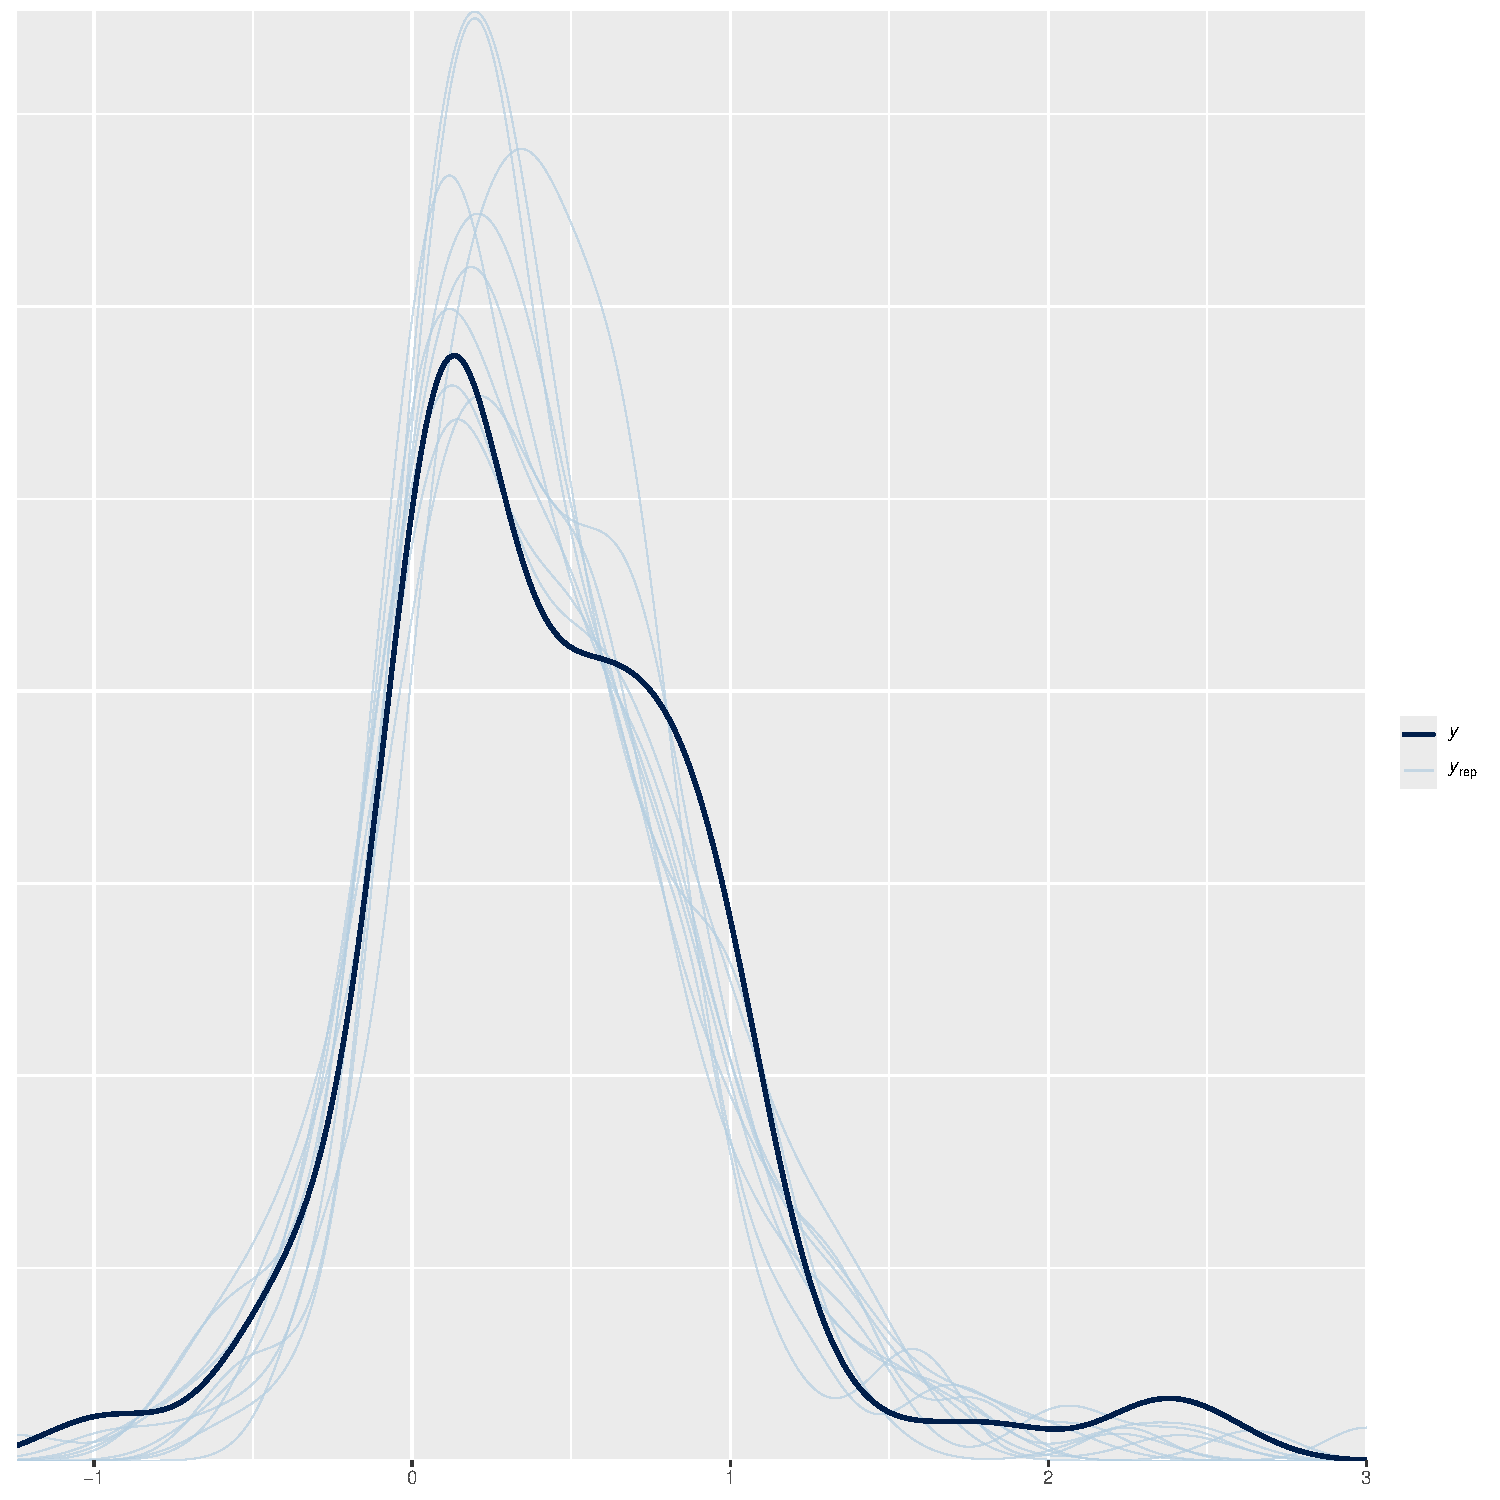
\includegraphics[width=1\textwidth,height=\textheight]{diagnostic_plots_files/figure-pdf/unnamed-chunk-3-1.pdf}

}

\end{figure}

\hypertarget{motor-demands-model}{%
\chapter{Motor Demands Model}\label{motor-demands-model}}

\hypertarget{hatr-1}{%
\section{\texorpdfstring{\(\hat{R}\)}{\textbackslash hat\{R\}}}\label{hatr-1}}

\begin{figure}

{\centering 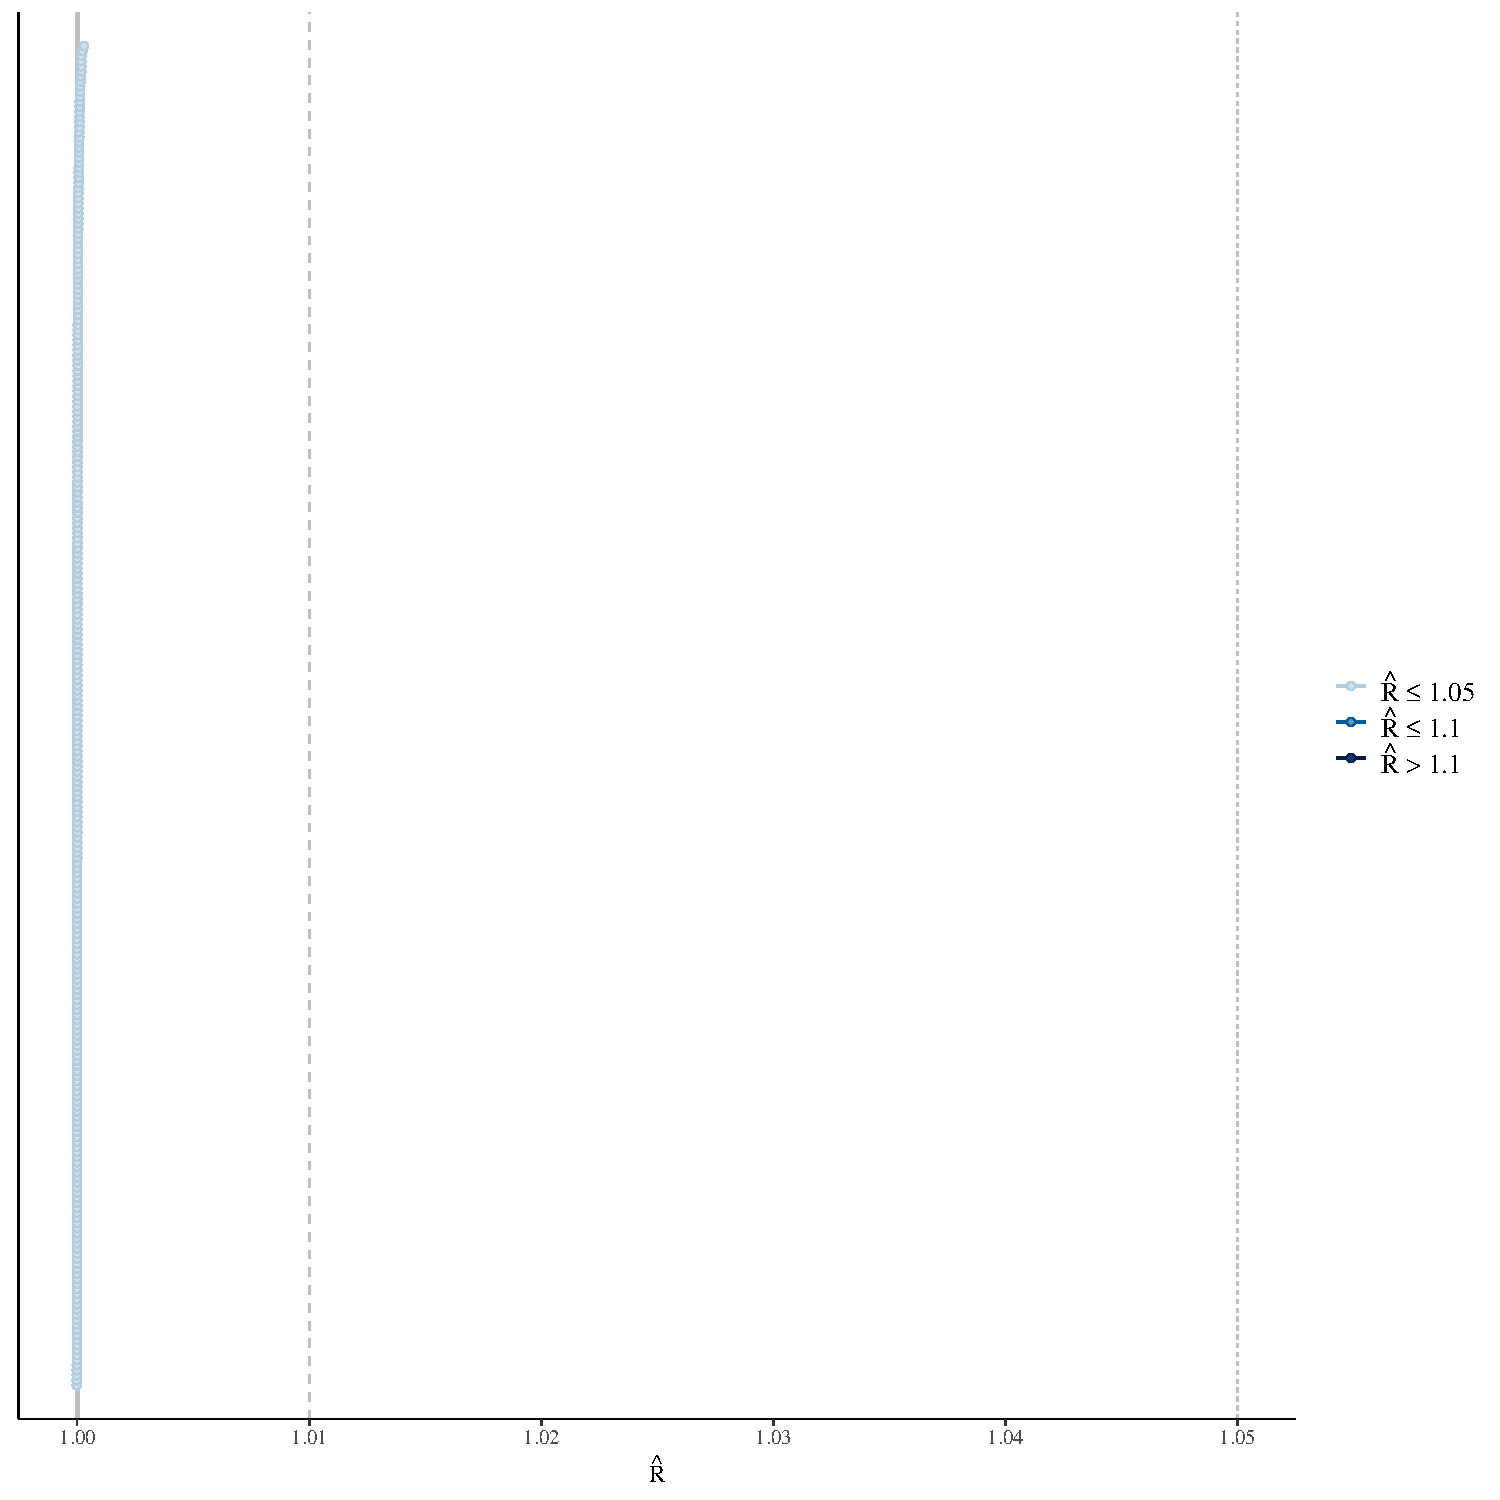
\includegraphics[width=1\textwidth,height=\textheight]{diagnostic_plots_files/figure-pdf/unnamed-chunk-4-1.pdf}

}

\end{figure}

\hypertarget{trace-plots-1}{%
\section{Trace plots}\label{trace-plots-1}}

\begin{figure}

{\centering 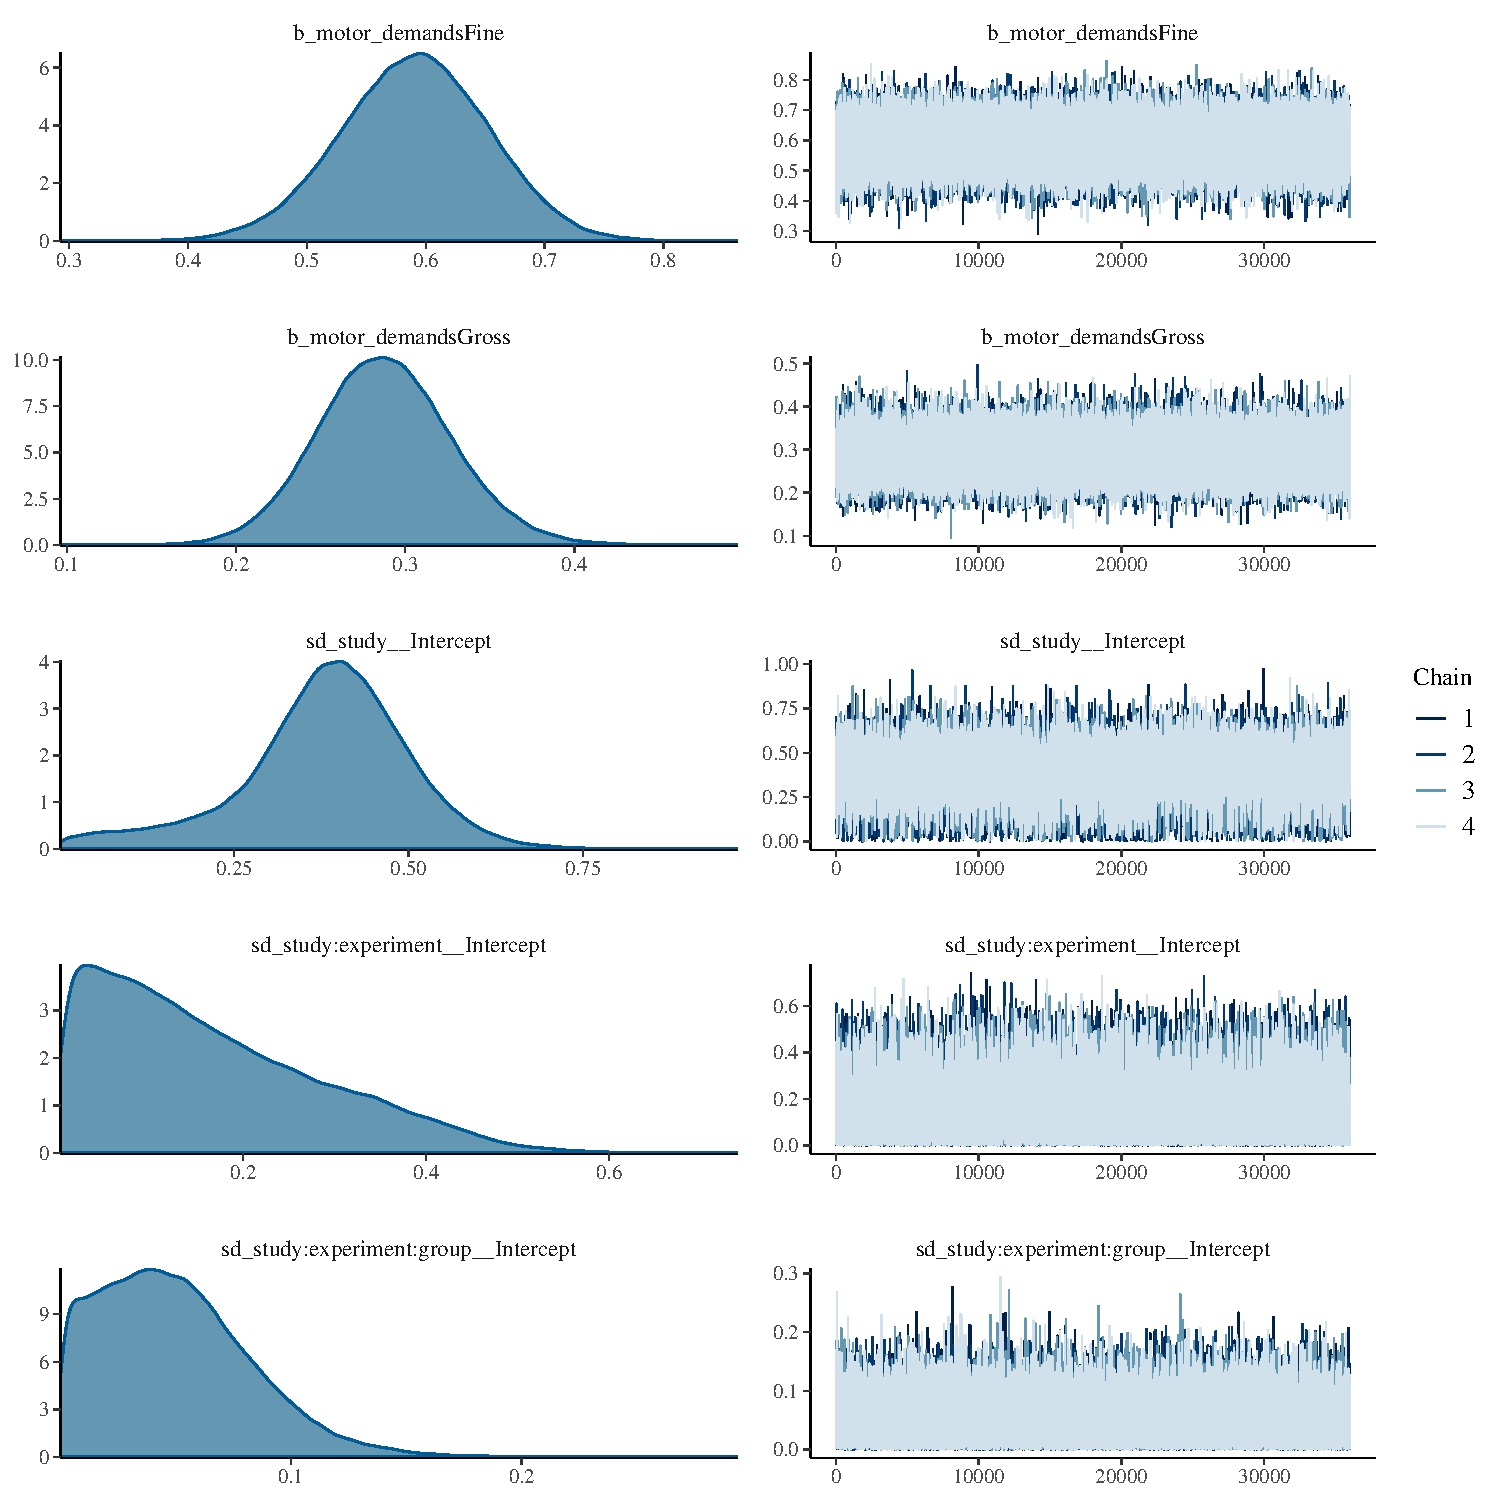
\includegraphics[width=1\textwidth,height=\textheight]{diagnostic_plots_files/figure-pdf/unnamed-chunk-5-1.pdf}

}

\end{figure}

\begin{figure}

{\centering 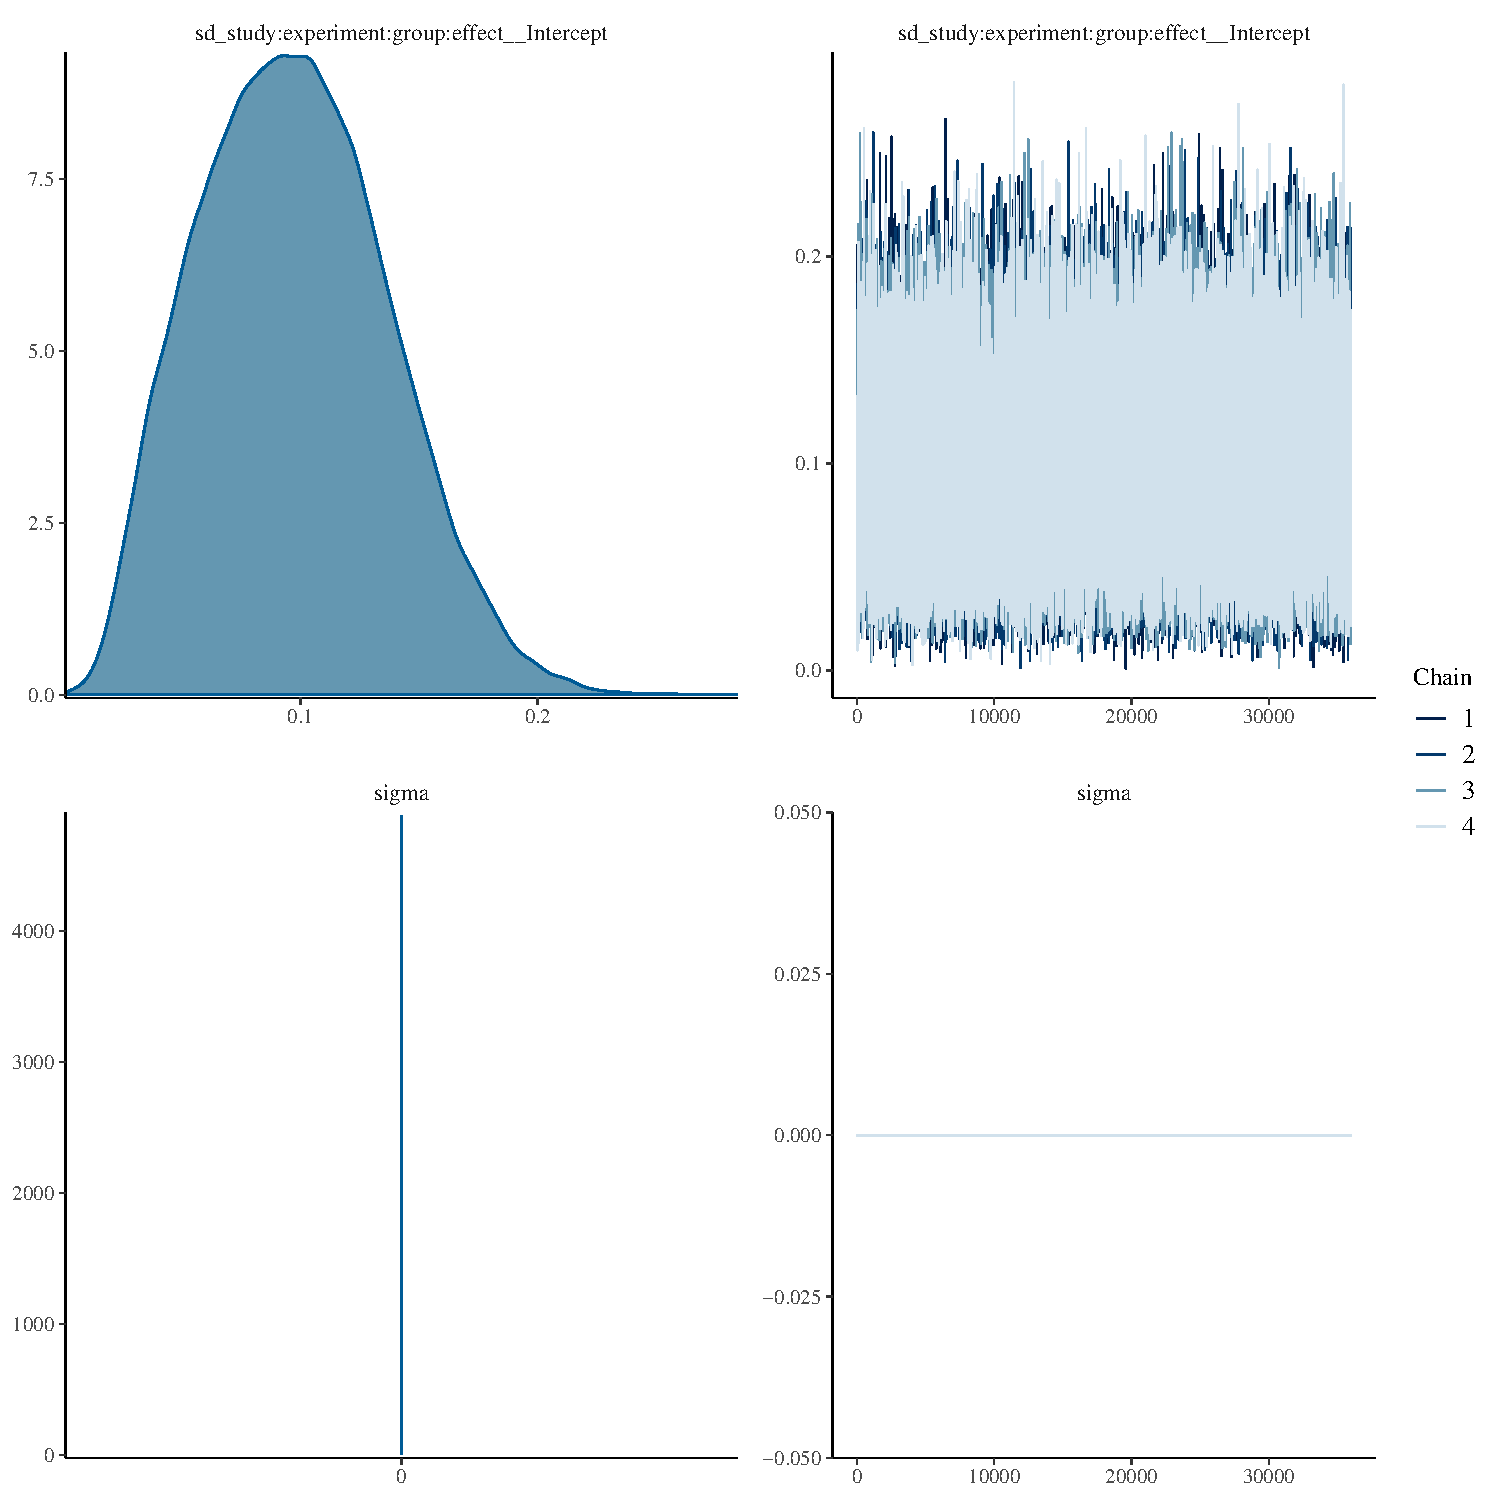
\includegraphics[width=1\textwidth,height=\textheight]{diagnostic_plots_files/figure-pdf/unnamed-chunk-5-2.pdf}

}

\end{figure}

\begin{verbatim}
[[1]]

[[2]]
\end{verbatim}

\hypertarget{posterior-predictive-check-1}{%
\section{Posterior predictive
check}\label{posterior-predictive-check-1}}

\begin{figure}

{\centering 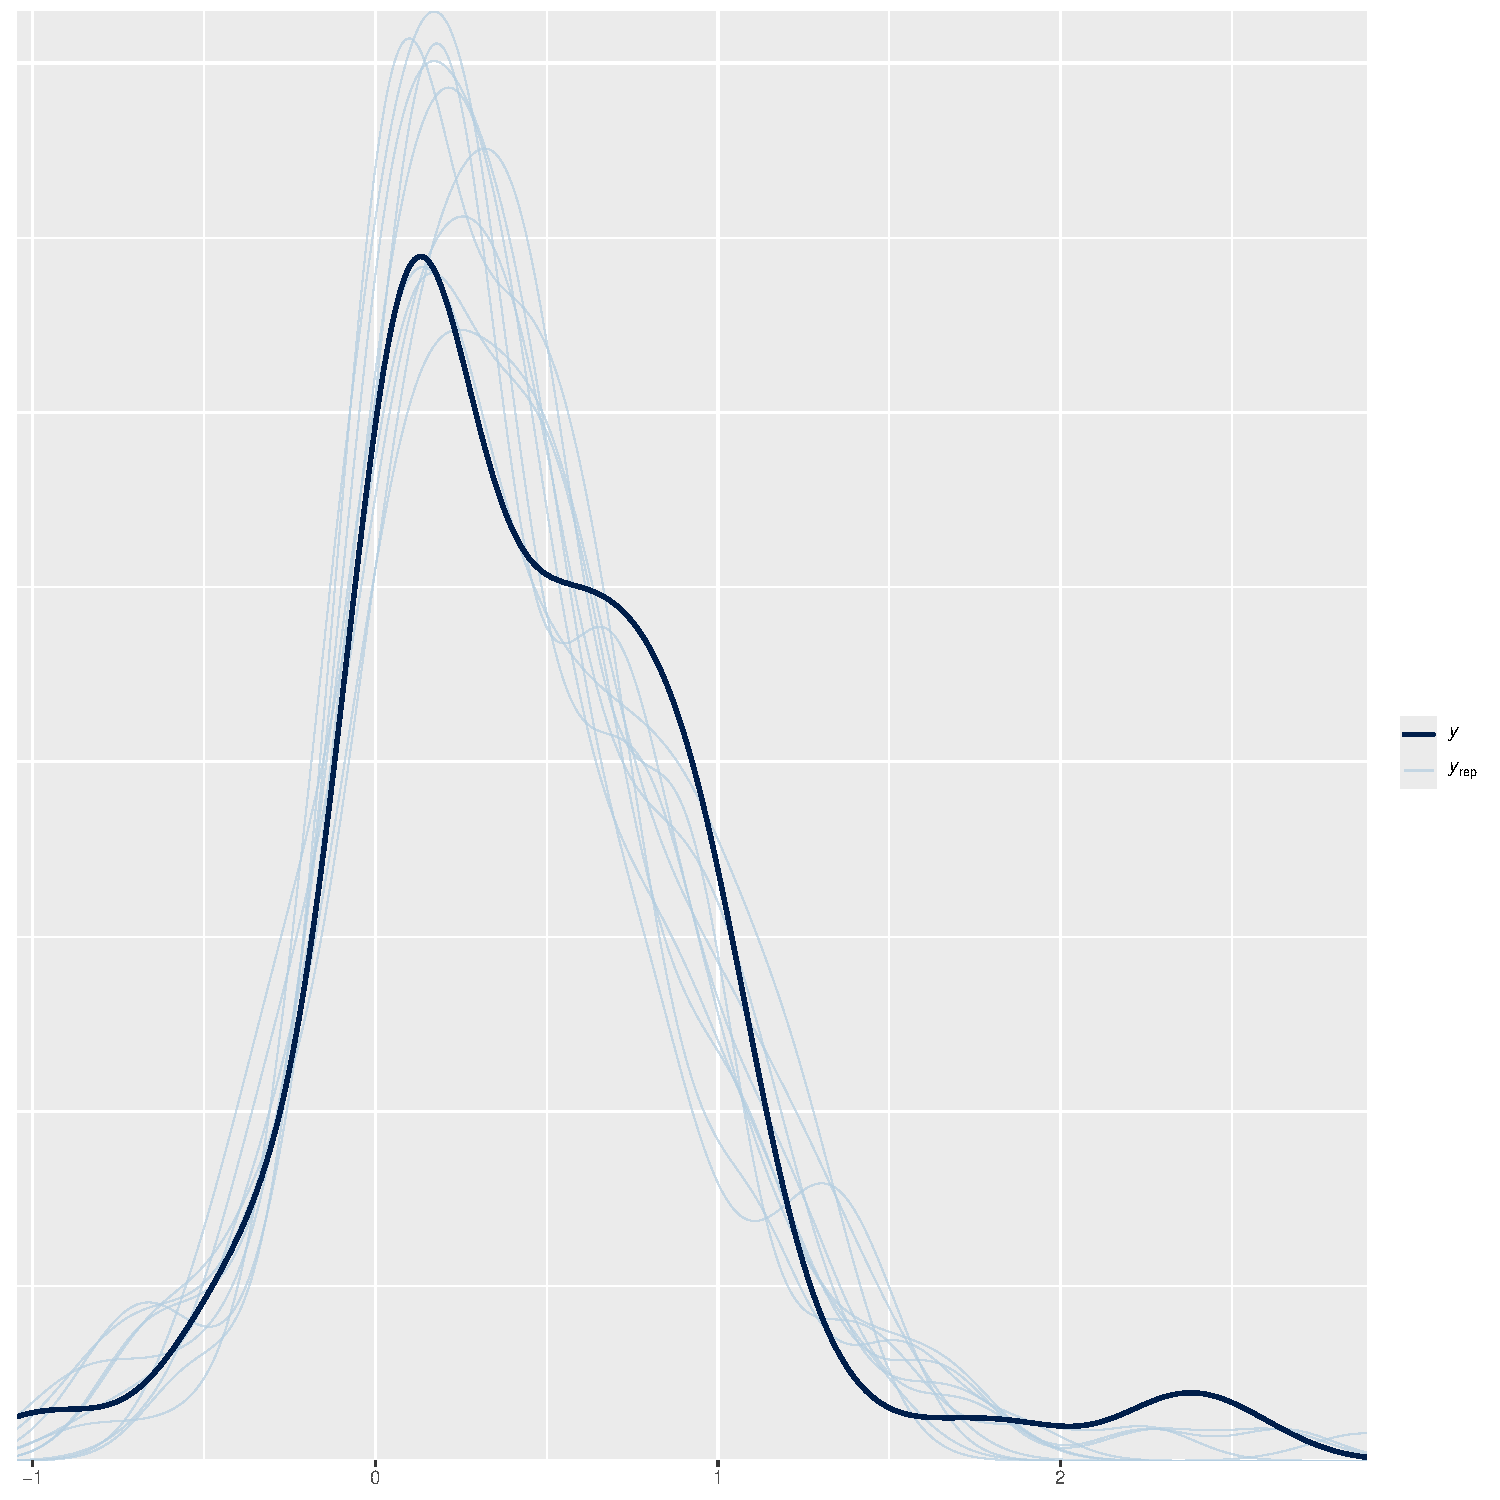
\includegraphics[width=1\textwidth,height=\textheight]{diagnostic_plots_files/figure-pdf/unnamed-chunk-6-1.pdf}

}

\end{figure}

\hypertarget{participant-group-model}{%
\chapter{Participant Group Model}\label{participant-group-model}}

\hypertarget{hatr-2}{%
\section{\texorpdfstring{\(\hat{R}\)}{\textbackslash hat\{R\}}}\label{hatr-2}}

\begin{figure}

{\centering 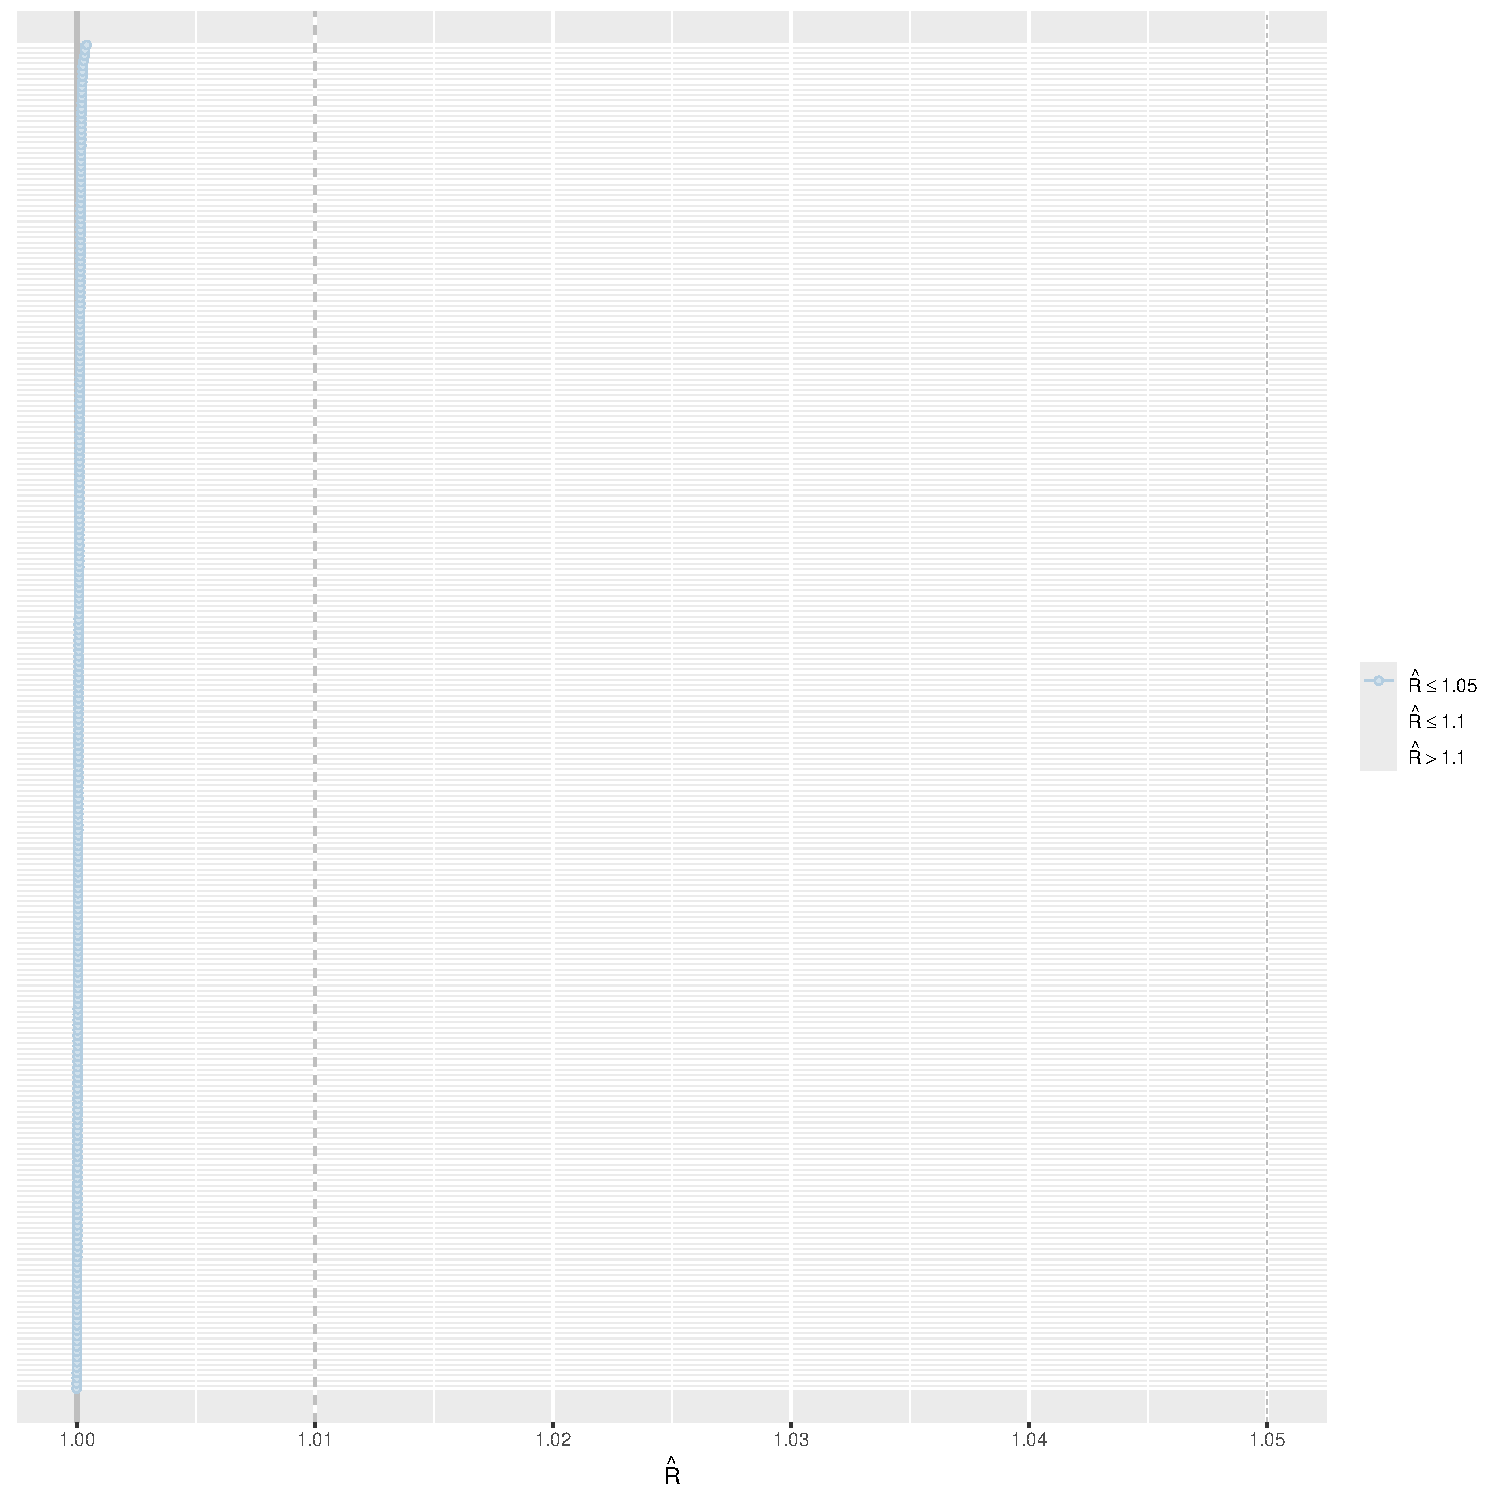
\includegraphics[width=1\textwidth,height=\textheight]{diagnostic_plots_files/figure-pdf/unnamed-chunk-7-1.pdf}

}

\end{figure}

\hypertarget{trace-plots-2}{%
\section{Trace plots}\label{trace-plots-2}}

\begin{figure}

{\centering 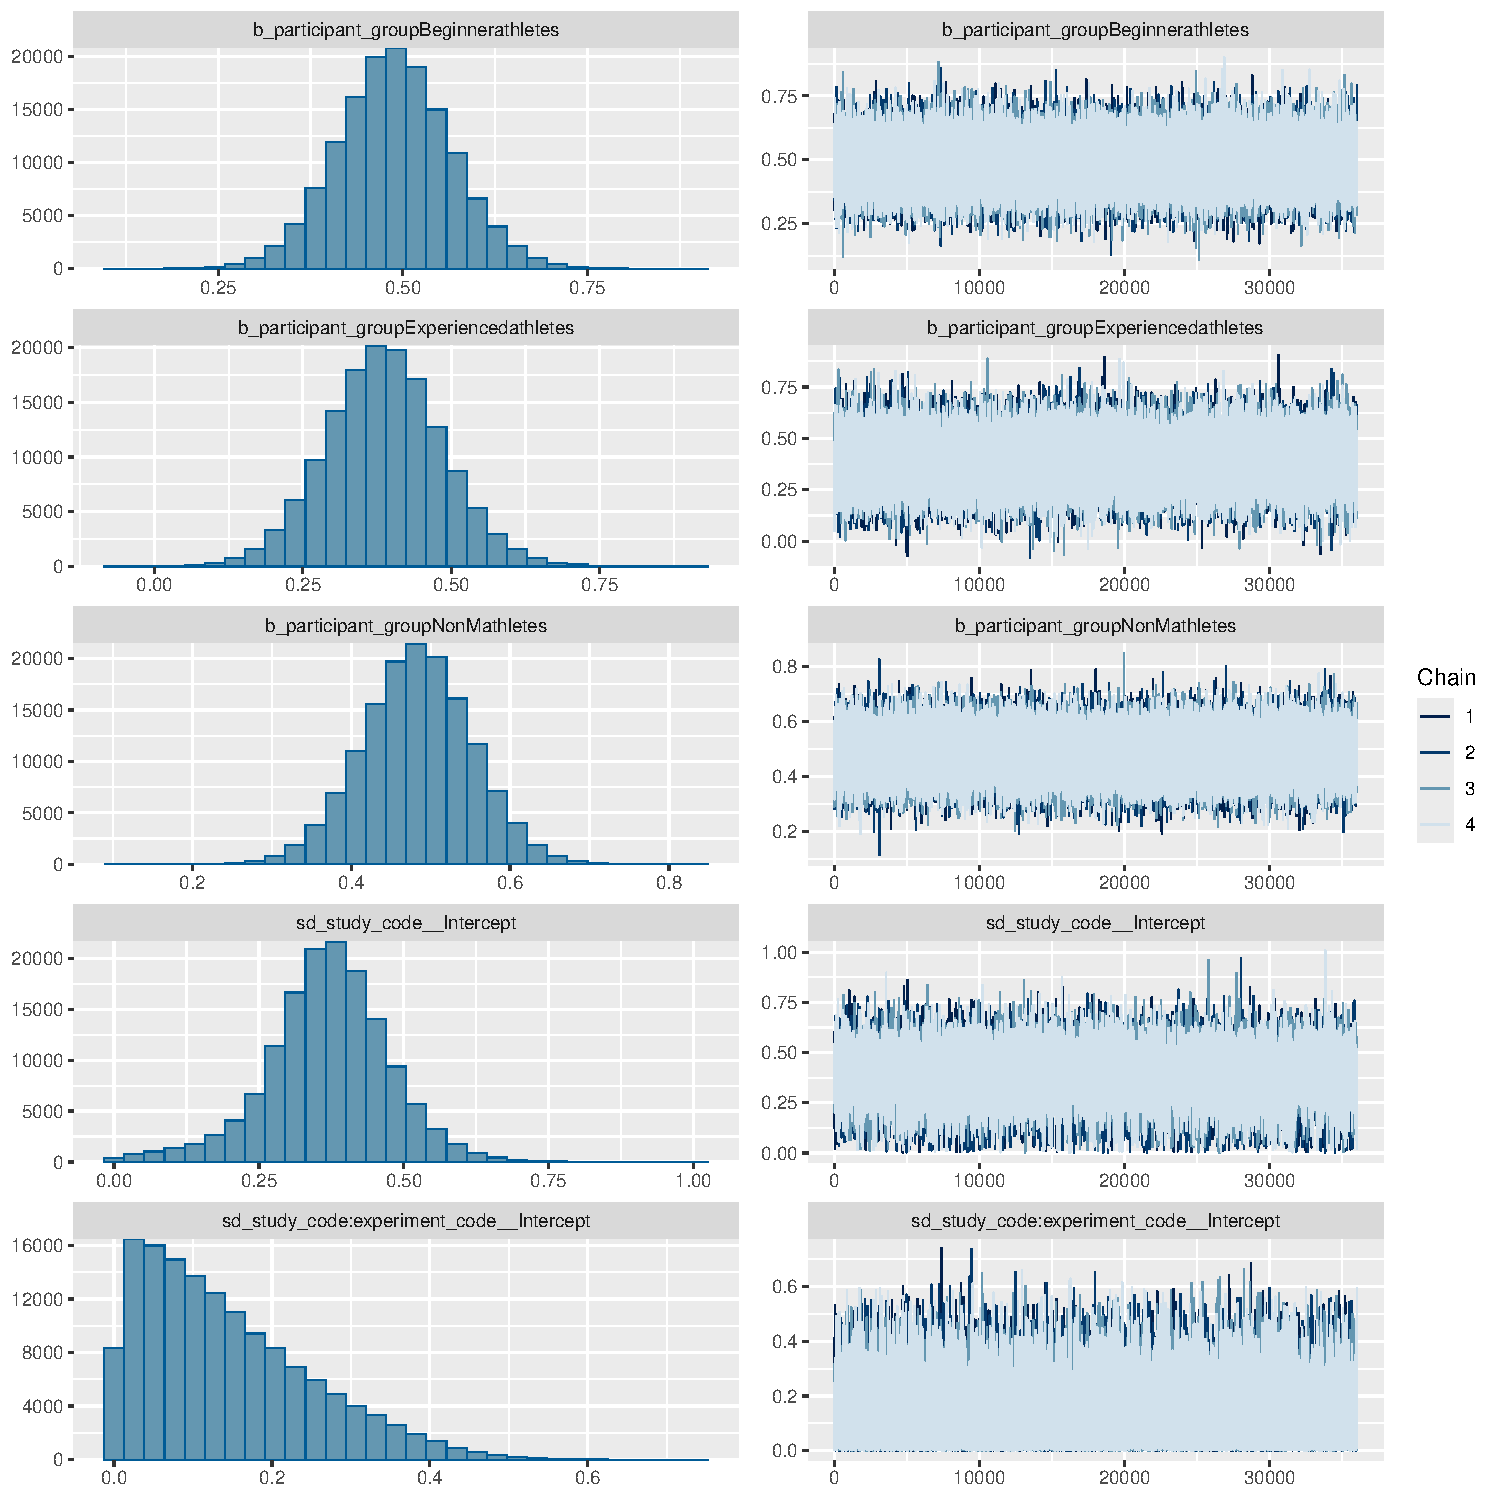
\includegraphics[width=1\textwidth,height=\textheight]{diagnostic_plots_files/figure-pdf/unnamed-chunk-8-1.pdf}

}

\end{figure}

\begin{figure}

{\centering 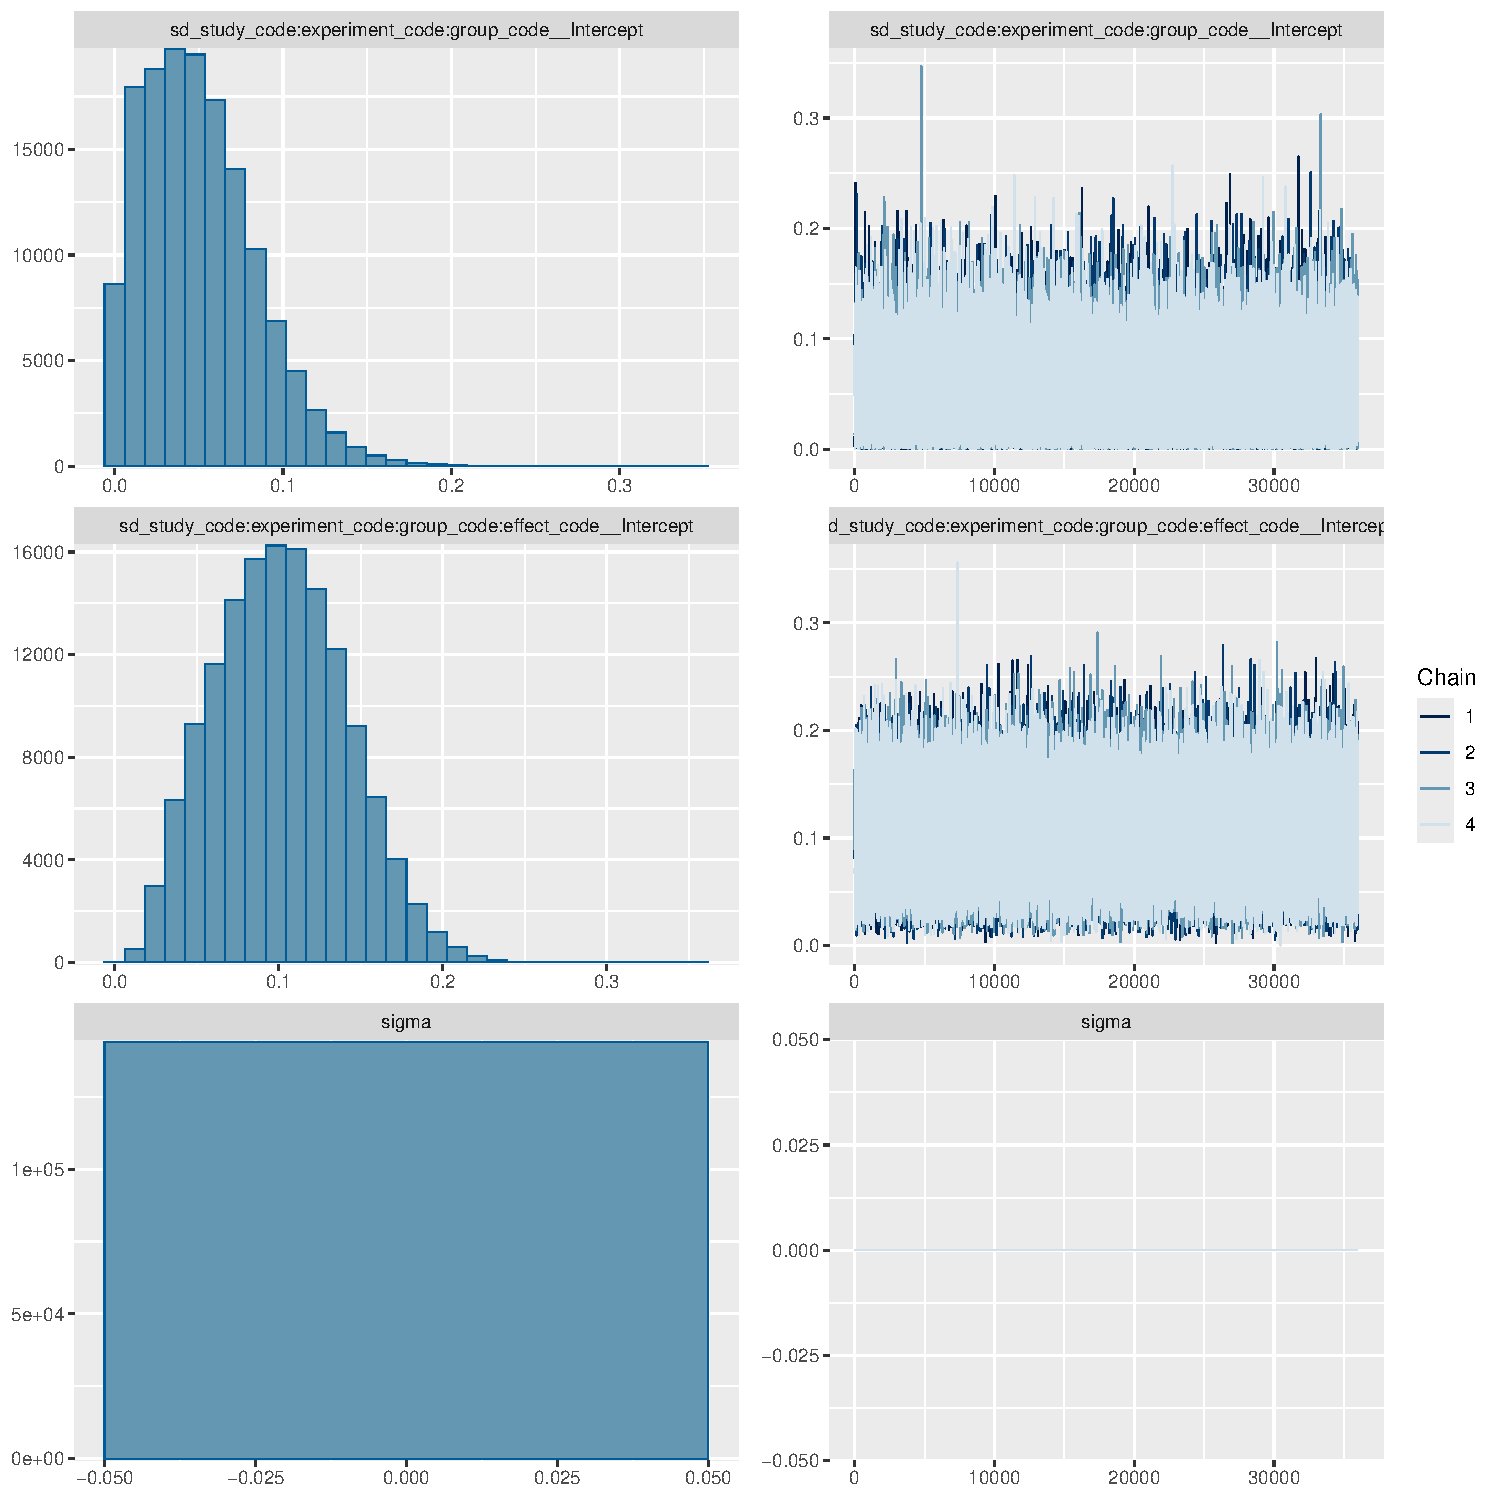
\includegraphics[width=1\textwidth,height=\textheight]{diagnostic_plots_files/figure-pdf/unnamed-chunk-8-2.pdf}

}

\end{figure}

\begin{verbatim}
[[1]]

[[2]]
\end{verbatim}

\hypertarget{posterior-predictive-check-2}{%
\section{Posterior predictive
check}\label{posterior-predictive-check-2}}

\begin{figure}

{\centering 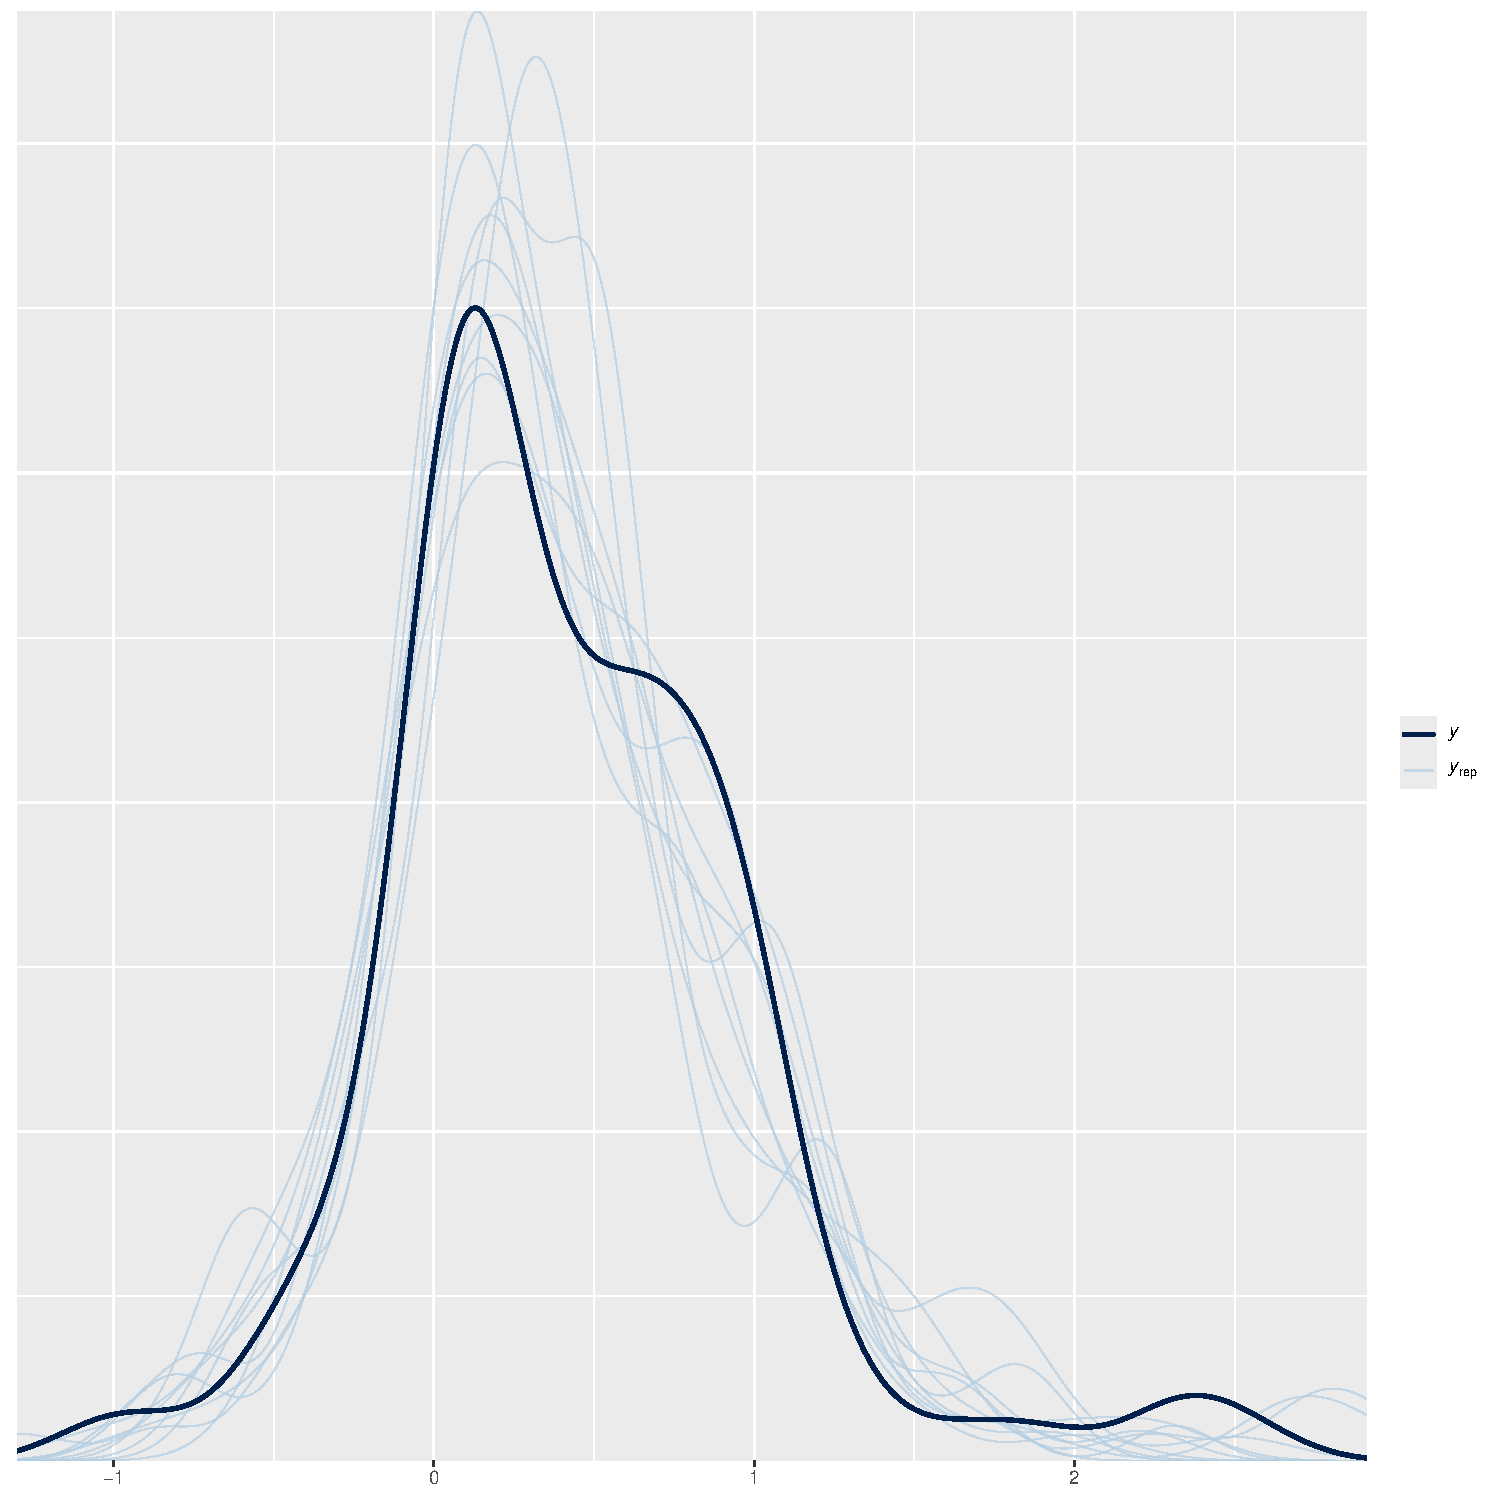
\includegraphics[width=1\textwidth,height=\textheight]{diagnostic_plots_files/figure-pdf/unnamed-chunk-9-1.pdf}

}

\end{figure}

\hypertarget{self-talk-content-model}{%
\chapter{Self-Talk Content Model}\label{self-talk-content-model}}

\hypertarget{hatr-3}{%
\section{\texorpdfstring{\(\hat{R}\)}{\textbackslash hat\{R\}}}\label{hatr-3}}

\begin{figure}

{\centering 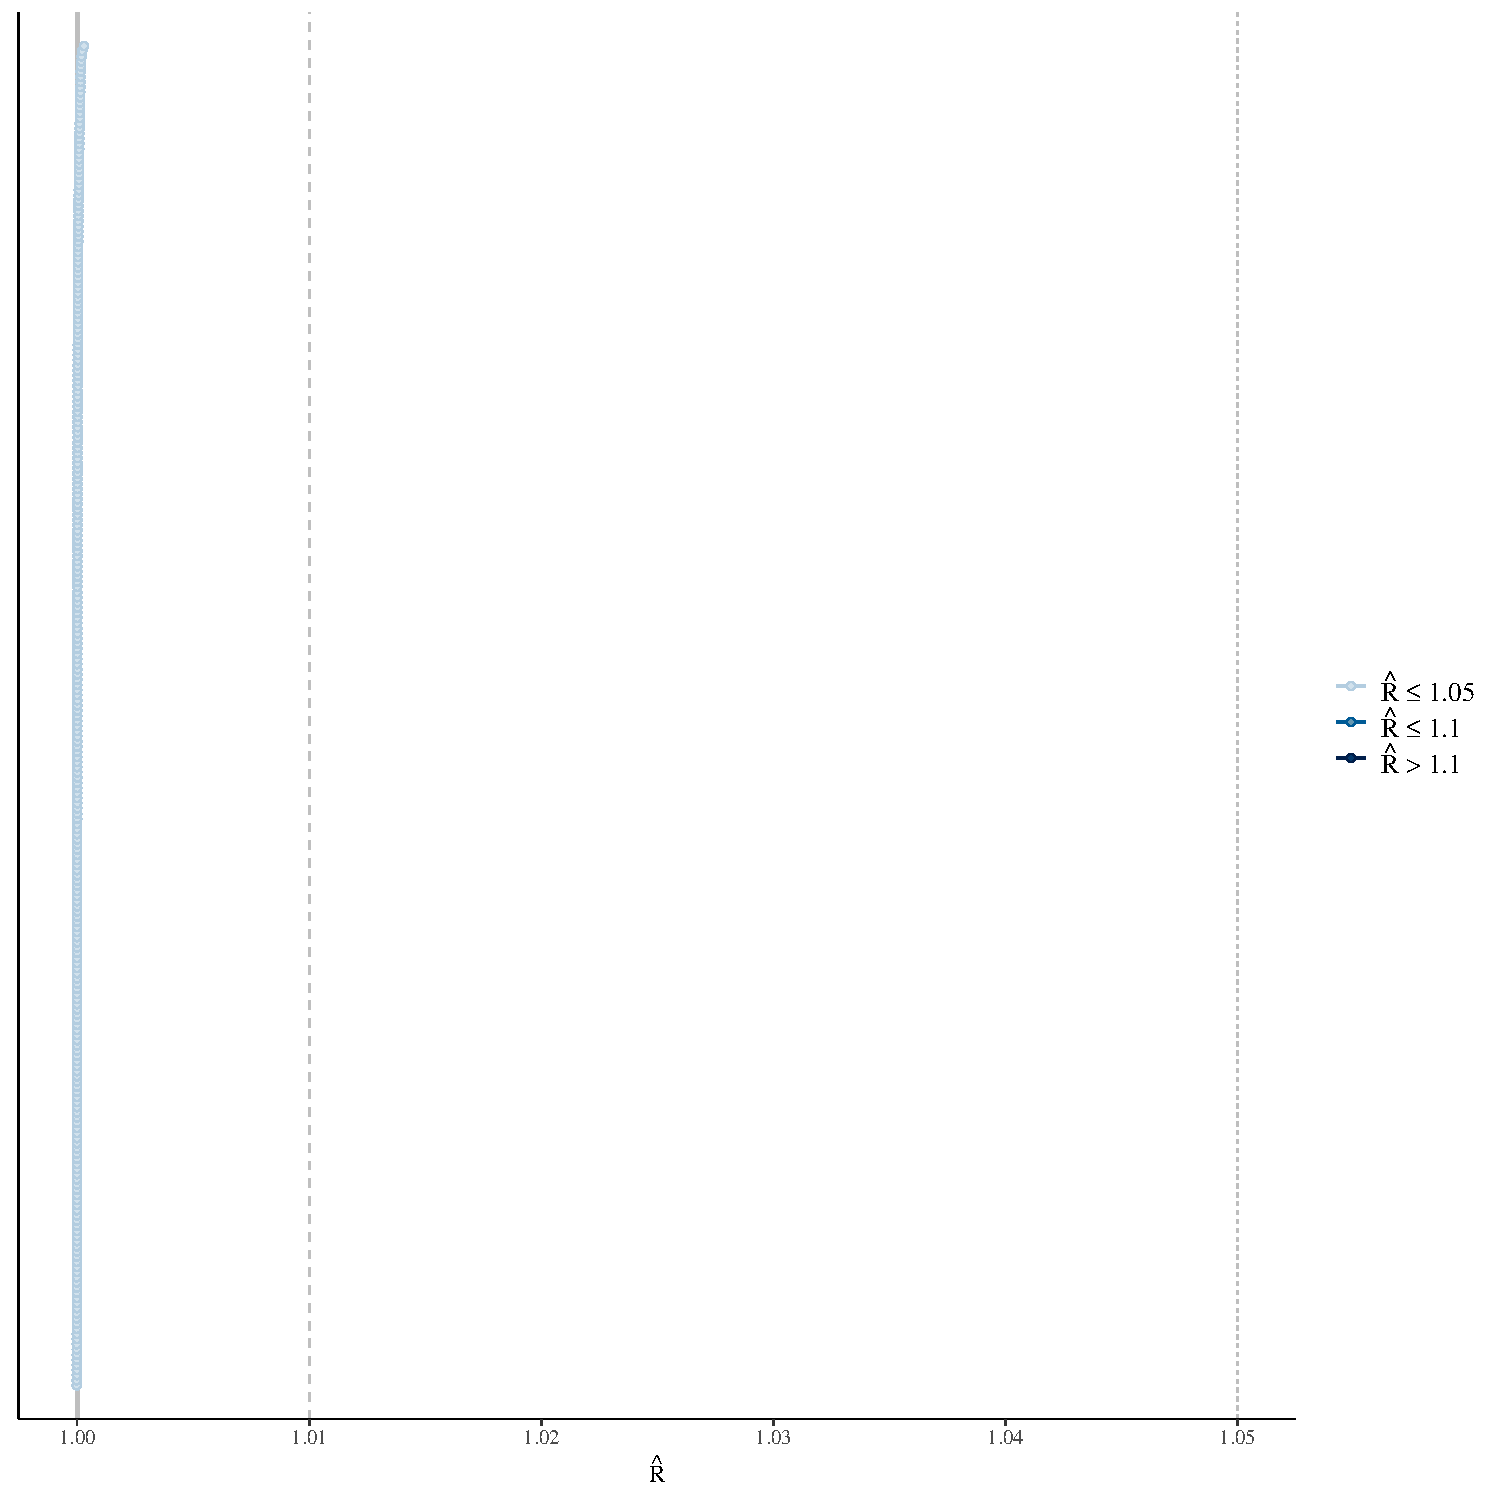
\includegraphics[width=1\textwidth,height=\textheight]{diagnostic_plots_files/figure-pdf/unnamed-chunk-10-1.pdf}

}

\end{figure}

\hypertarget{trace-plots-3}{%
\section{Trace plots}\label{trace-plots-3}}

\begin{figure}

{\centering 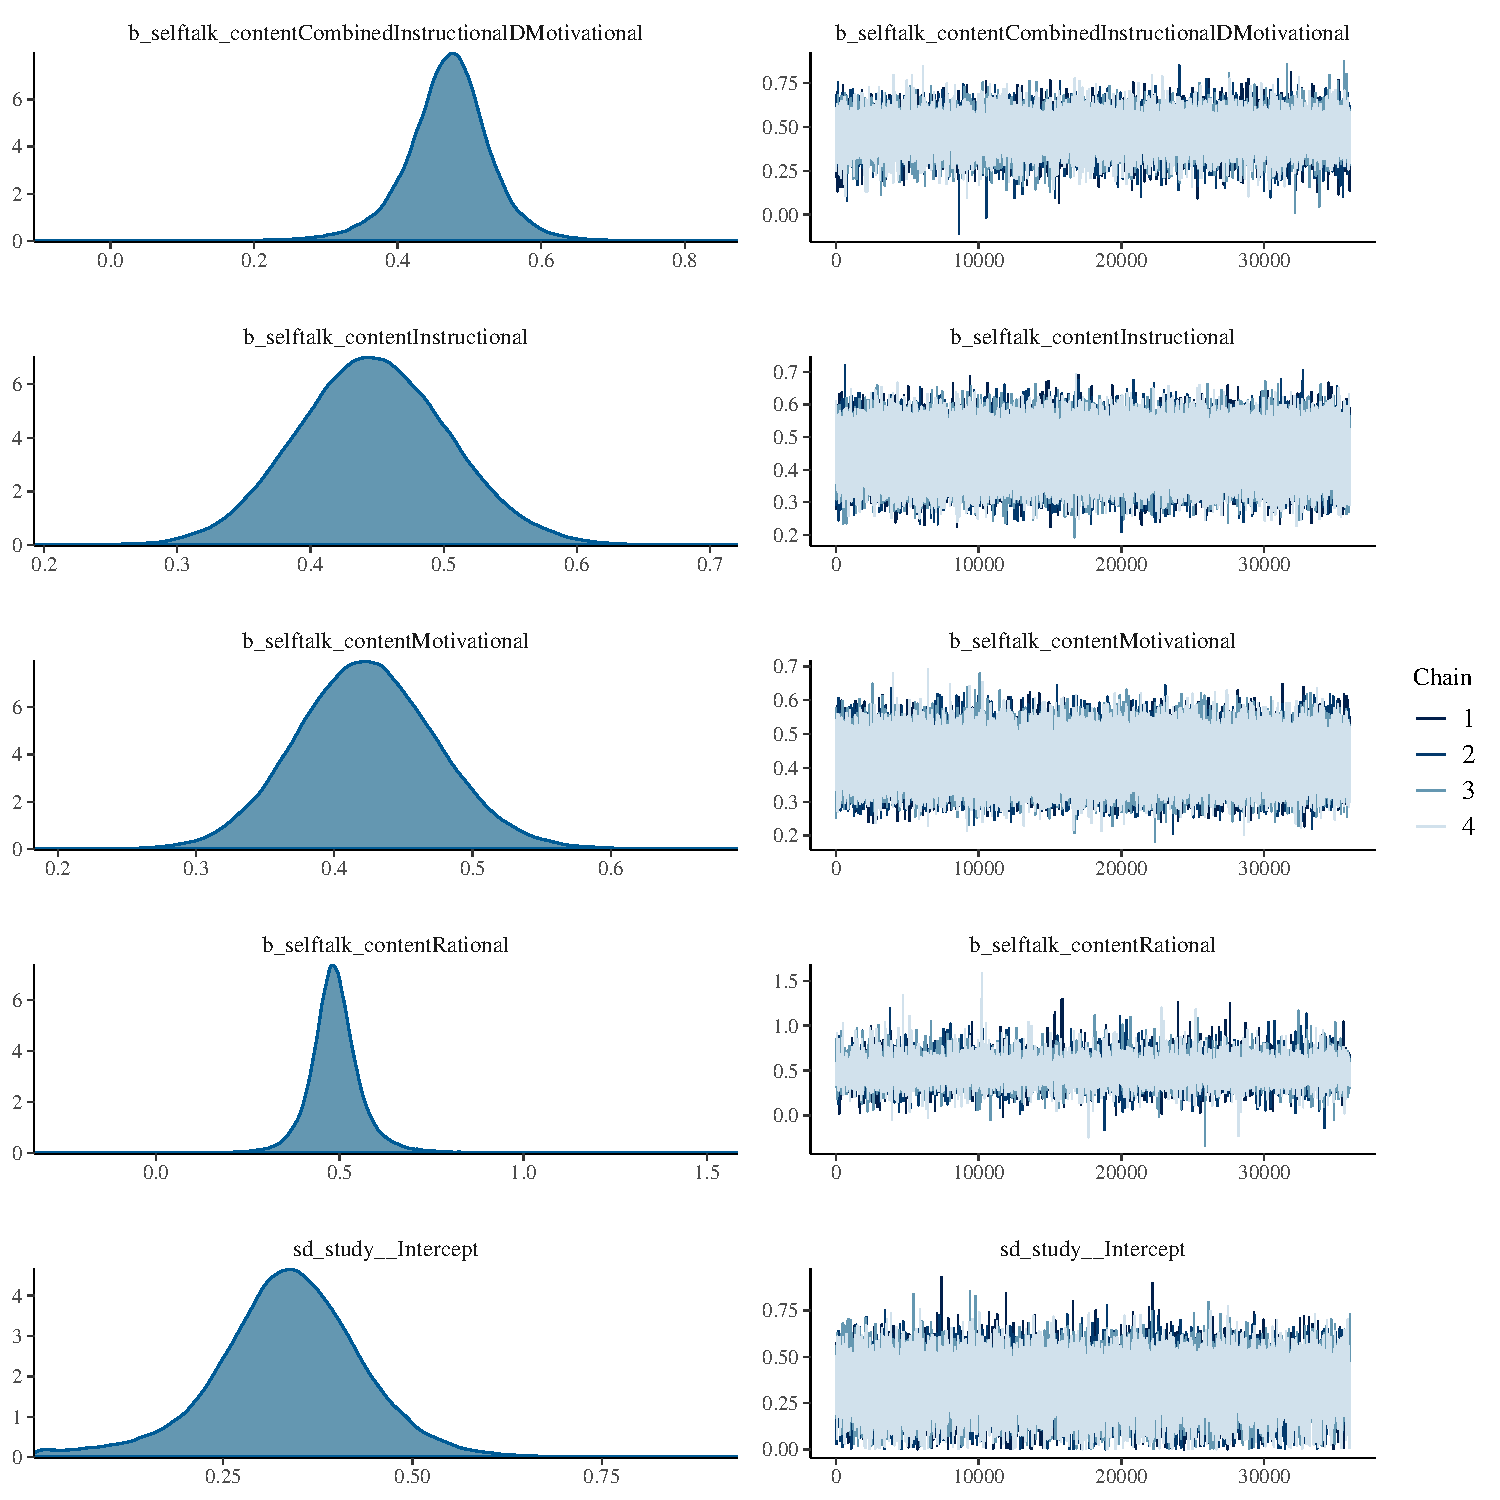
\includegraphics[width=1\textwidth,height=\textheight]{diagnostic_plots_files/figure-pdf/unnamed-chunk-11-1.pdf}

}

\end{figure}

\begin{figure}

{\centering 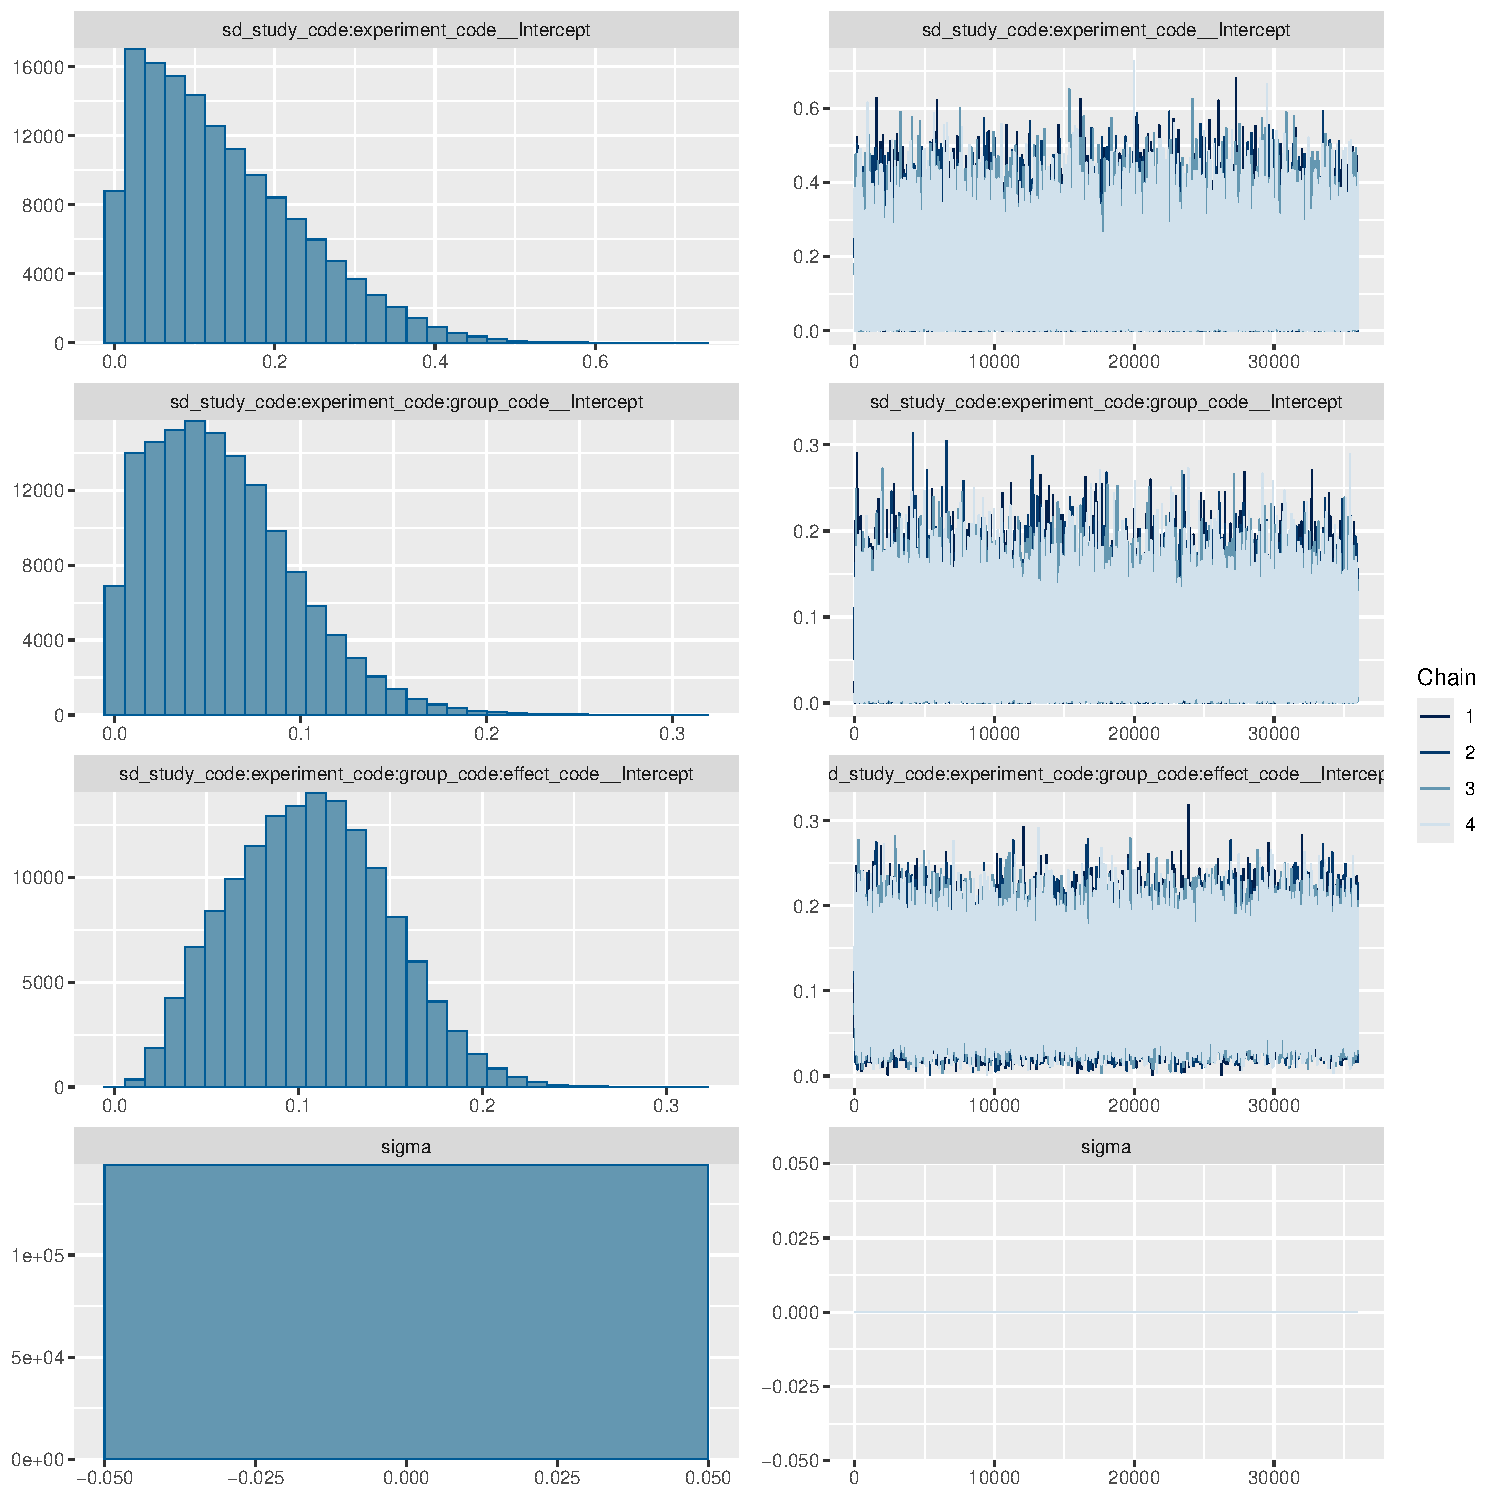
\includegraphics[width=1\textwidth,height=\textheight]{diagnostic_plots_files/figure-pdf/unnamed-chunk-11-2.pdf}

}

\end{figure}

\begin{verbatim}
[[1]]

[[2]]
\end{verbatim}

\hypertarget{posterior-predictive-check-3}{%
\section{Posterior predictive
check}\label{posterior-predictive-check-3}}

\begin{figure}

{\centering 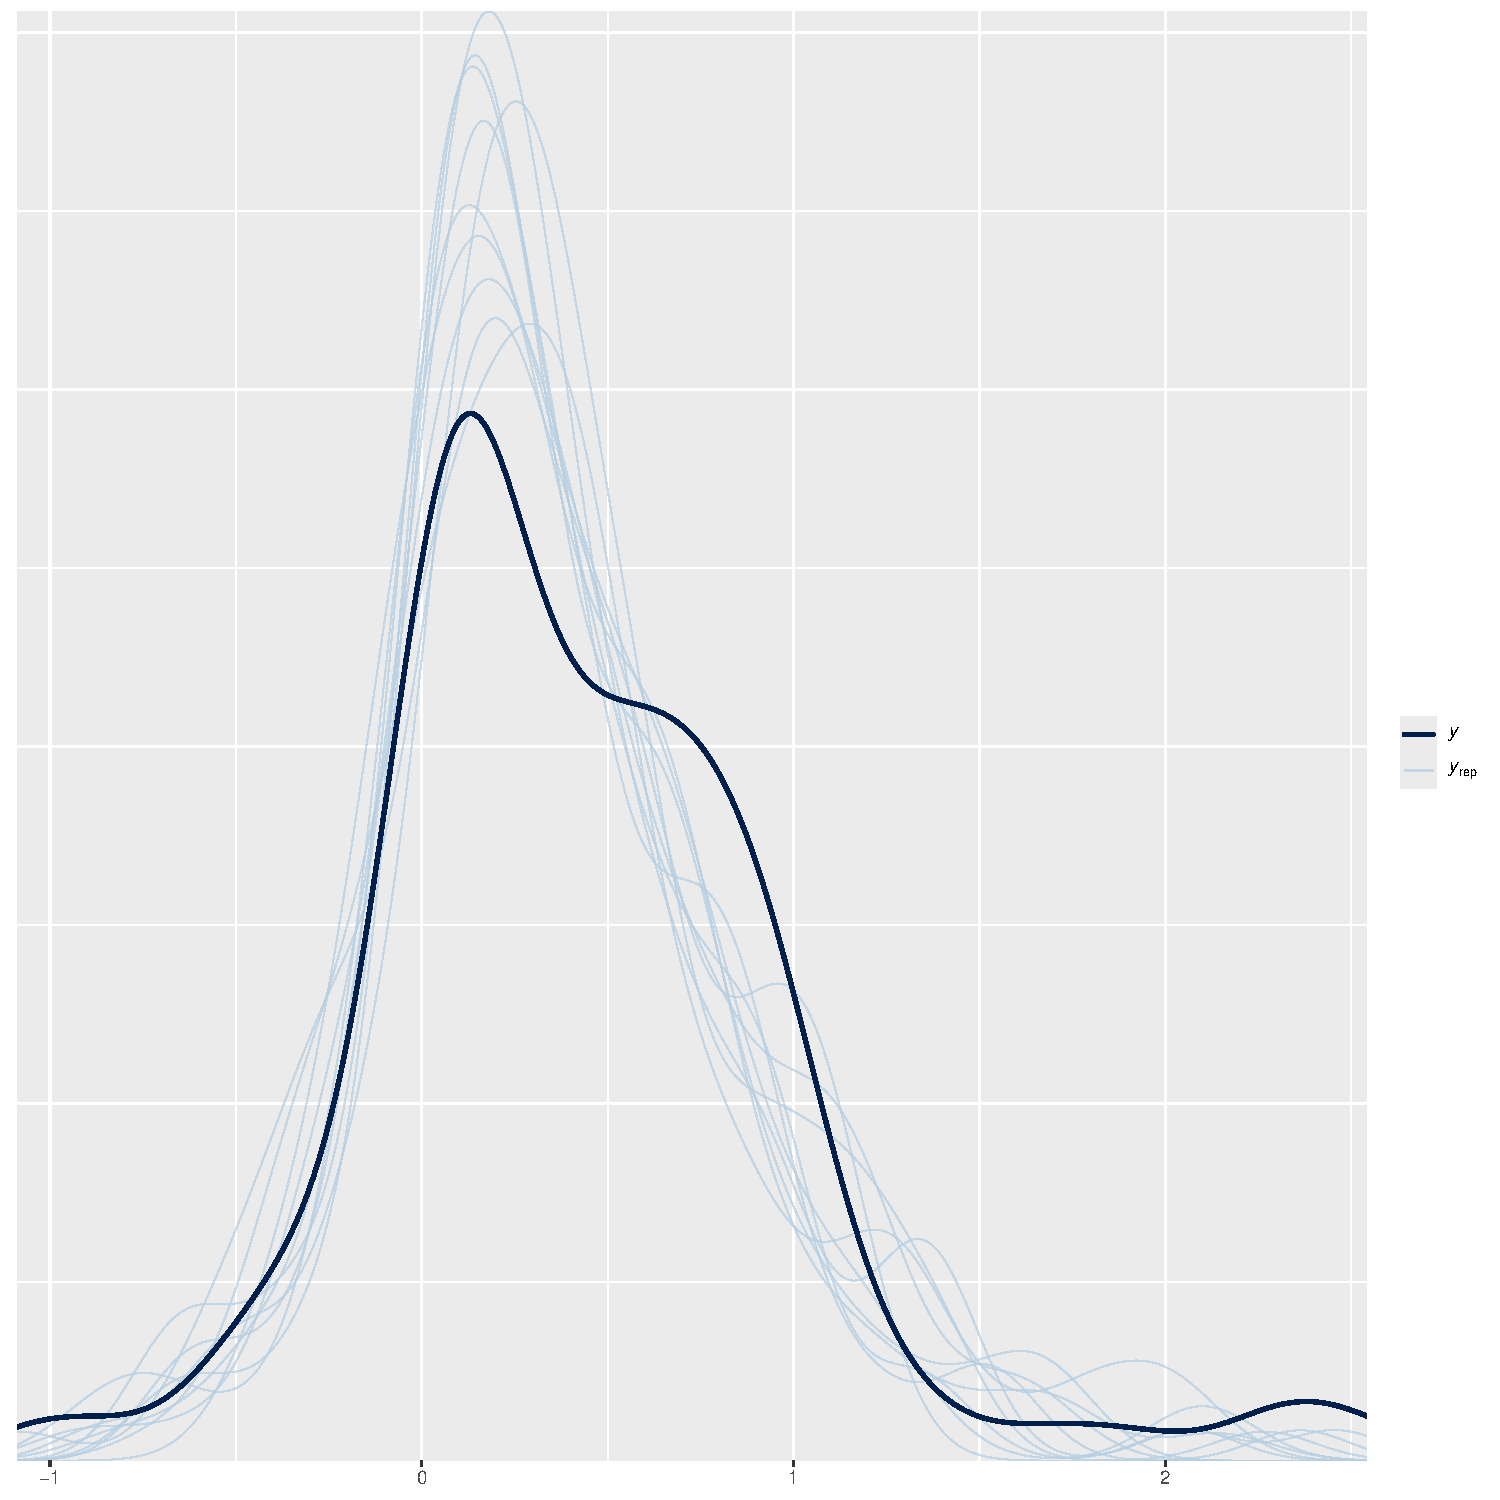
\includegraphics[width=1\textwidth,height=\textheight]{diagnostic_plots_files/figure-pdf/unnamed-chunk-12-1.pdf}

}

\end{figure}

\hypertarget{matching-model}{%
\chapter{Matching Model}\label{matching-model}}

\hypertarget{hatr-4}{%
\section{\texorpdfstring{\(\hat{R}\)}{\textbackslash hat\{R\}}}\label{hatr-4}}

\begin{figure}

{\centering 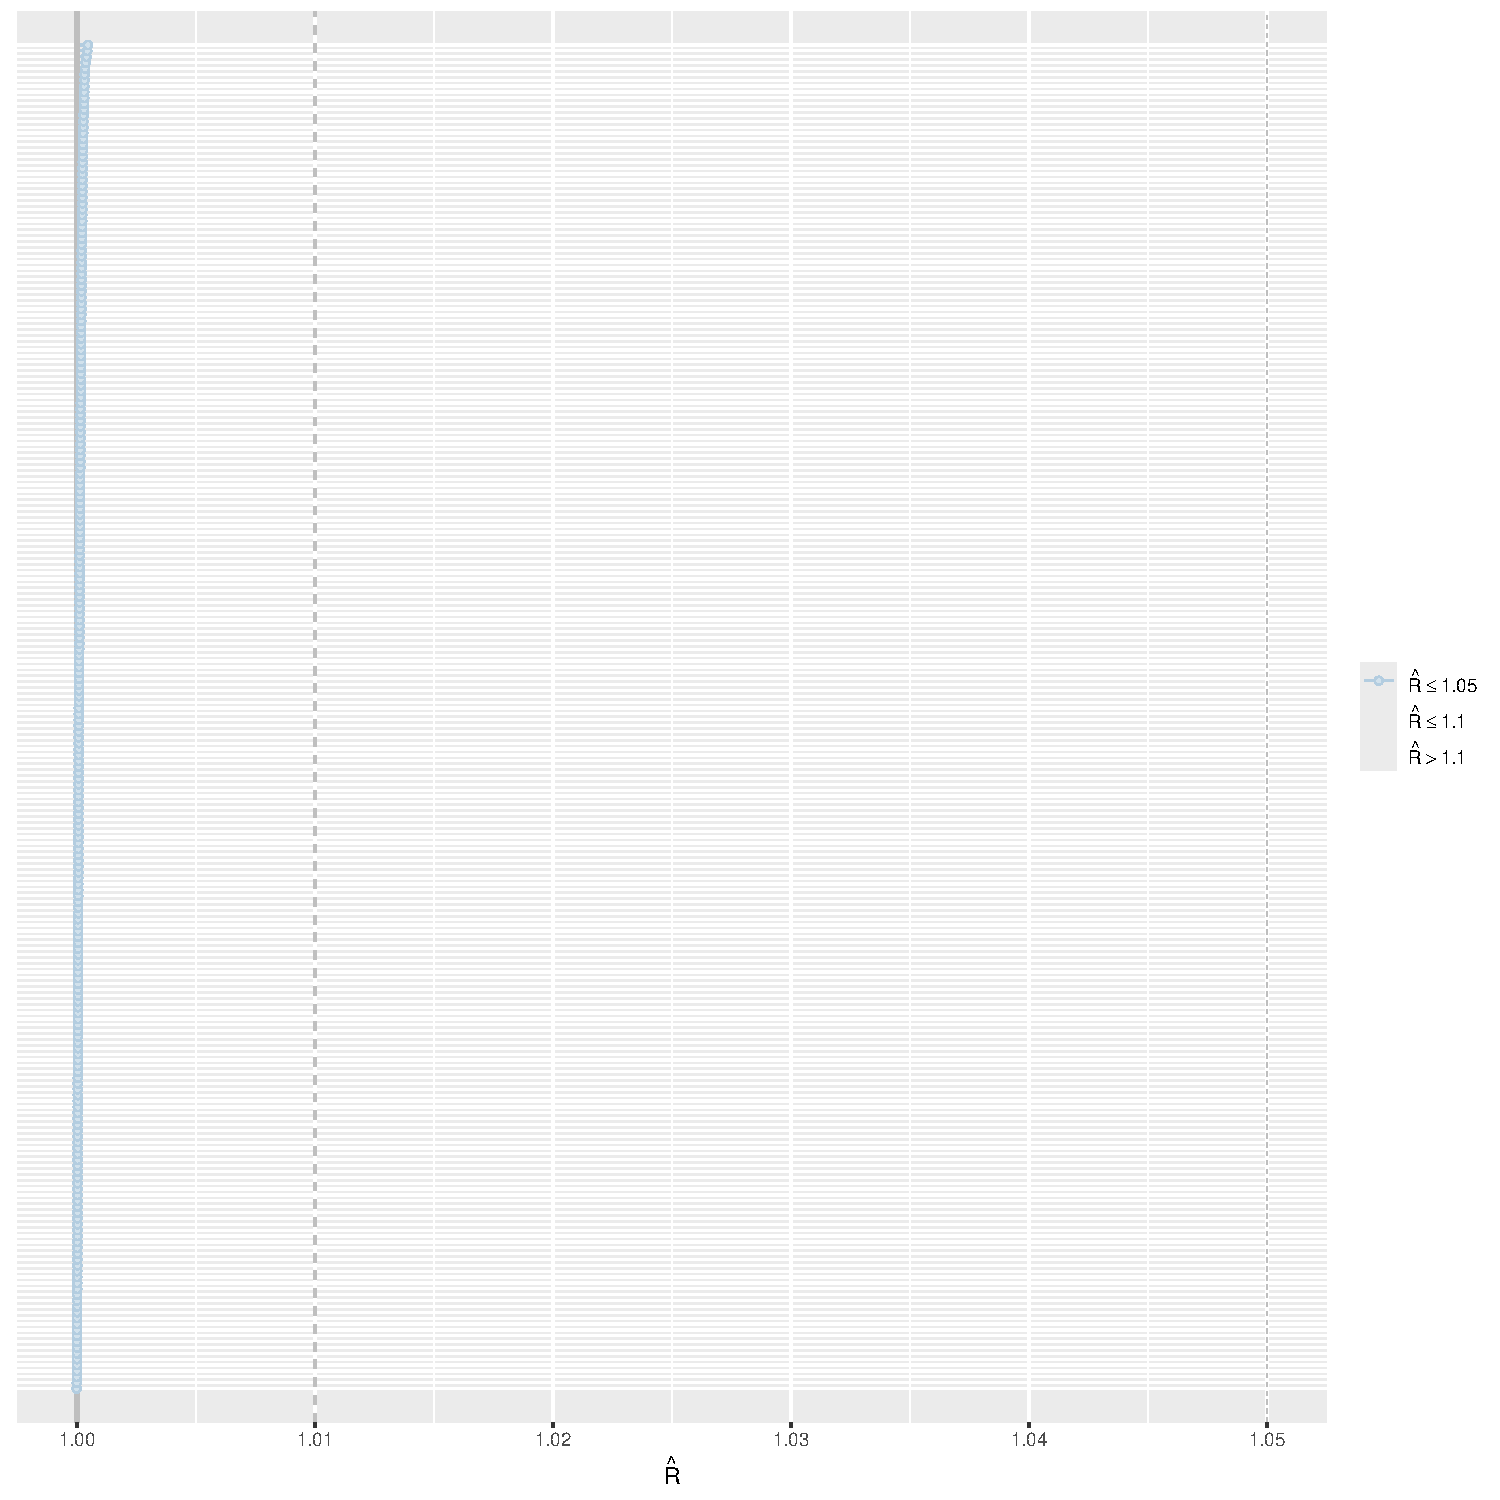
\includegraphics[width=1\textwidth,height=\textheight]{diagnostic_plots_files/figure-pdf/unnamed-chunk-13-1.pdf}

}

\end{figure}

\hypertarget{trace-plots-4}{%
\section{Trace plots}\label{trace-plots-4}}

\begin{figure}

{\centering 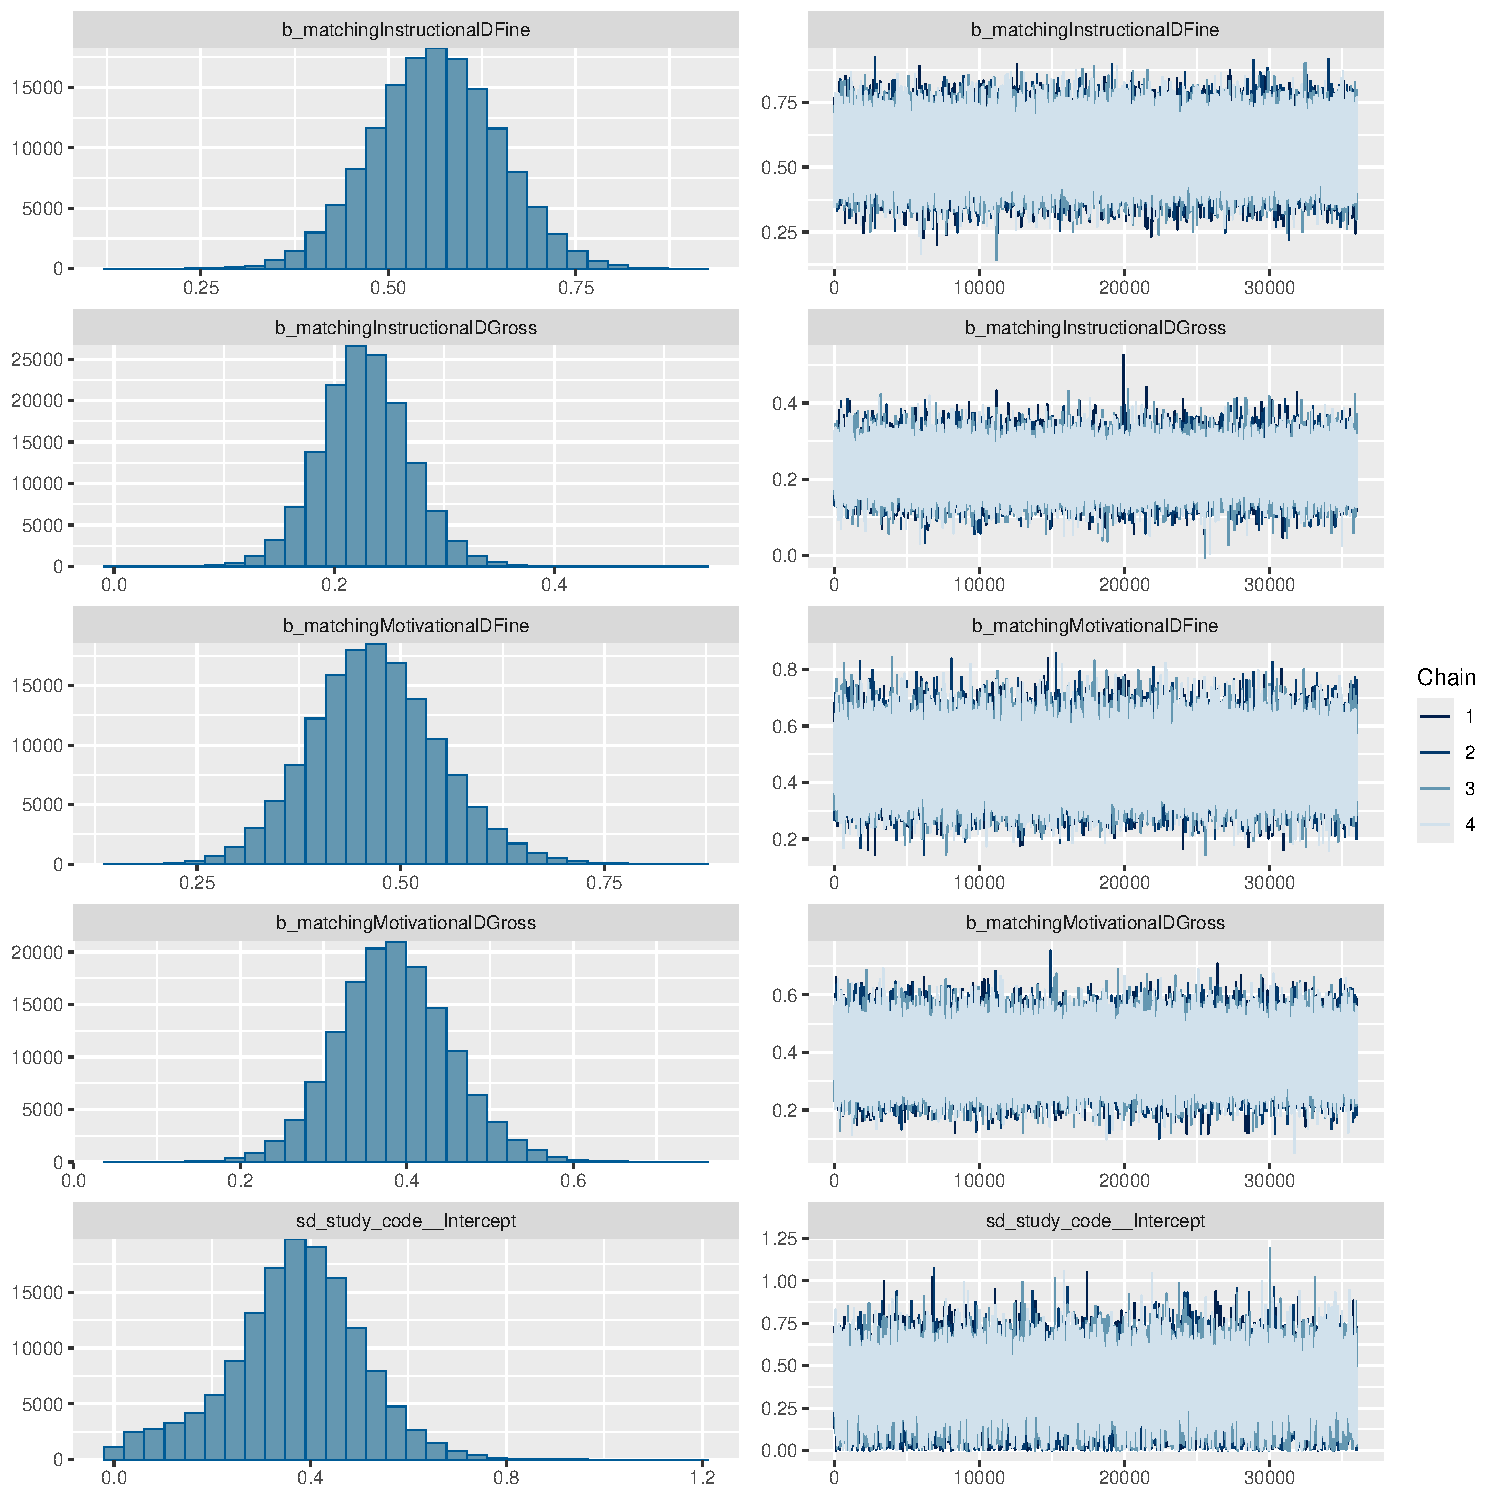
\includegraphics[width=1\textwidth,height=\textheight]{diagnostic_plots_files/figure-pdf/unnamed-chunk-14-1.pdf}

}

\end{figure}

\begin{figure}

{\centering 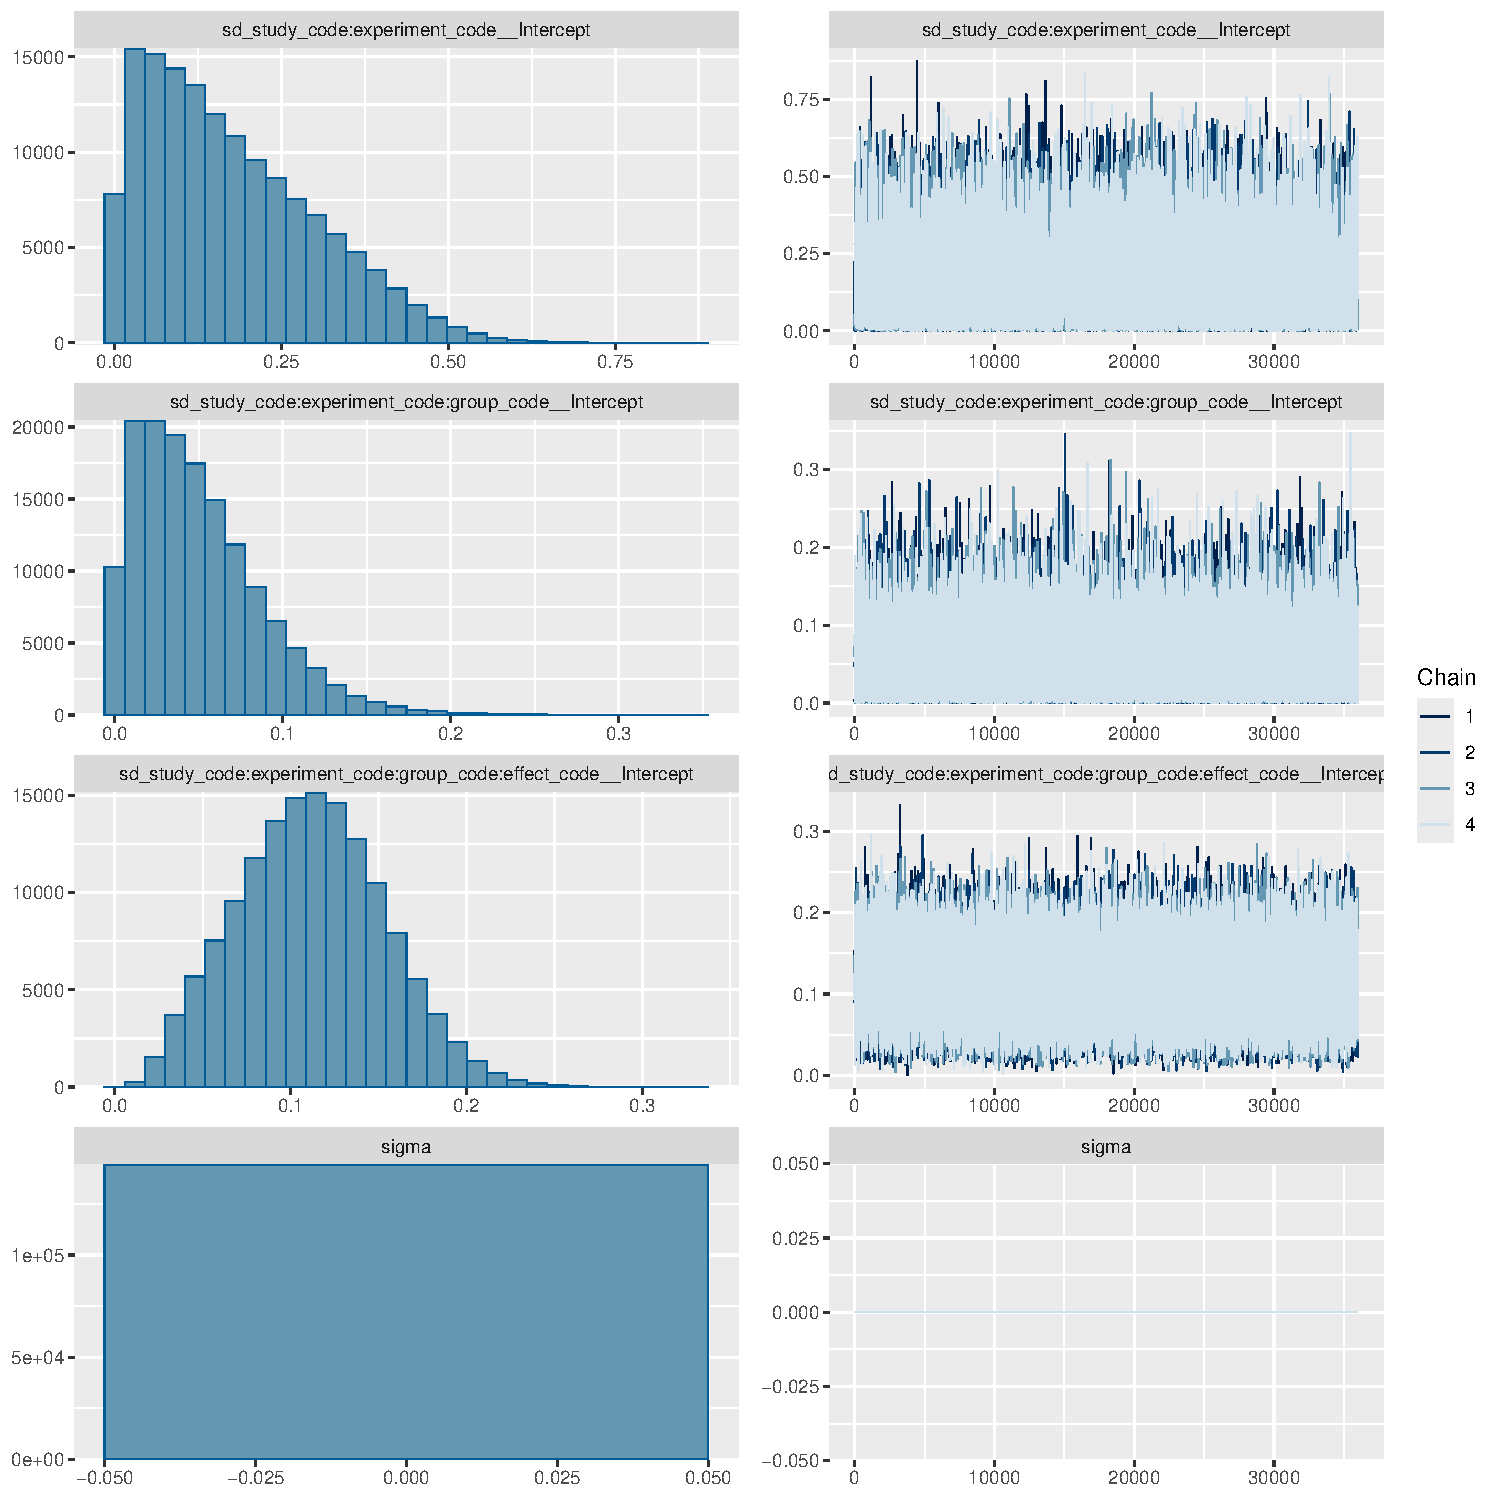
\includegraphics[width=1\textwidth,height=\textheight]{diagnostic_plots_files/figure-pdf/unnamed-chunk-14-2.pdf}

}

\end{figure}

\begin{verbatim}
[[1]]

[[2]]
\end{verbatim}

\hypertarget{posterior-predictive-check-4}{%
\section{Posterior predictive
check}\label{posterior-predictive-check-4}}

\begin{figure}

{\centering 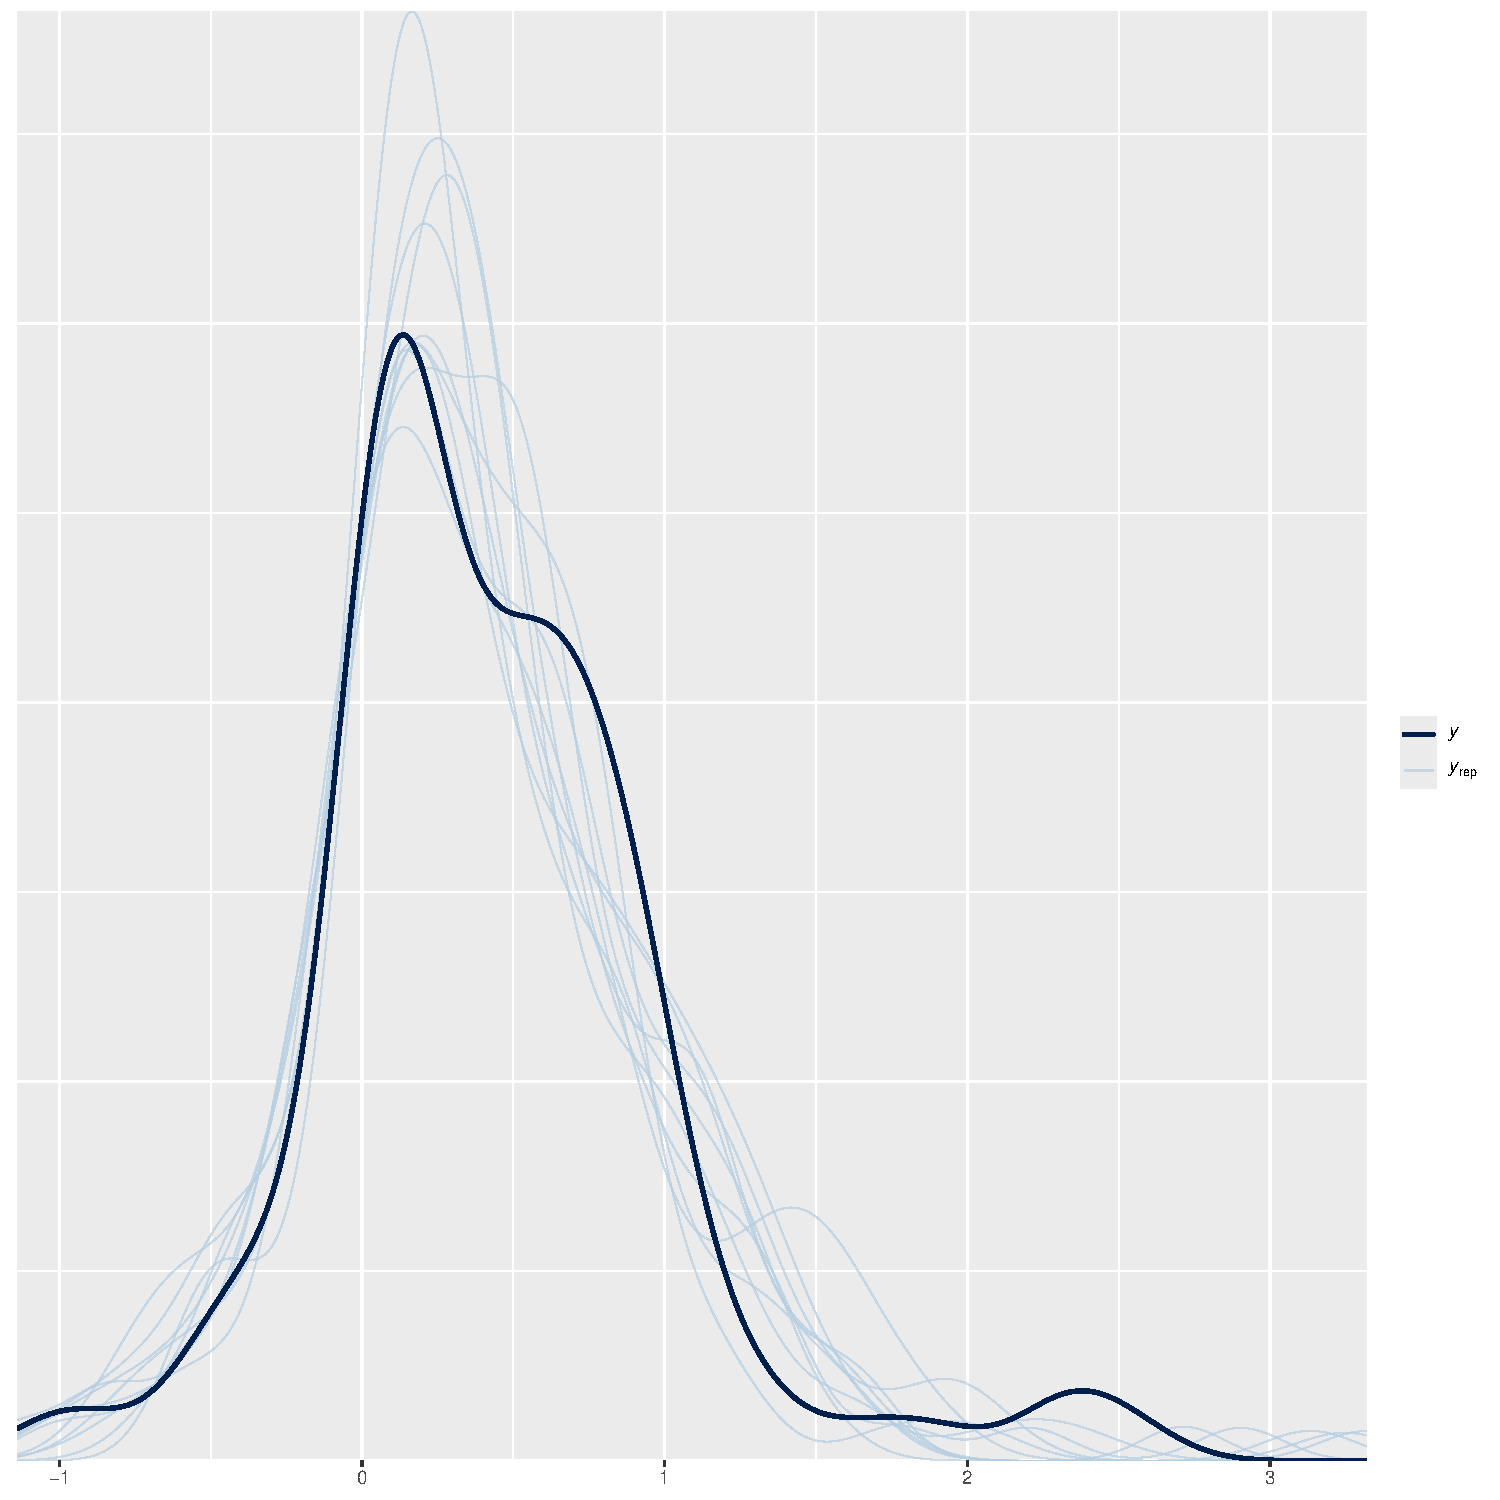
\includegraphics[width=1\textwidth,height=\textheight]{diagnostic_plots_files/figure-pdf/unnamed-chunk-15-1.pdf}

}

\end{figure}

\hypertarget{task_novelty-model}{%
\chapter{task\_novelty Model}\label{task_novelty-model}}

\hypertarget{hatr-5}{%
\section{\texorpdfstring{\(\hat{R}\)}{\textbackslash hat\{R\}}}\label{hatr-5}}

\begin{figure}

{\centering 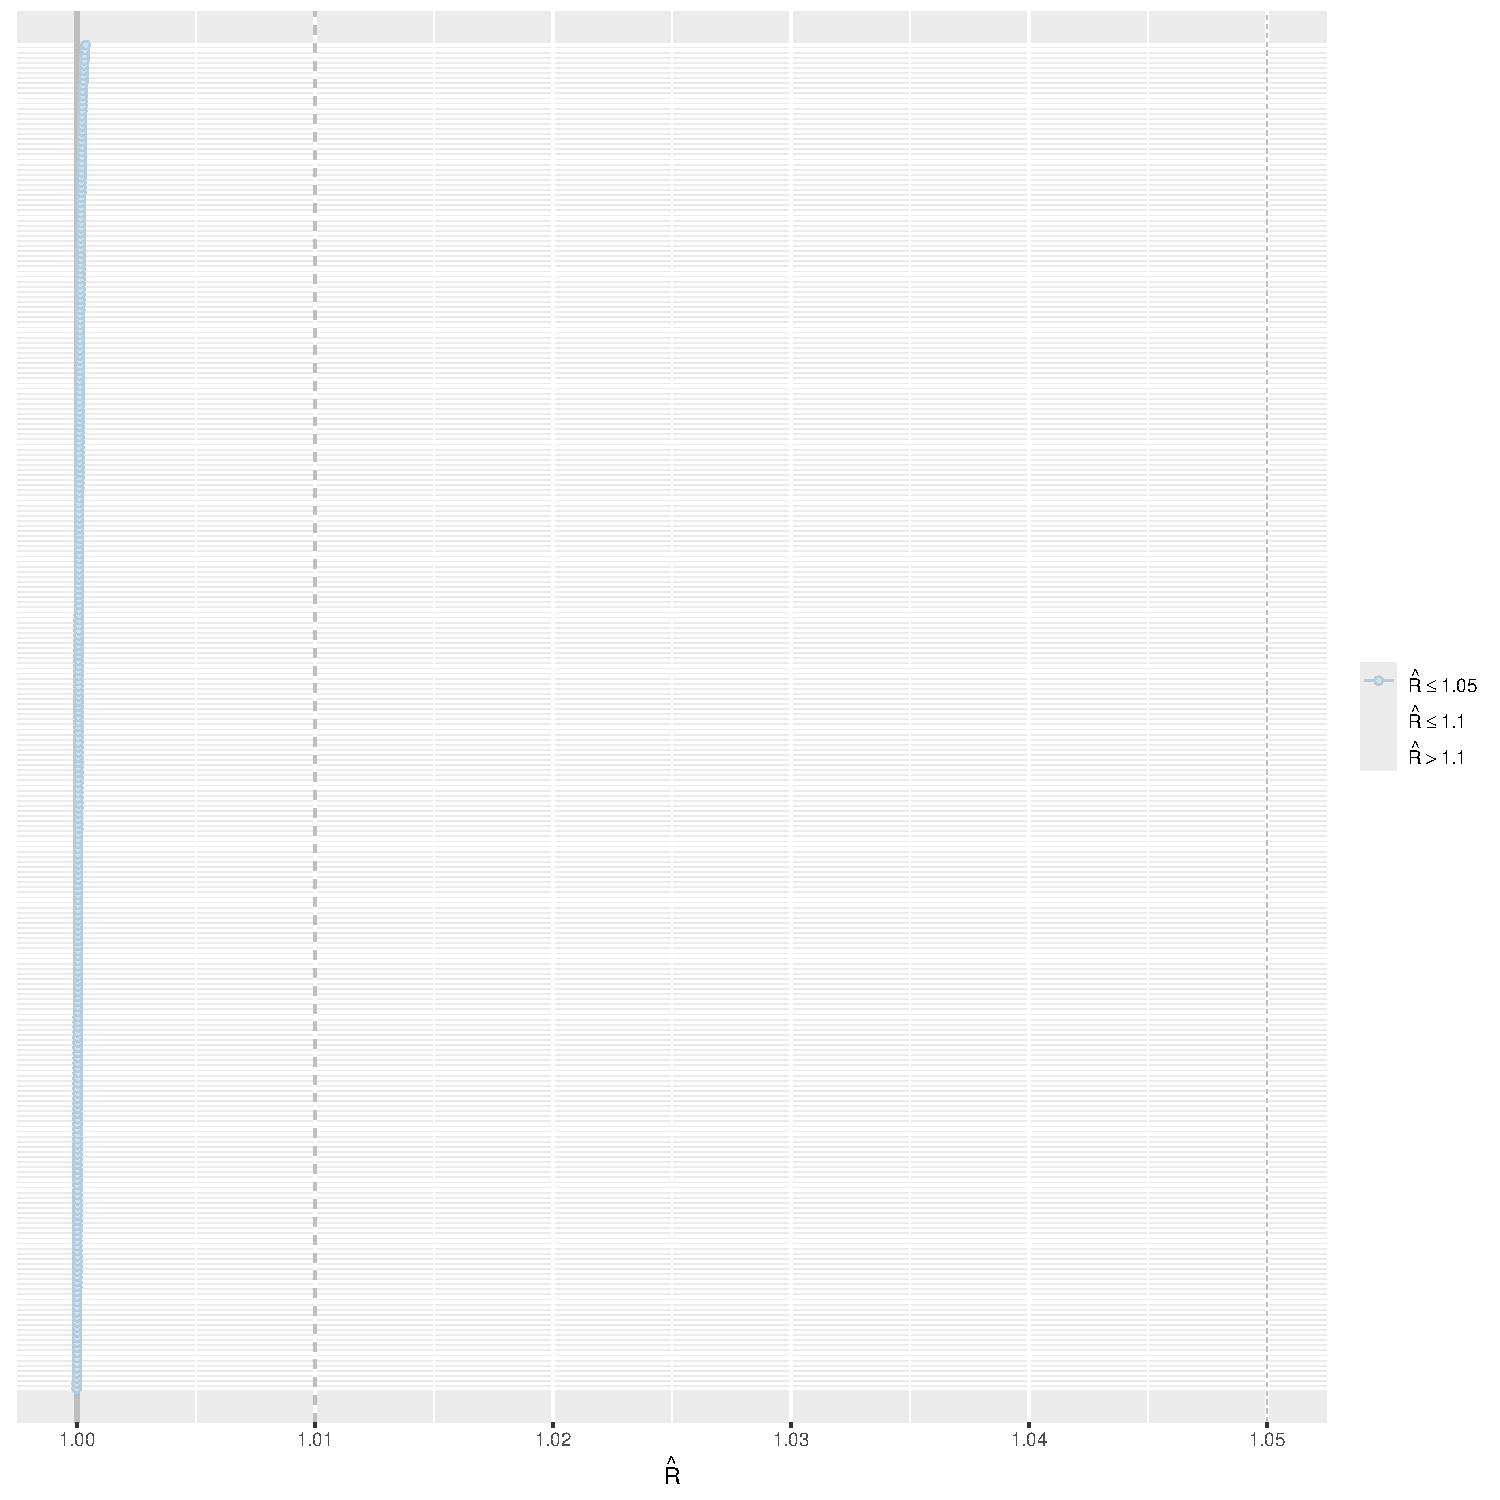
\includegraphics[width=1\textwidth,height=\textheight]{diagnostic_plots_files/figure-pdf/unnamed-chunk-16-1.pdf}

}

\end{figure}

\hypertarget{trace-plots-5}{%
\section{Trace plots}\label{trace-plots-5}}

\begin{figure}

{\centering 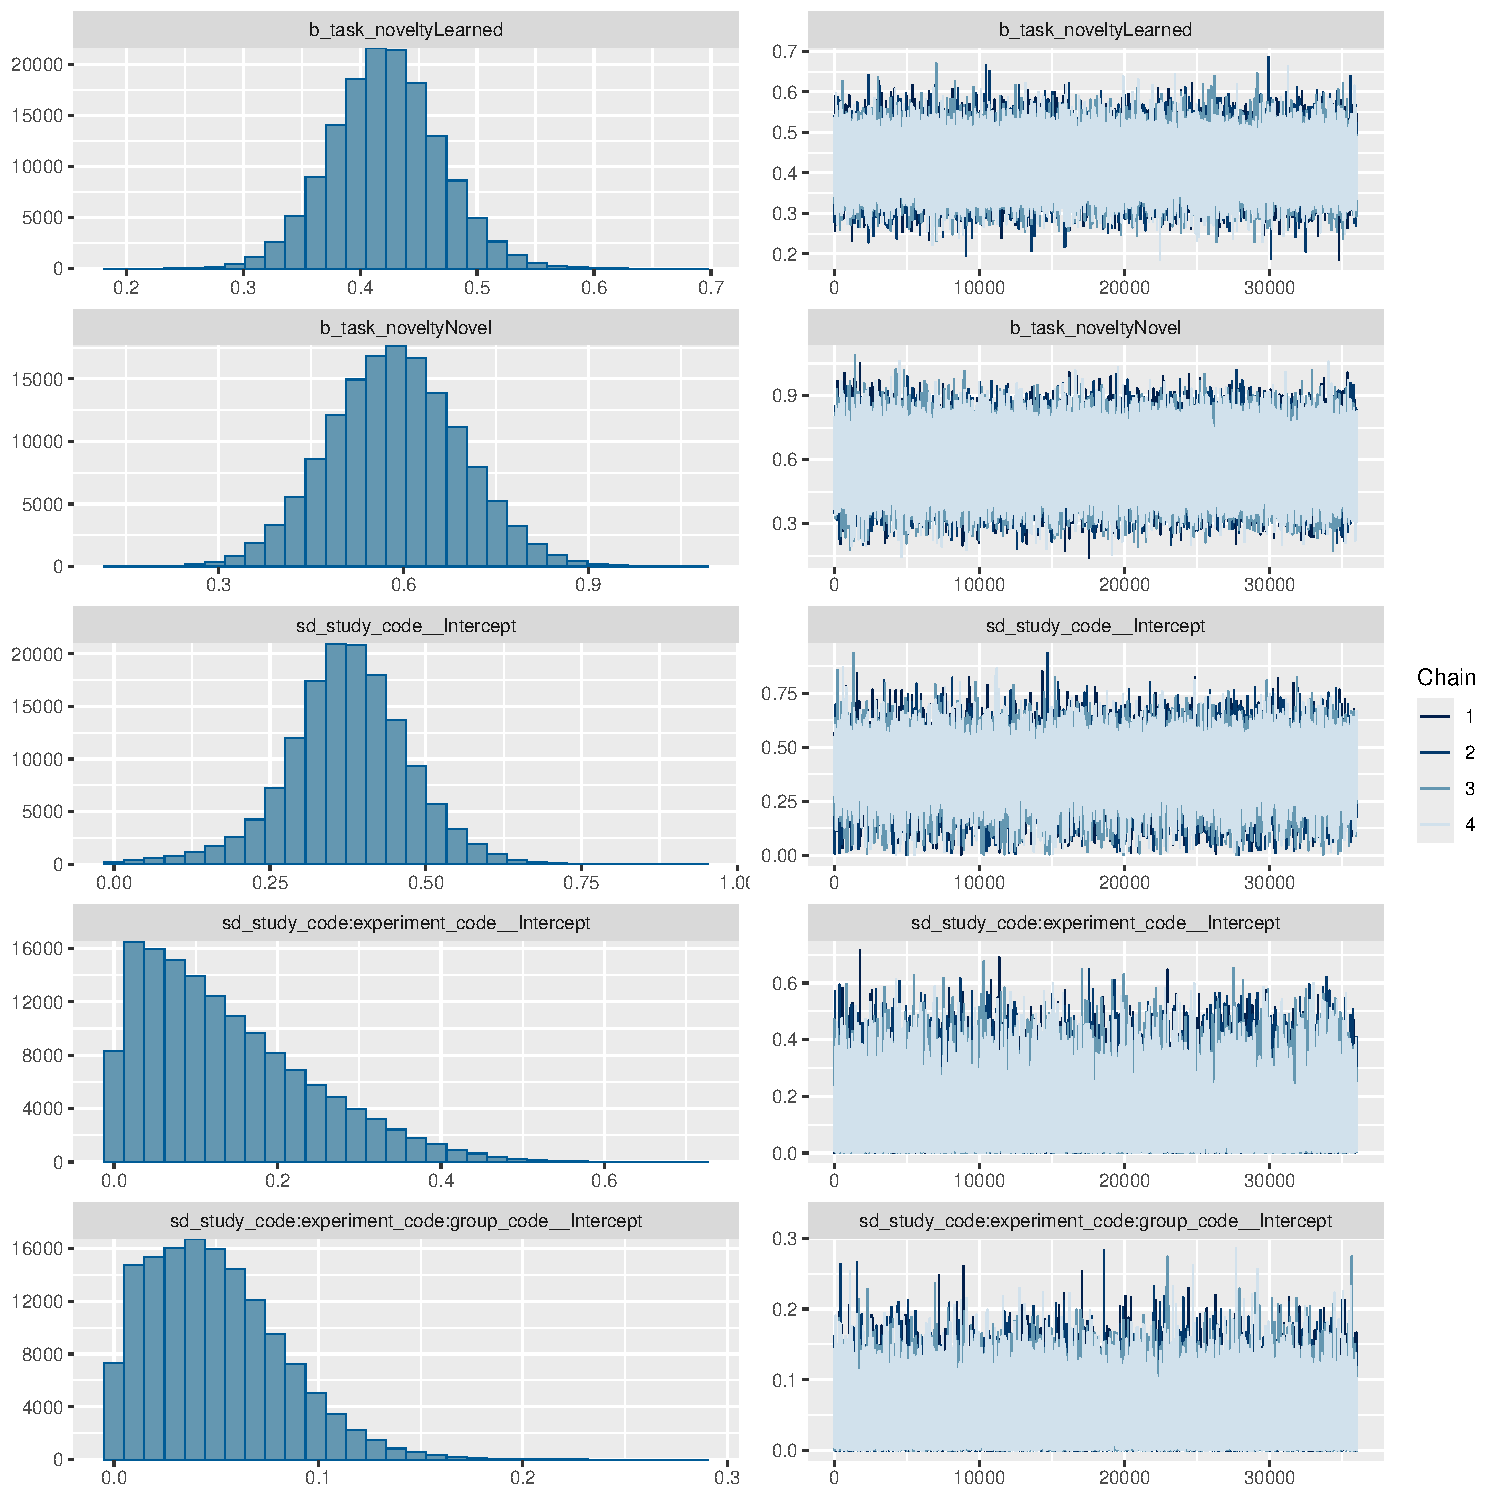
\includegraphics[width=1\textwidth,height=\textheight]{diagnostic_plots_files/figure-pdf/unnamed-chunk-17-1.pdf}

}

\end{figure}

\begin{figure}

{\centering 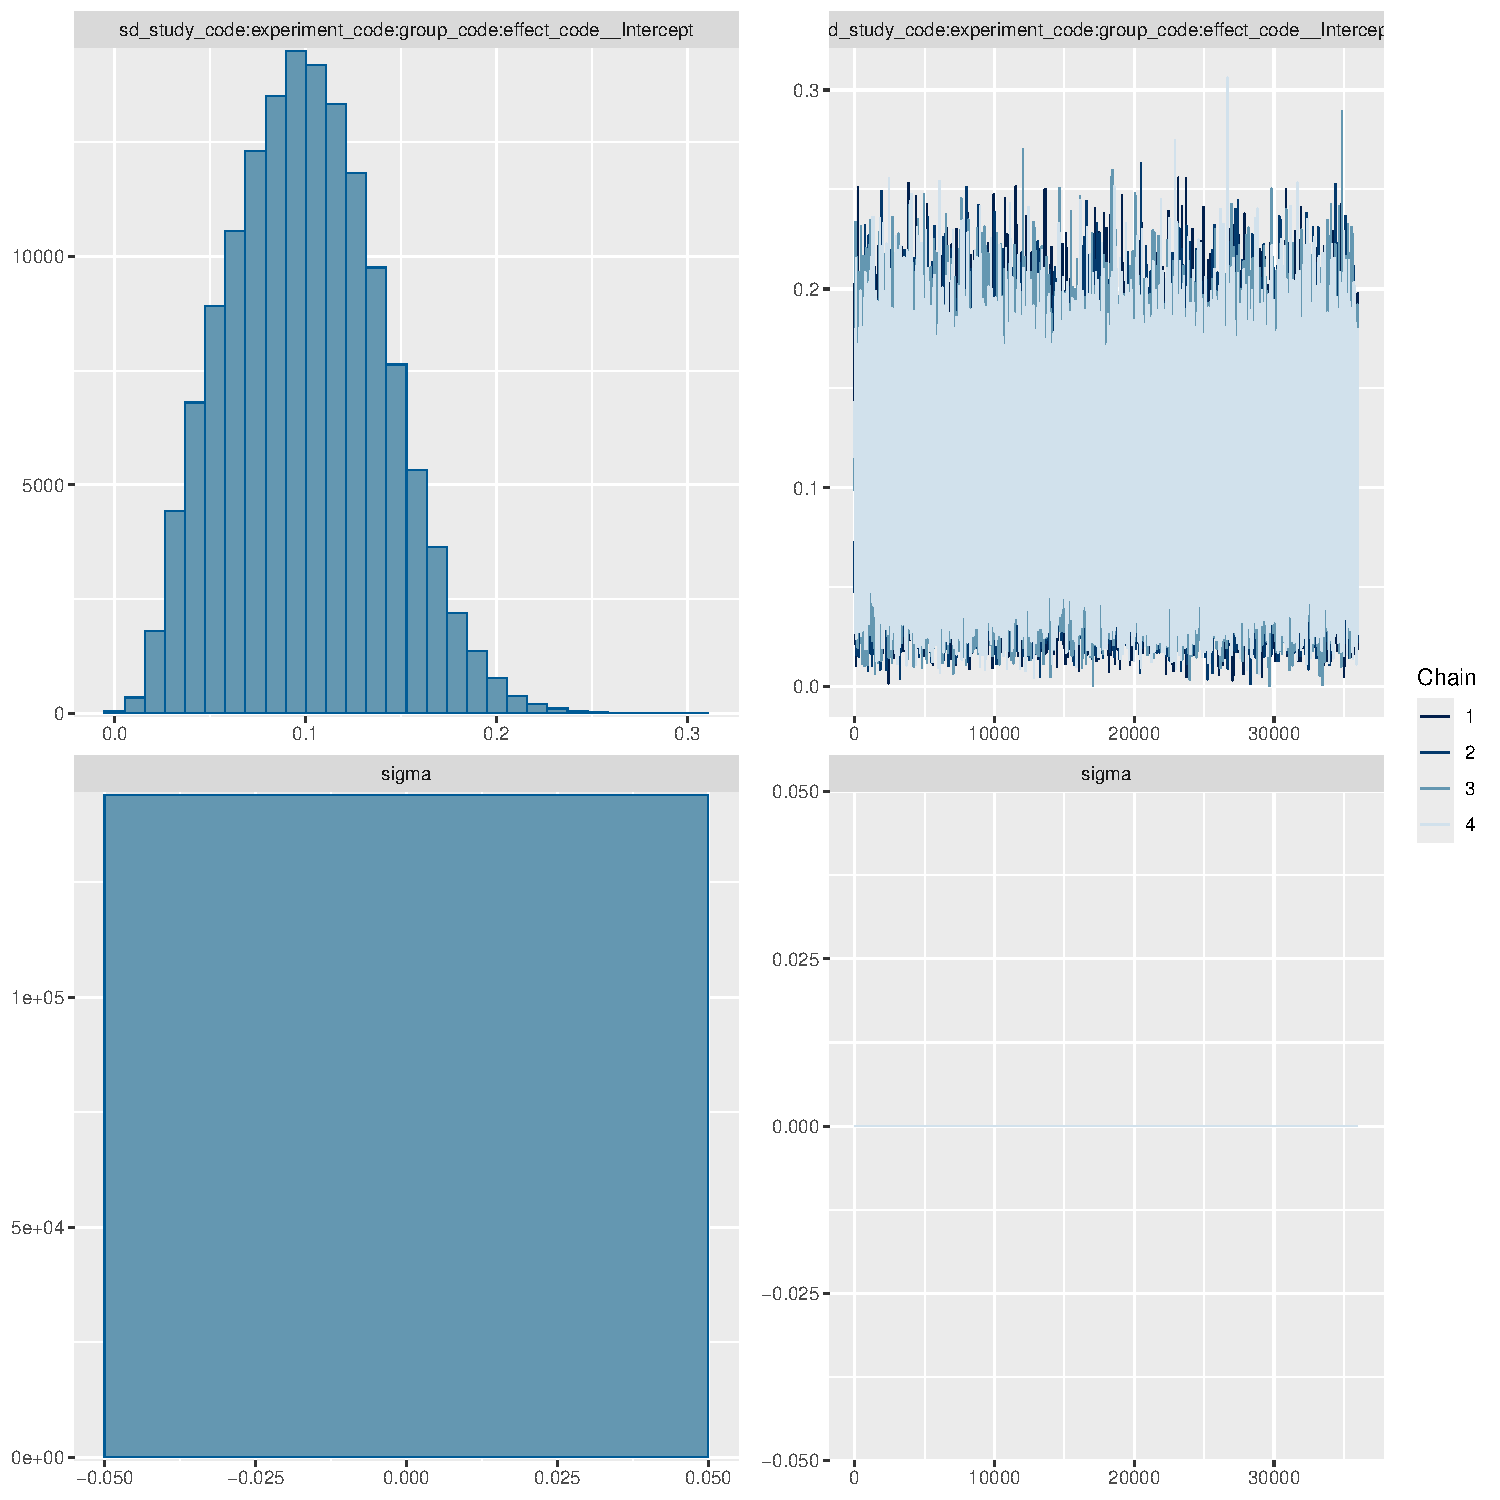
\includegraphics[width=1\textwidth,height=\textheight]{diagnostic_plots_files/figure-pdf/unnamed-chunk-17-2.pdf}

}

\end{figure}

\begin{verbatim}
[[1]]

[[2]]
\end{verbatim}

\hypertarget{posterior-predictive-check-5}{%
\section{Posterior predictive
check}\label{posterior-predictive-check-5}}

\begin{figure}

{\centering 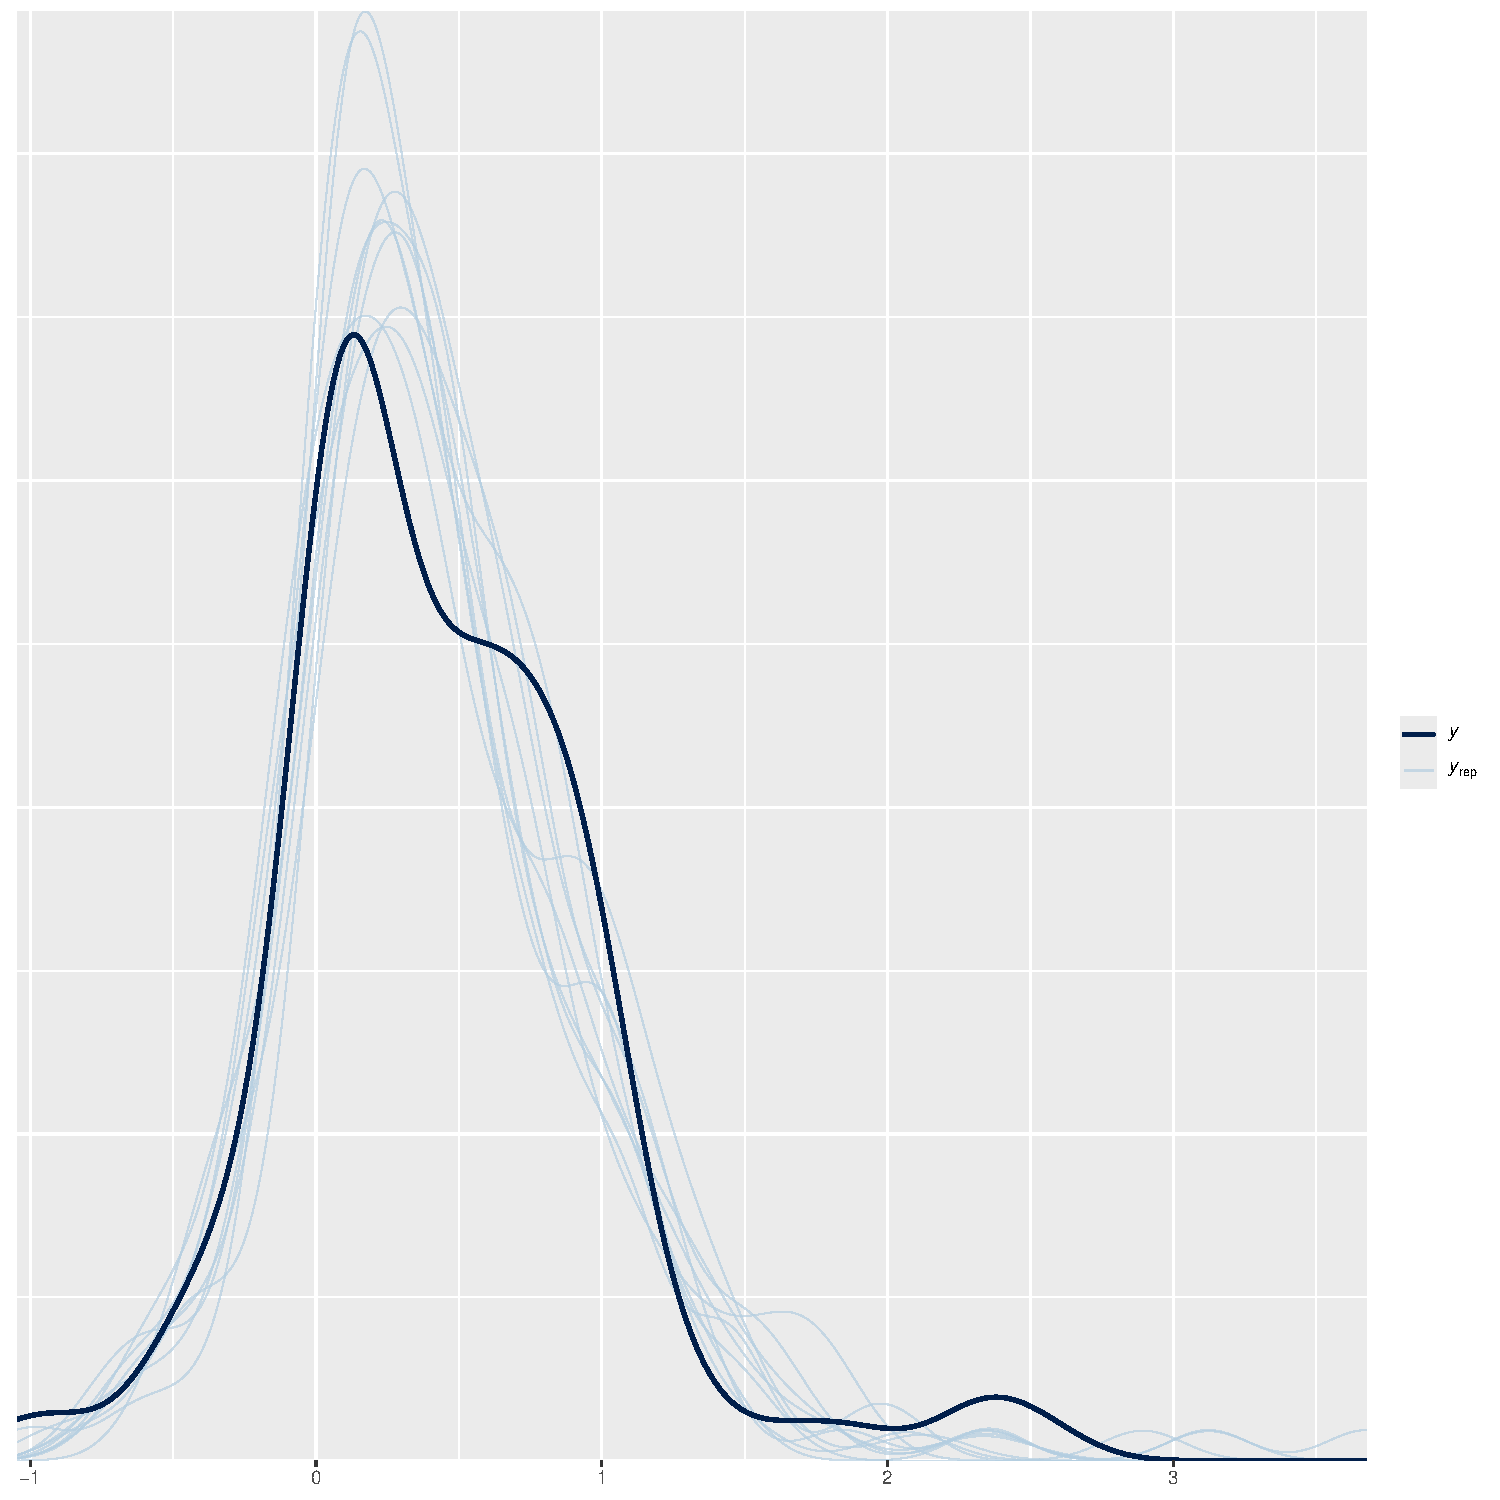
\includegraphics[width=1\textwidth,height=\textheight]{diagnostic_plots_files/figure-pdf/unnamed-chunk-18-1.pdf}

}

\end{figure}

\hypertarget{cue-selection-model}{%
\chapter{Cue Selection Model}\label{cue-selection-model}}

\hypertarget{hatr-6}{%
\section{\texorpdfstring{\(\hat{R}\)}{\textbackslash hat\{R\}}}\label{hatr-6}}

\begin{figure}

{\centering 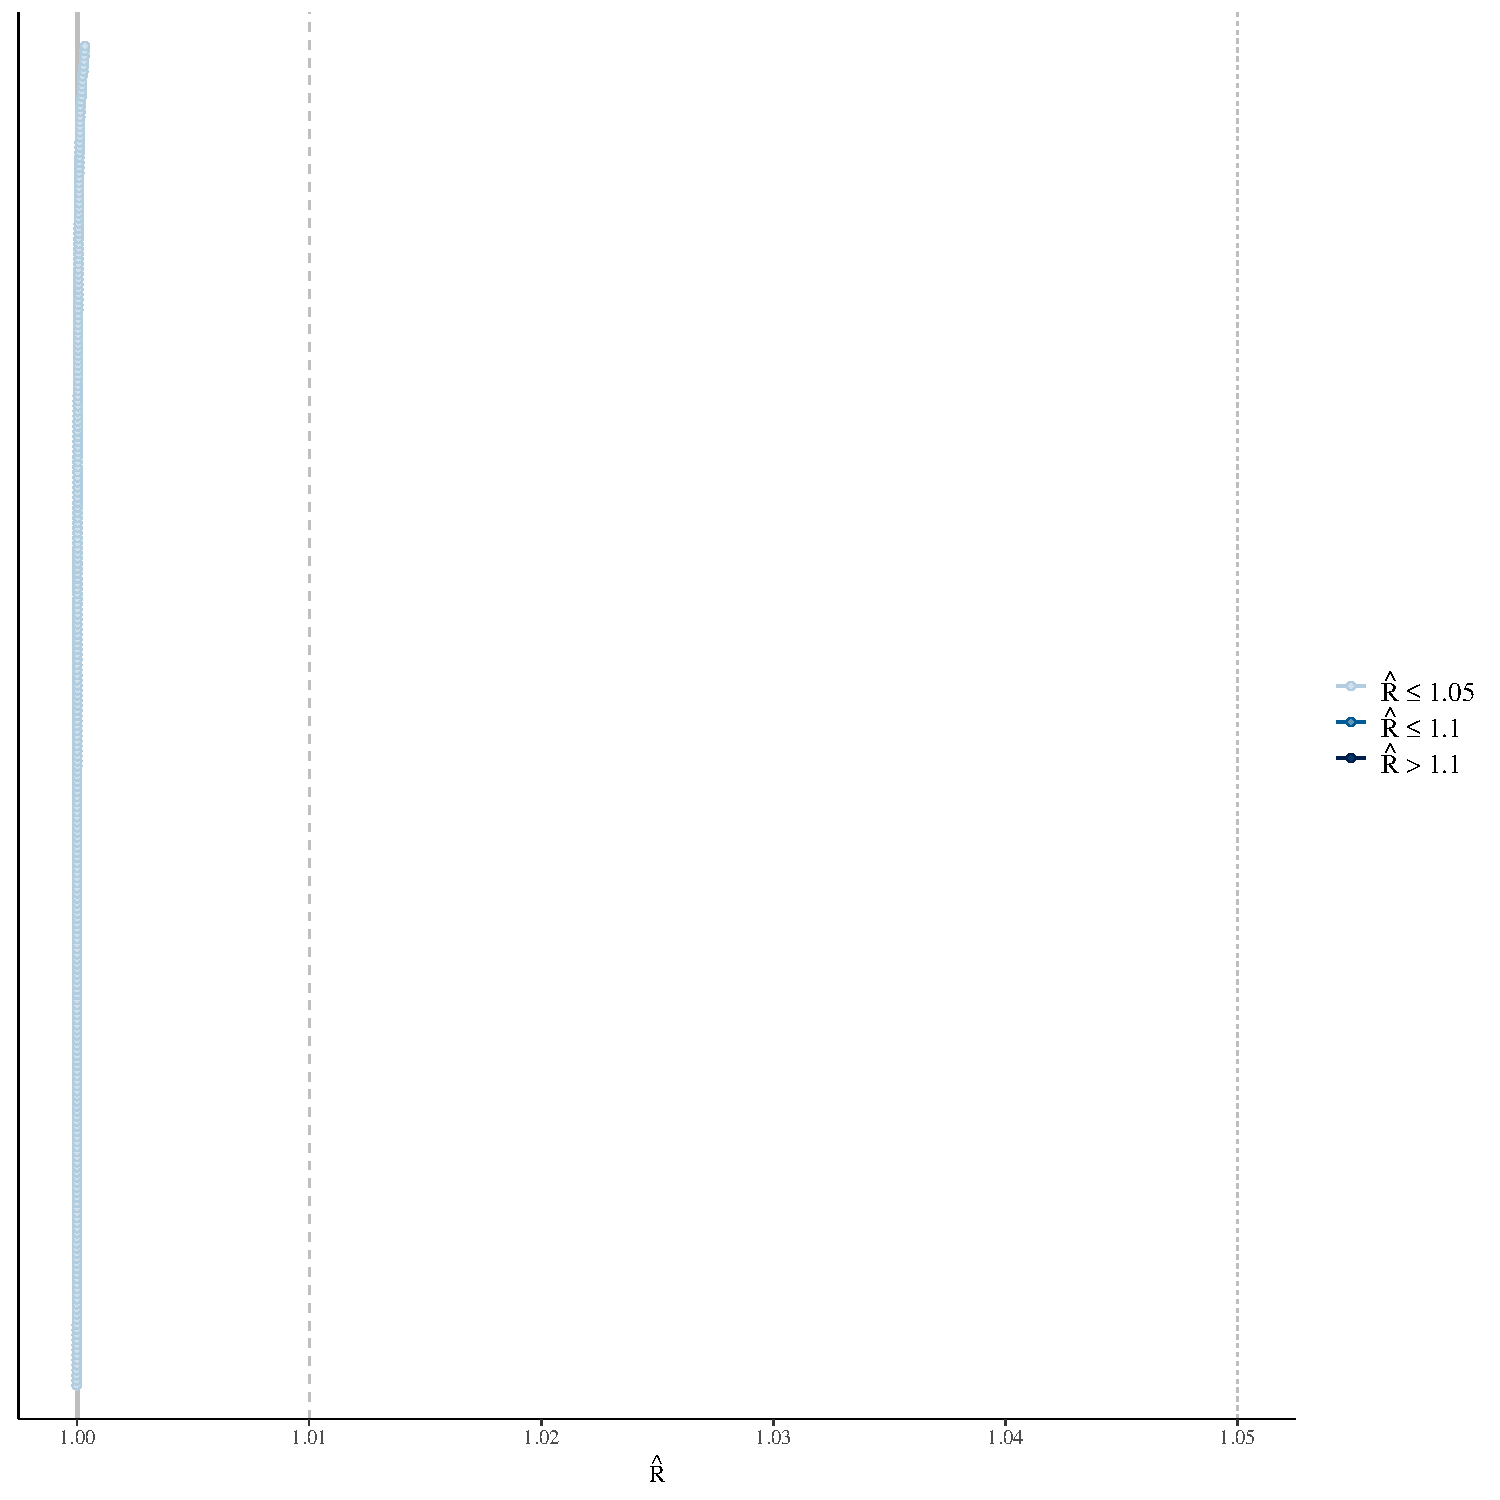
\includegraphics[width=1\textwidth,height=\textheight]{diagnostic_plots_files/figure-pdf/unnamed-chunk-19-1.pdf}

}

\end{figure}

\hypertarget{trace-plots-6}{%
\section{Trace plots}\label{trace-plots-6}}

\begin{figure}

{\centering 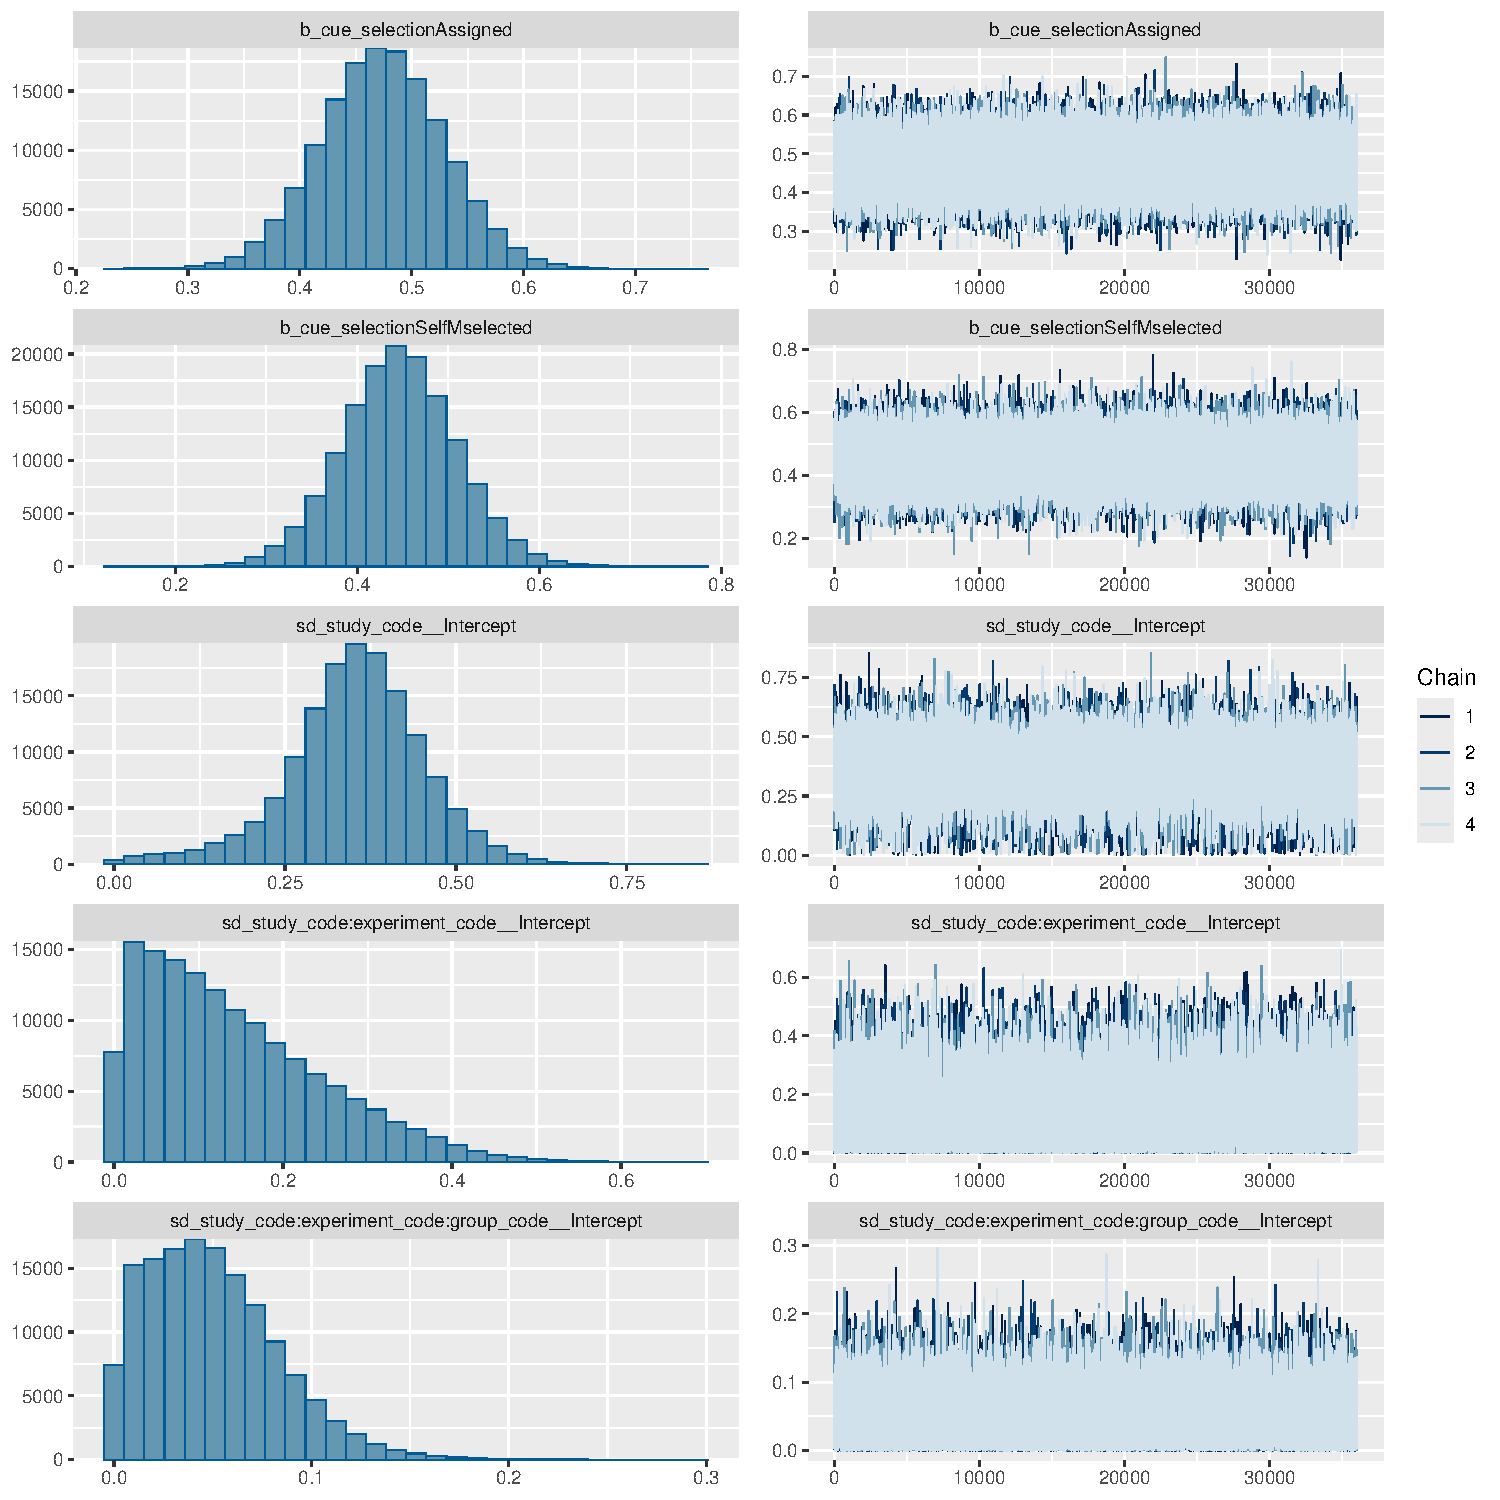
\includegraphics[width=1\textwidth,height=\textheight]{diagnostic_plots_files/figure-pdf/unnamed-chunk-20-1.pdf}

}

\end{figure}

\begin{figure}

{\centering 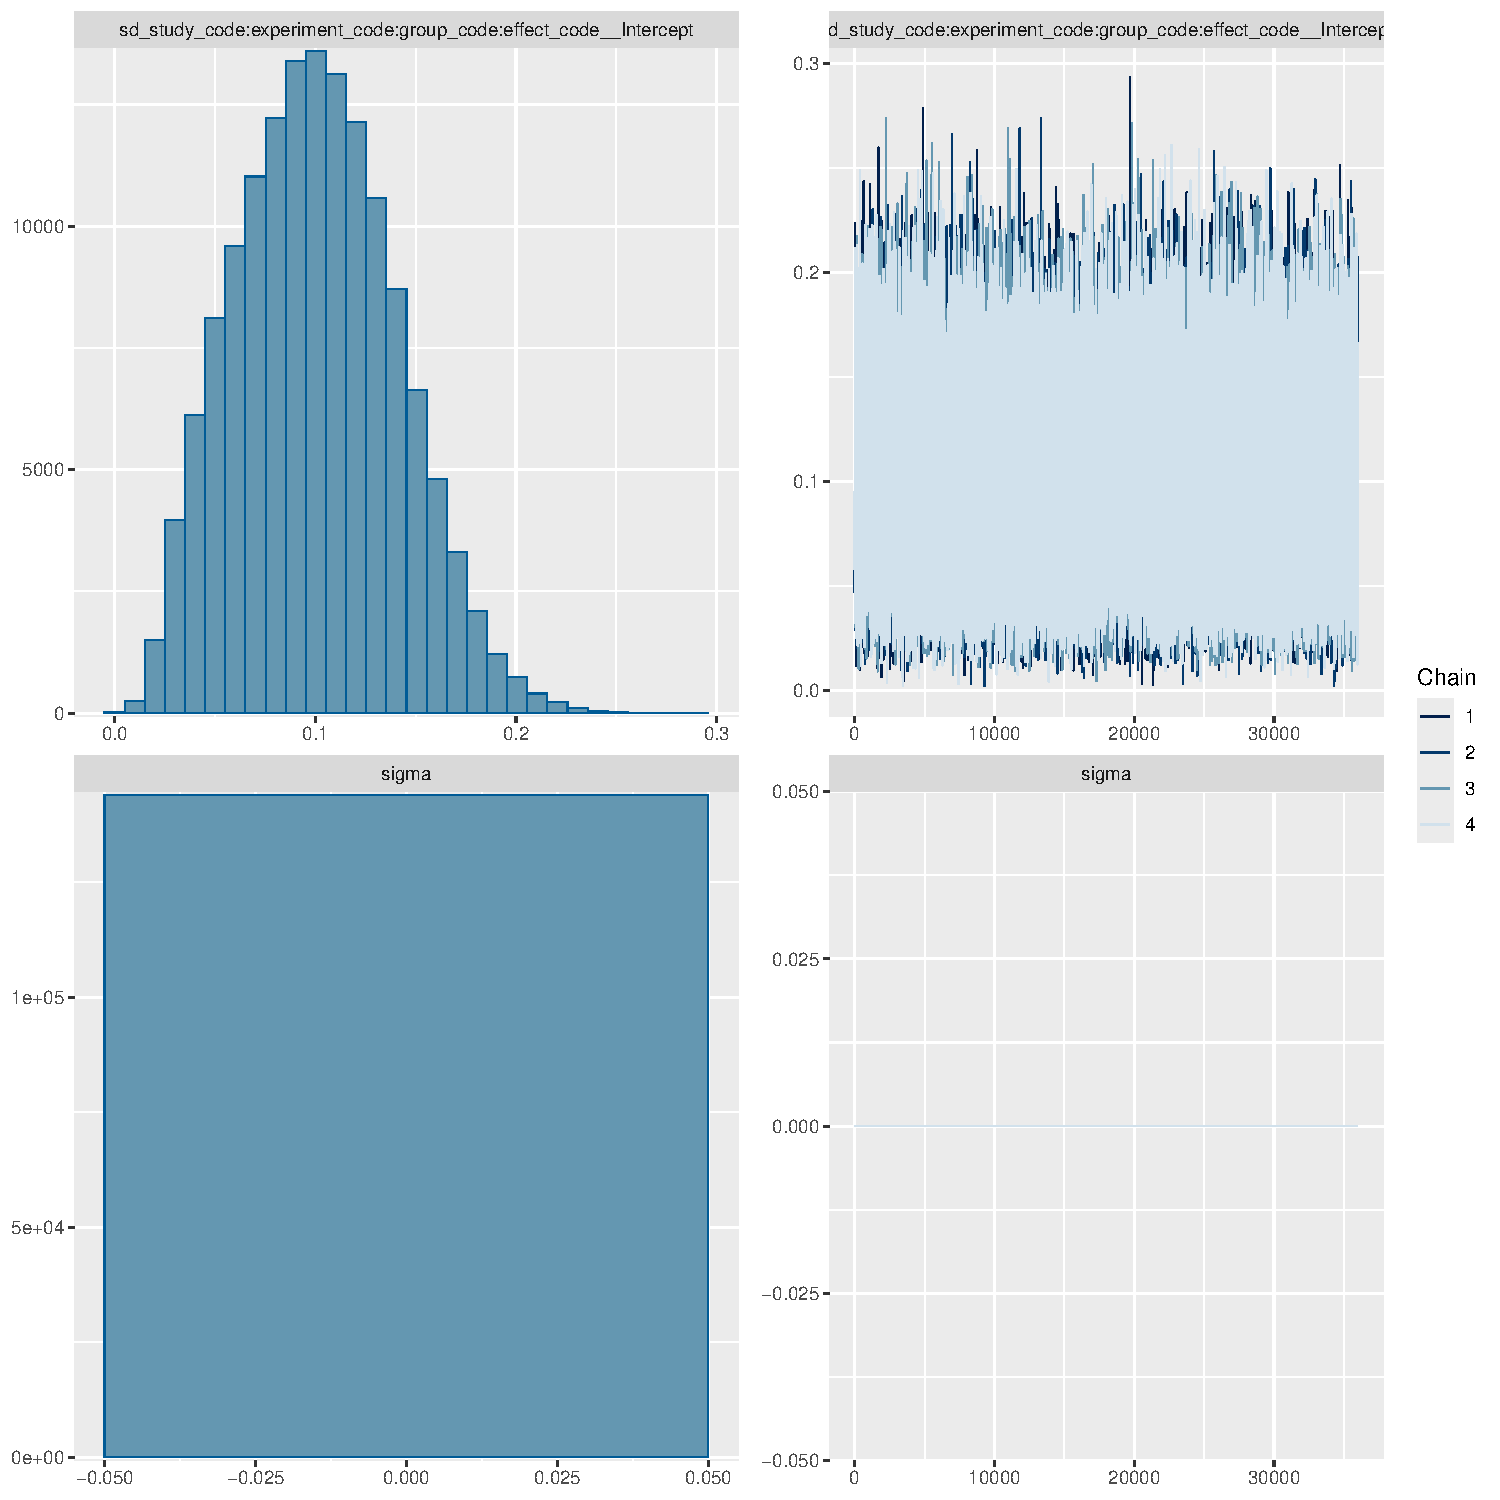
\includegraphics[width=1\textwidth,height=\textheight]{diagnostic_plots_files/figure-pdf/unnamed-chunk-20-2.pdf}

}

\end{figure}

\begin{verbatim}
[[1]]

[[2]]
\end{verbatim}

\hypertarget{posterior-predictive-check-6}{%
\section{Posterior predictive
check}\label{posterior-predictive-check-6}}

\begin{figure}

{\centering 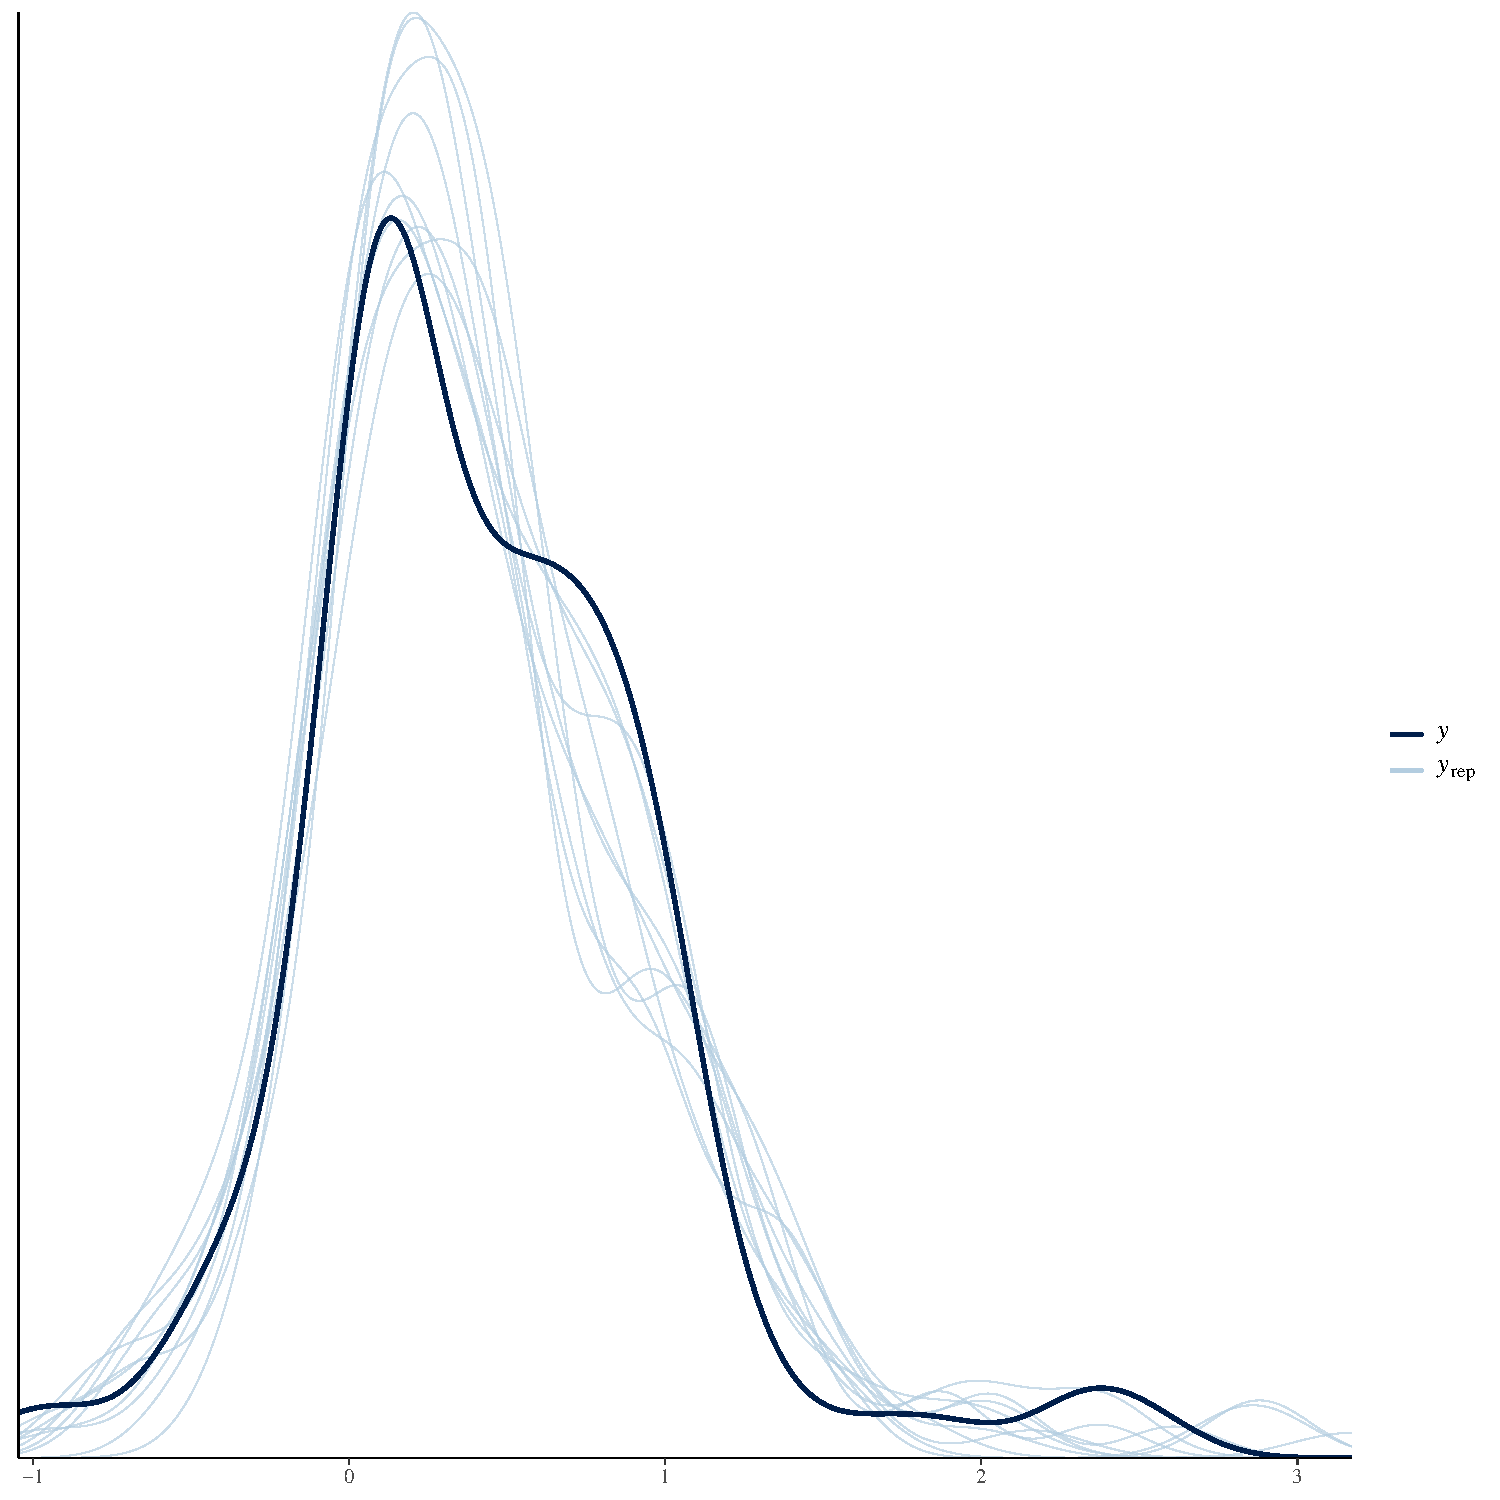
\includegraphics[width=1\textwidth,height=\textheight]{diagnostic_plots_files/figure-pdf/unnamed-chunk-21-1.pdf}

}

\end{figure}

\hypertarget{overtness-selection-model}{%
\chapter{Overtness Selection Model}\label{overtness-selection-model}}

\hypertarget{hatr-7}{%
\section{\texorpdfstring{\(\hat{R}\)}{\textbackslash hat\{R\}}}\label{hatr-7}}

\begin{figure}

{\centering 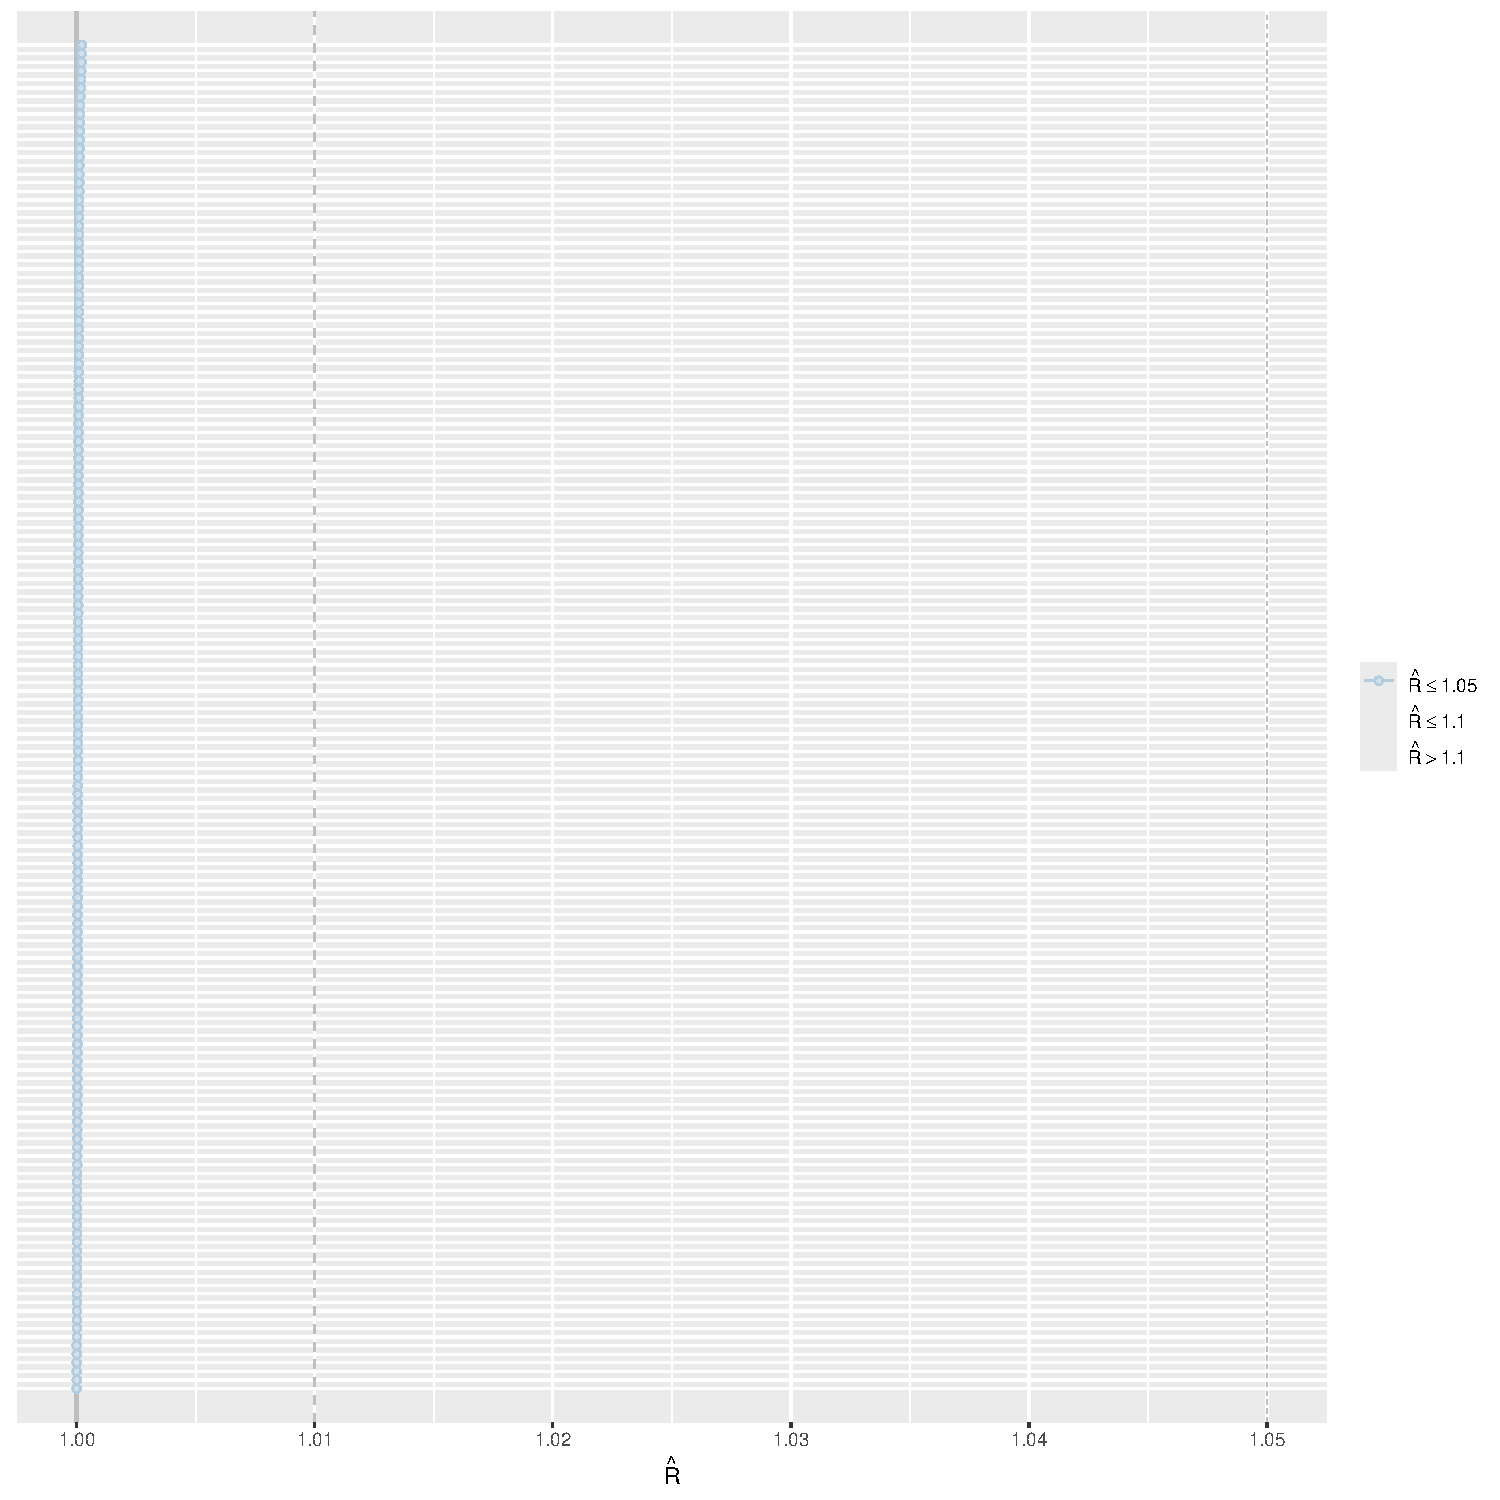
\includegraphics[width=1\textwidth,height=\textheight]{diagnostic_plots_files/figure-pdf/unnamed-chunk-22-1.pdf}

}

\end{figure}

\hypertarget{trace-plots-7}{%
\section{Trace plots}\label{trace-plots-7}}

\begin{figure}

{\centering 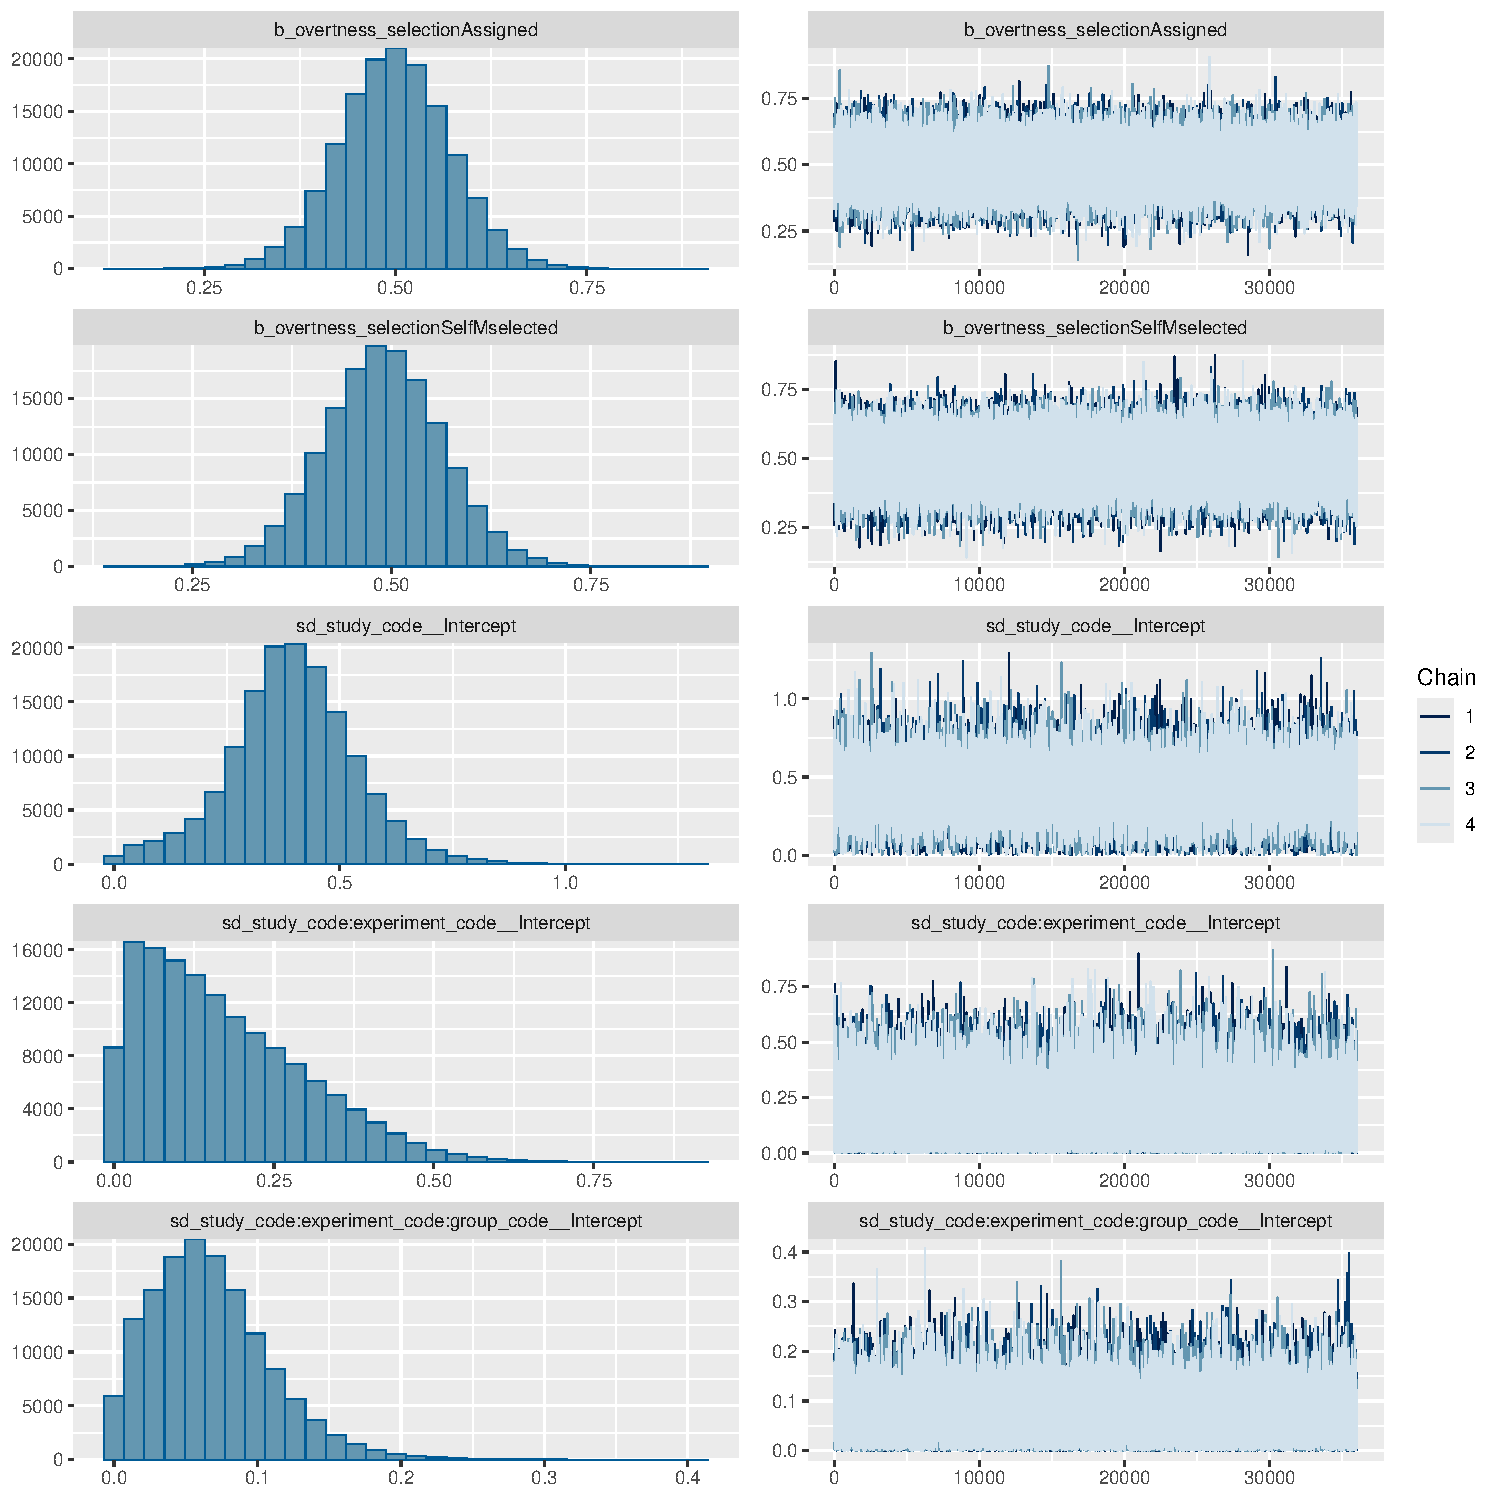
\includegraphics[width=1\textwidth,height=\textheight]{diagnostic_plots_files/figure-pdf/unnamed-chunk-23-1.pdf}

}

\end{figure}

\begin{figure}

{\centering 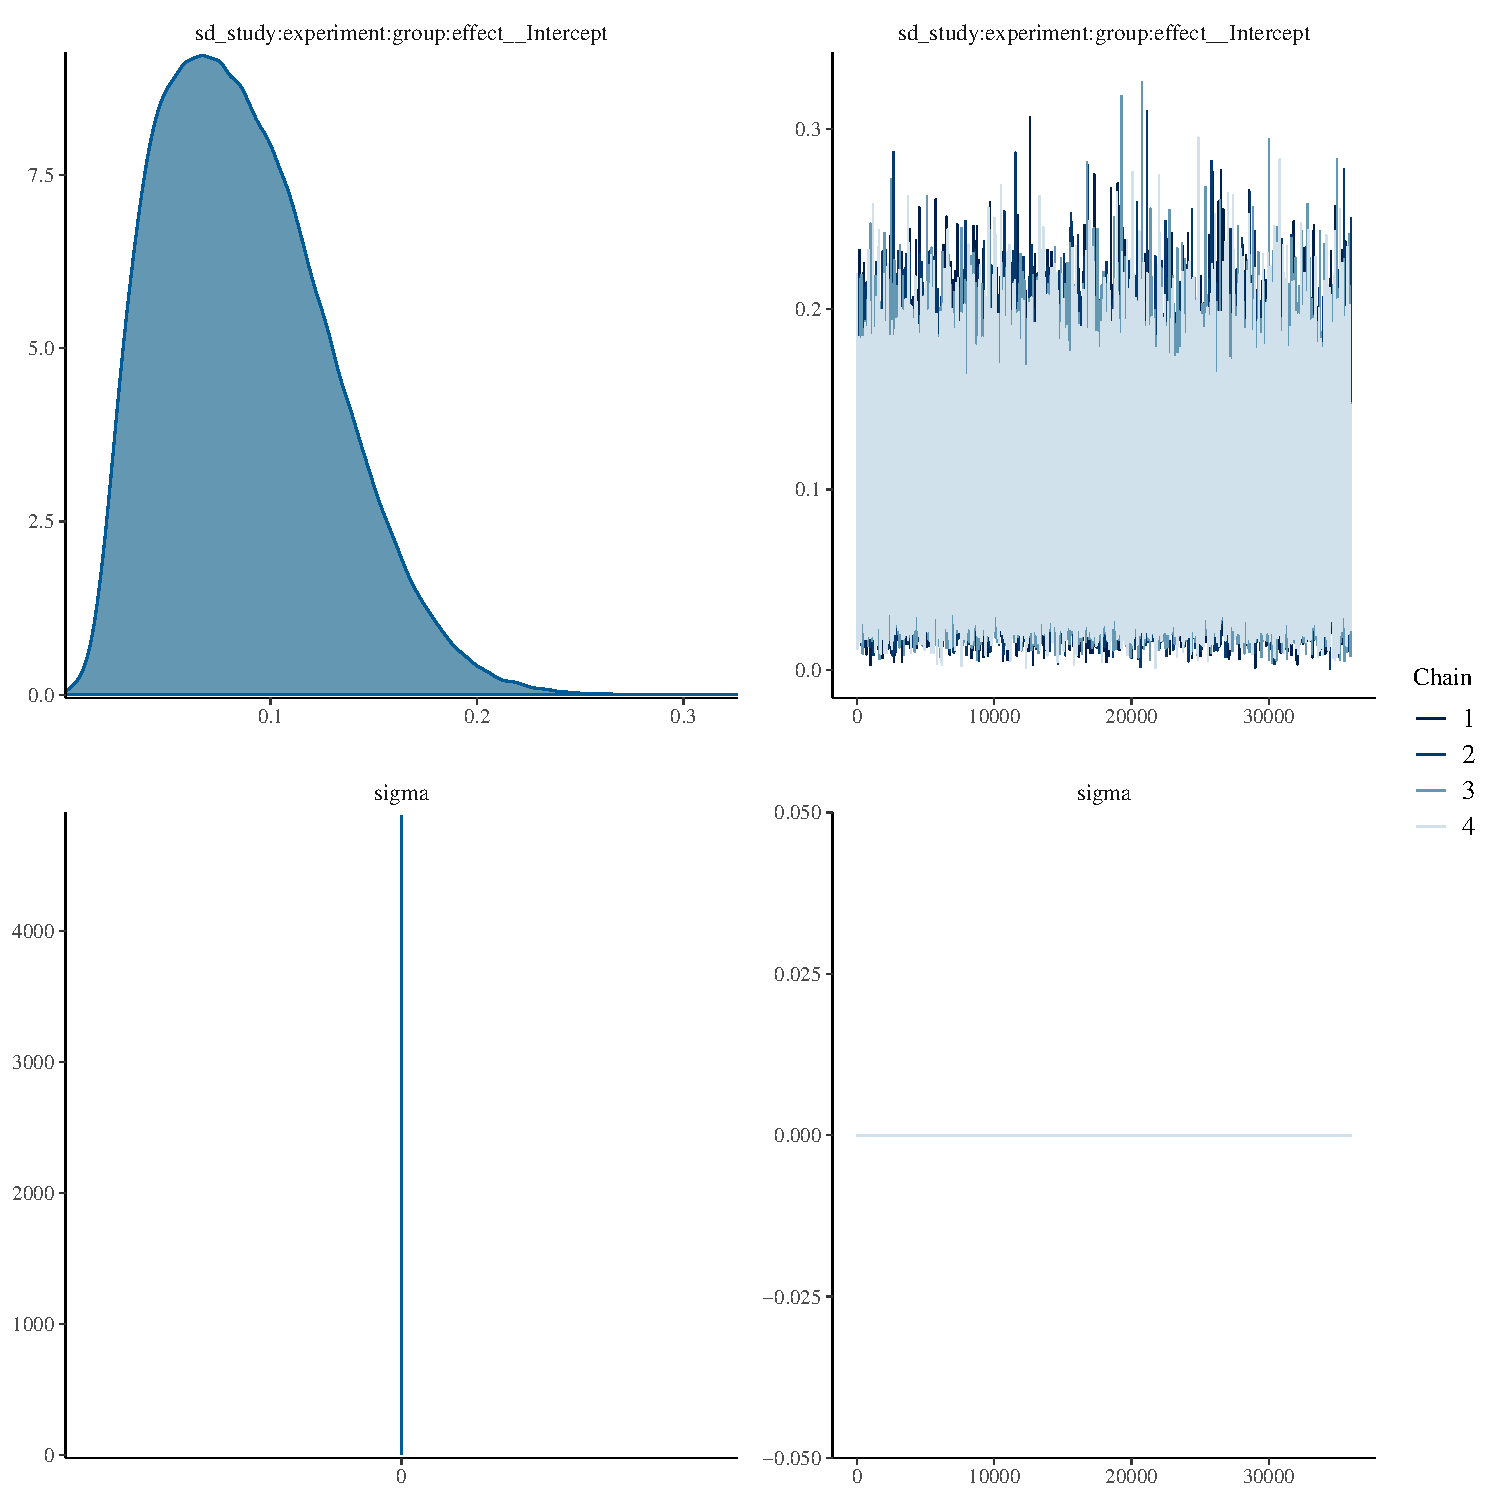
\includegraphics[width=1\textwidth,height=\textheight]{diagnostic_plots_files/figure-pdf/unnamed-chunk-23-2.pdf}

}

\end{figure}

\begin{verbatim}
[[1]]

[[2]]
\end{verbatim}

\hypertarget{posterior-predictive-check-7}{%
\section{Posterior predictive
check}\label{posterior-predictive-check-7}}

\begin{figure}

{\centering 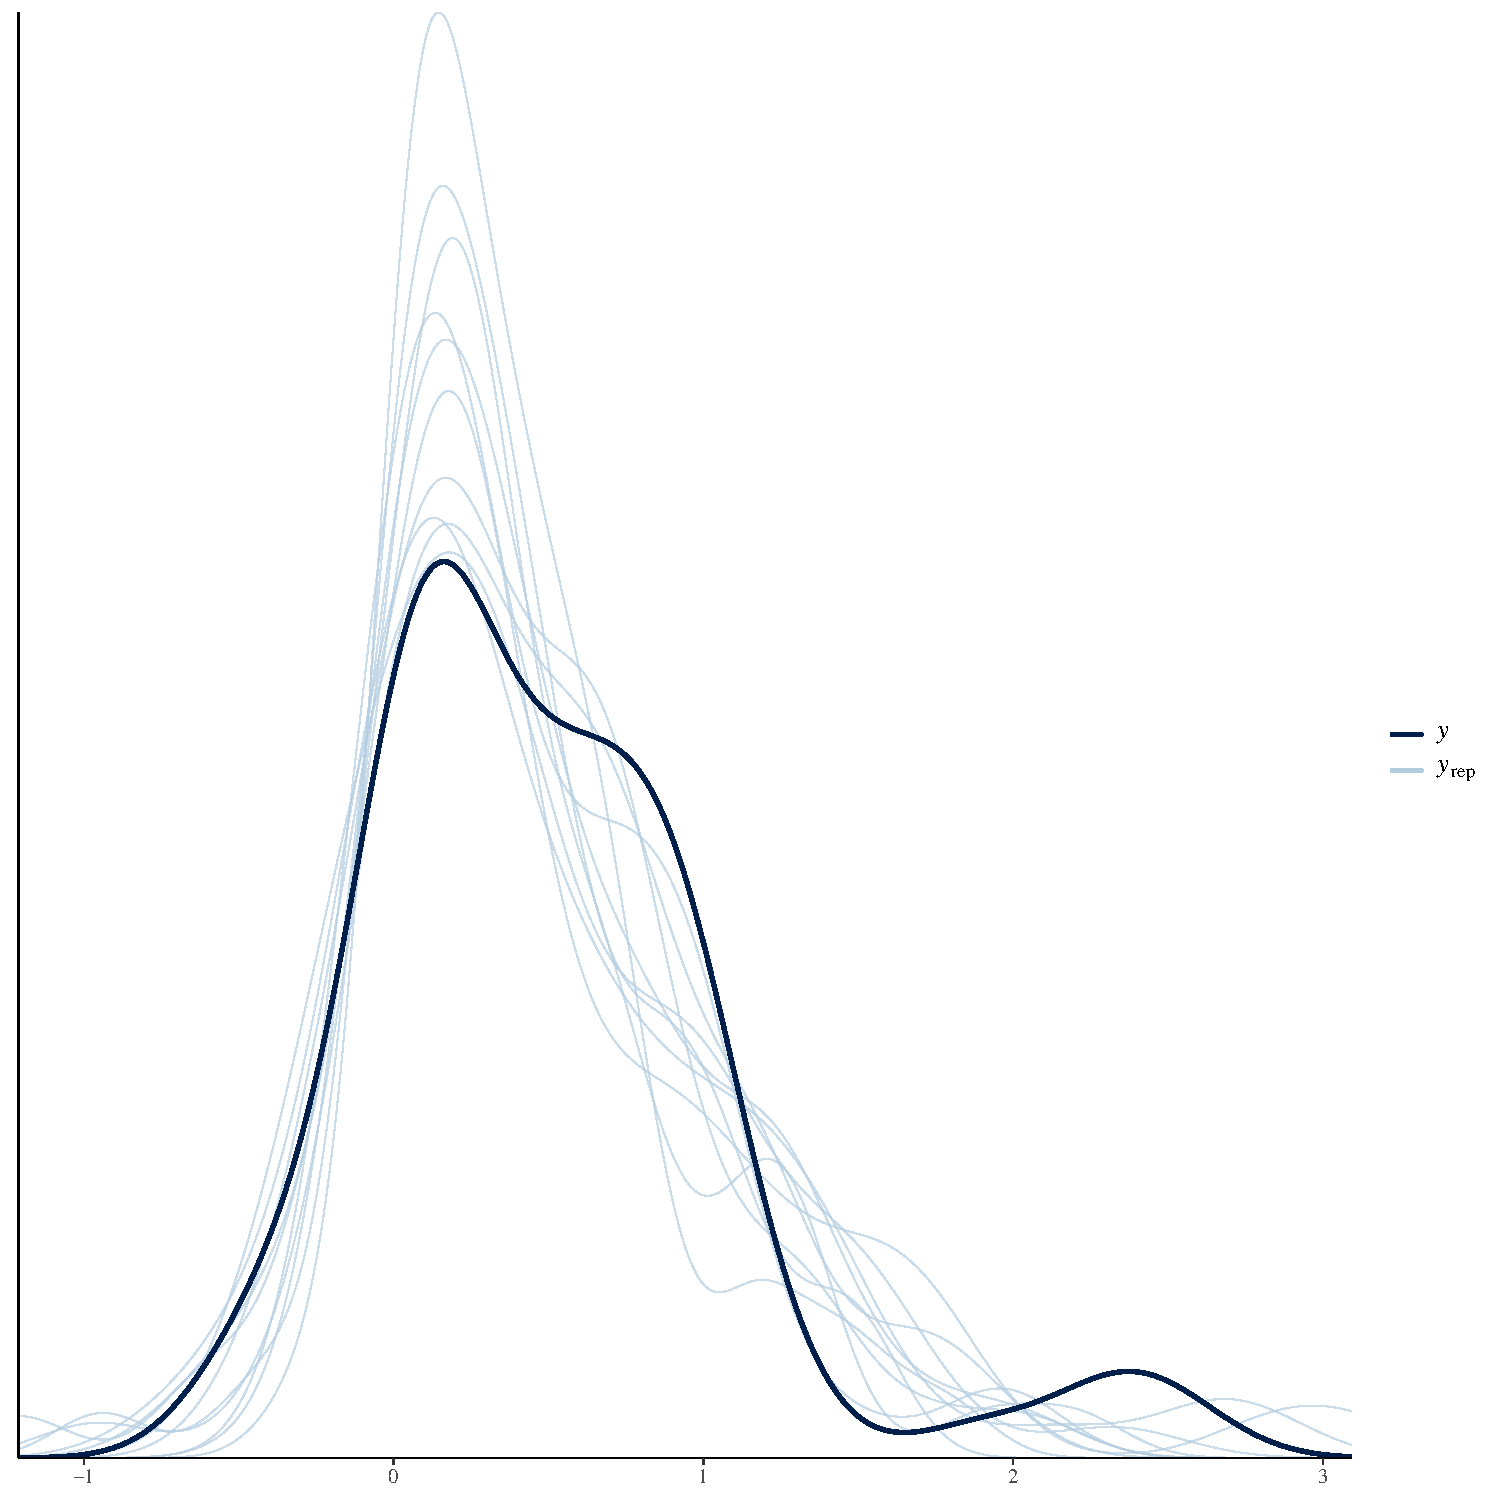
\includegraphics[width=1\textwidth,height=\textheight]{diagnostic_plots_files/figure-pdf/unnamed-chunk-24-1.pdf}

}

\end{figure}

\hypertarget{training-model}{%
\chapter{Training Model}\label{training-model}}

\hypertarget{hatr-8}{%
\section{\texorpdfstring{\(\hat{R}\)}{\textbackslash hat\{R\}}}\label{hatr-8}}

\begin{figure}

{\centering 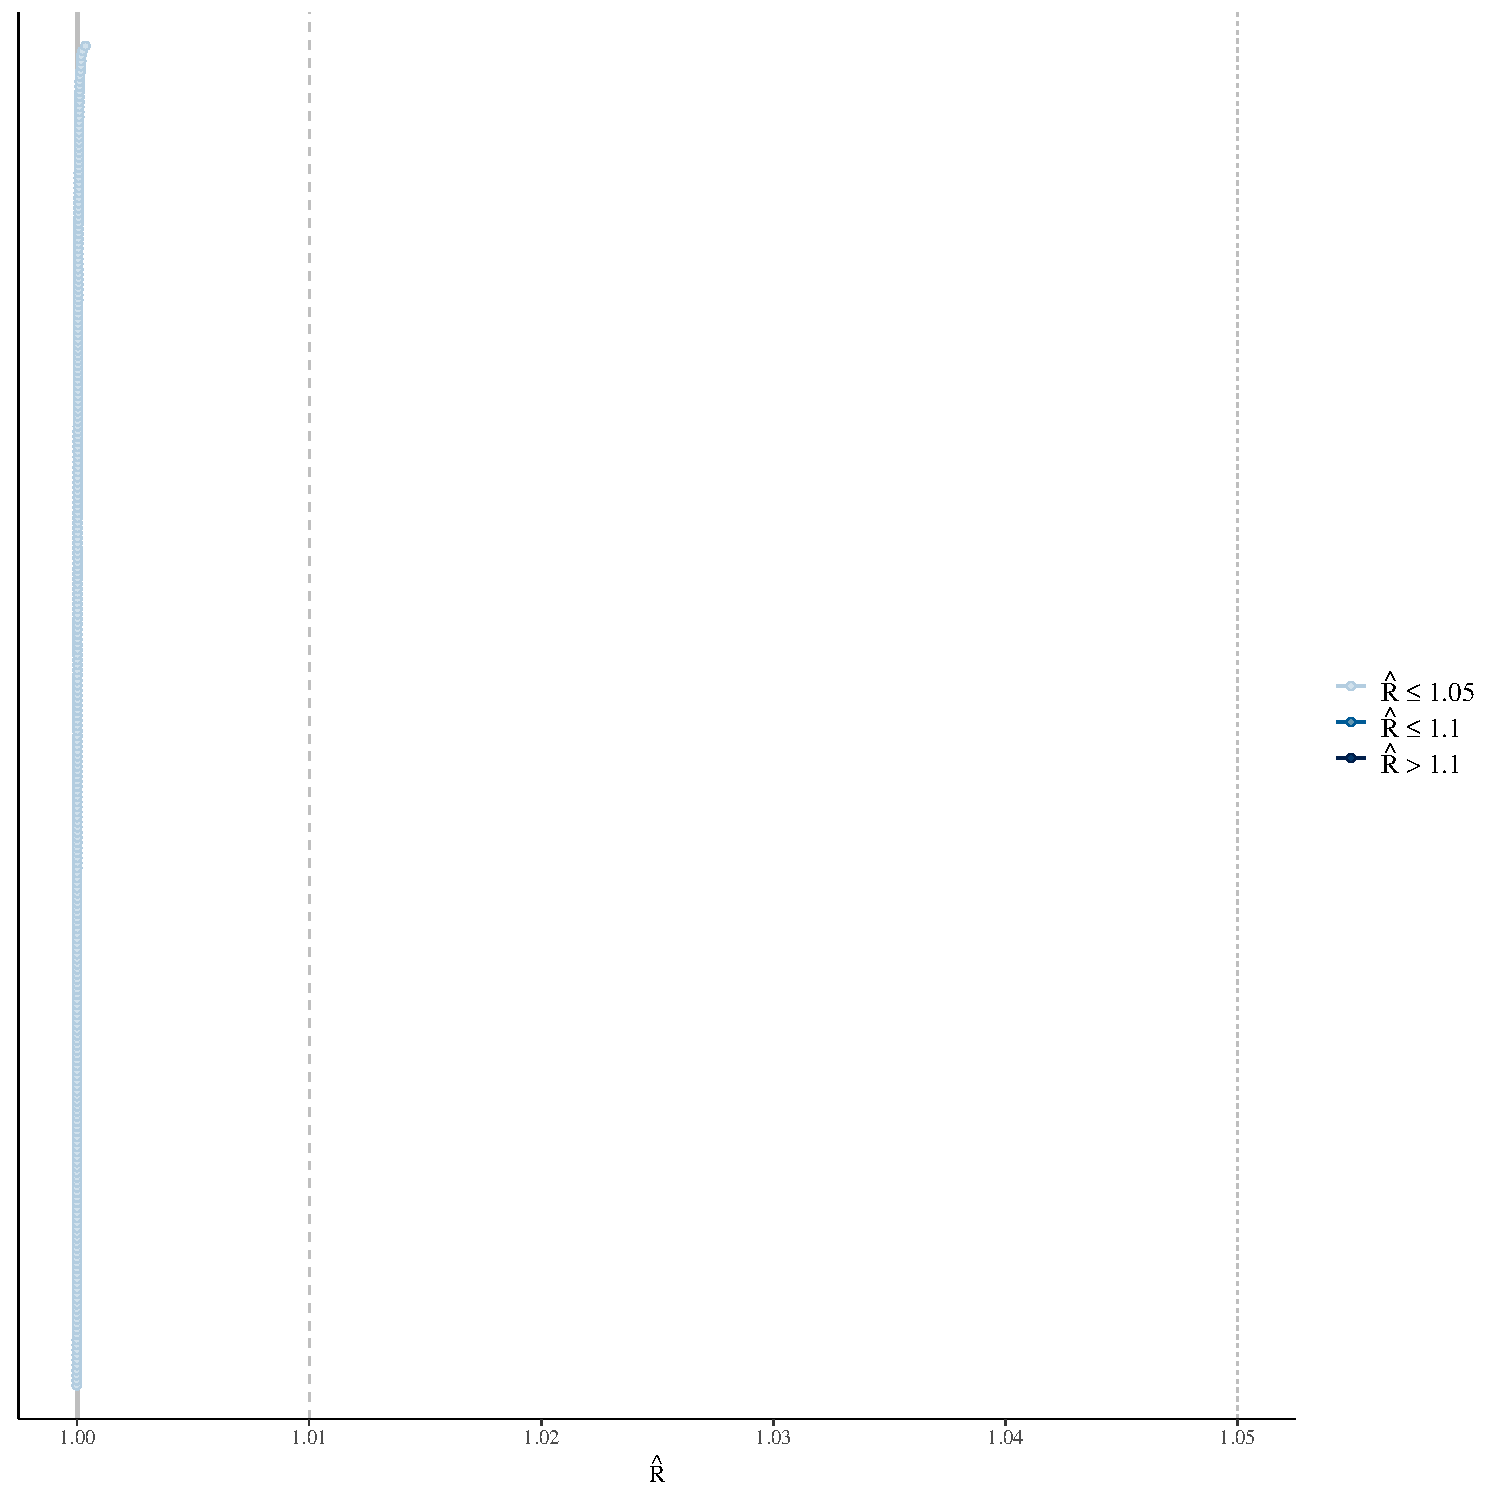
\includegraphics[width=1\textwidth,height=\textheight]{diagnostic_plots_files/figure-pdf/unnamed-chunk-25-1.pdf}

}

\end{figure}

\hypertarget{trace-plots-8}{%
\section{Trace plots}\label{trace-plots-8}}

\begin{figure}

{\centering 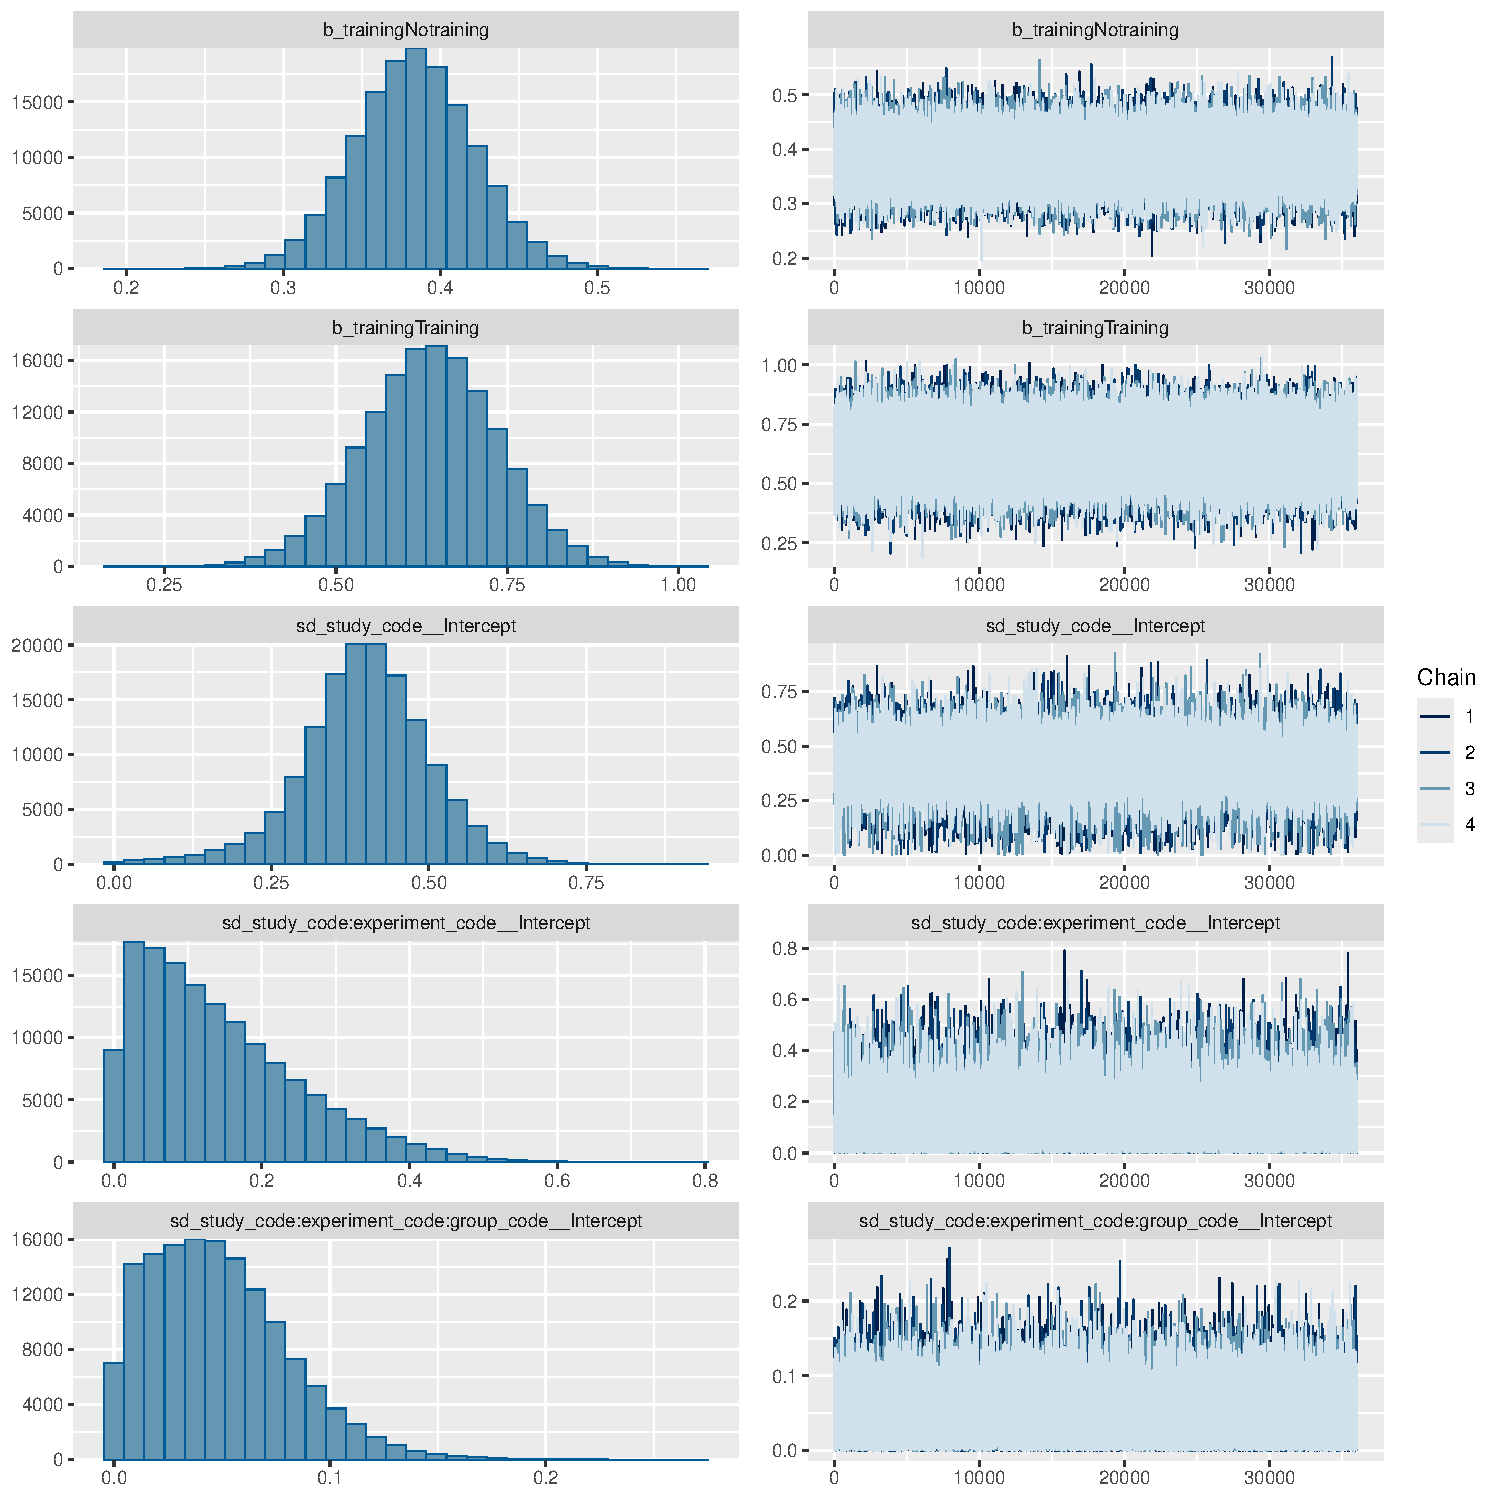
\includegraphics[width=1\textwidth,height=\textheight]{diagnostic_plots_files/figure-pdf/unnamed-chunk-26-1.pdf}

}

\end{figure}

\begin{figure}

{\centering 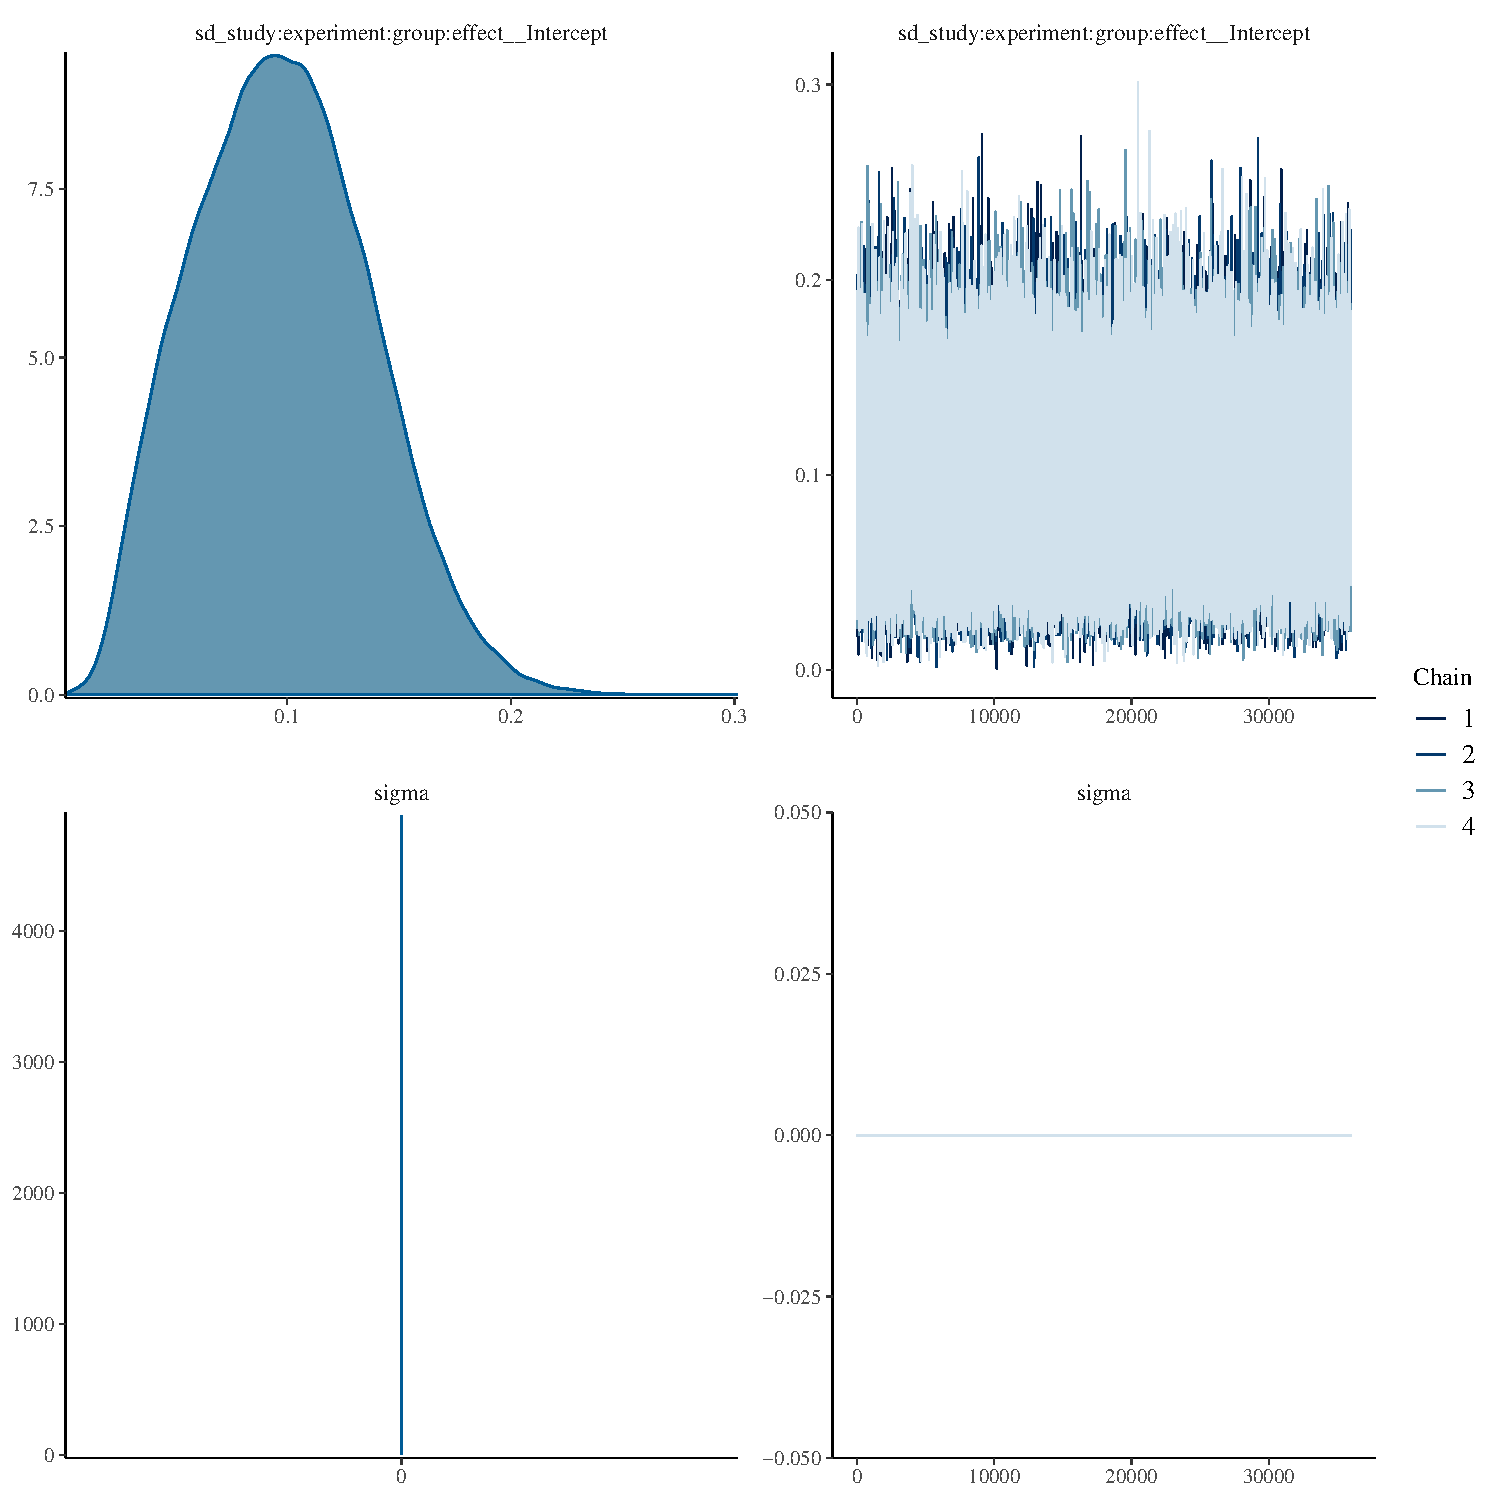
\includegraphics[width=1\textwidth,height=\textheight]{diagnostic_plots_files/figure-pdf/unnamed-chunk-26-2.pdf}

}

\end{figure}

\begin{verbatim}
[[1]]

[[2]]
\end{verbatim}

\hypertarget{posterior-predictive-check-8}{%
\section{Posterior predictive
check}\label{posterior-predictive-check-8}}

\begin{figure}

{\centering 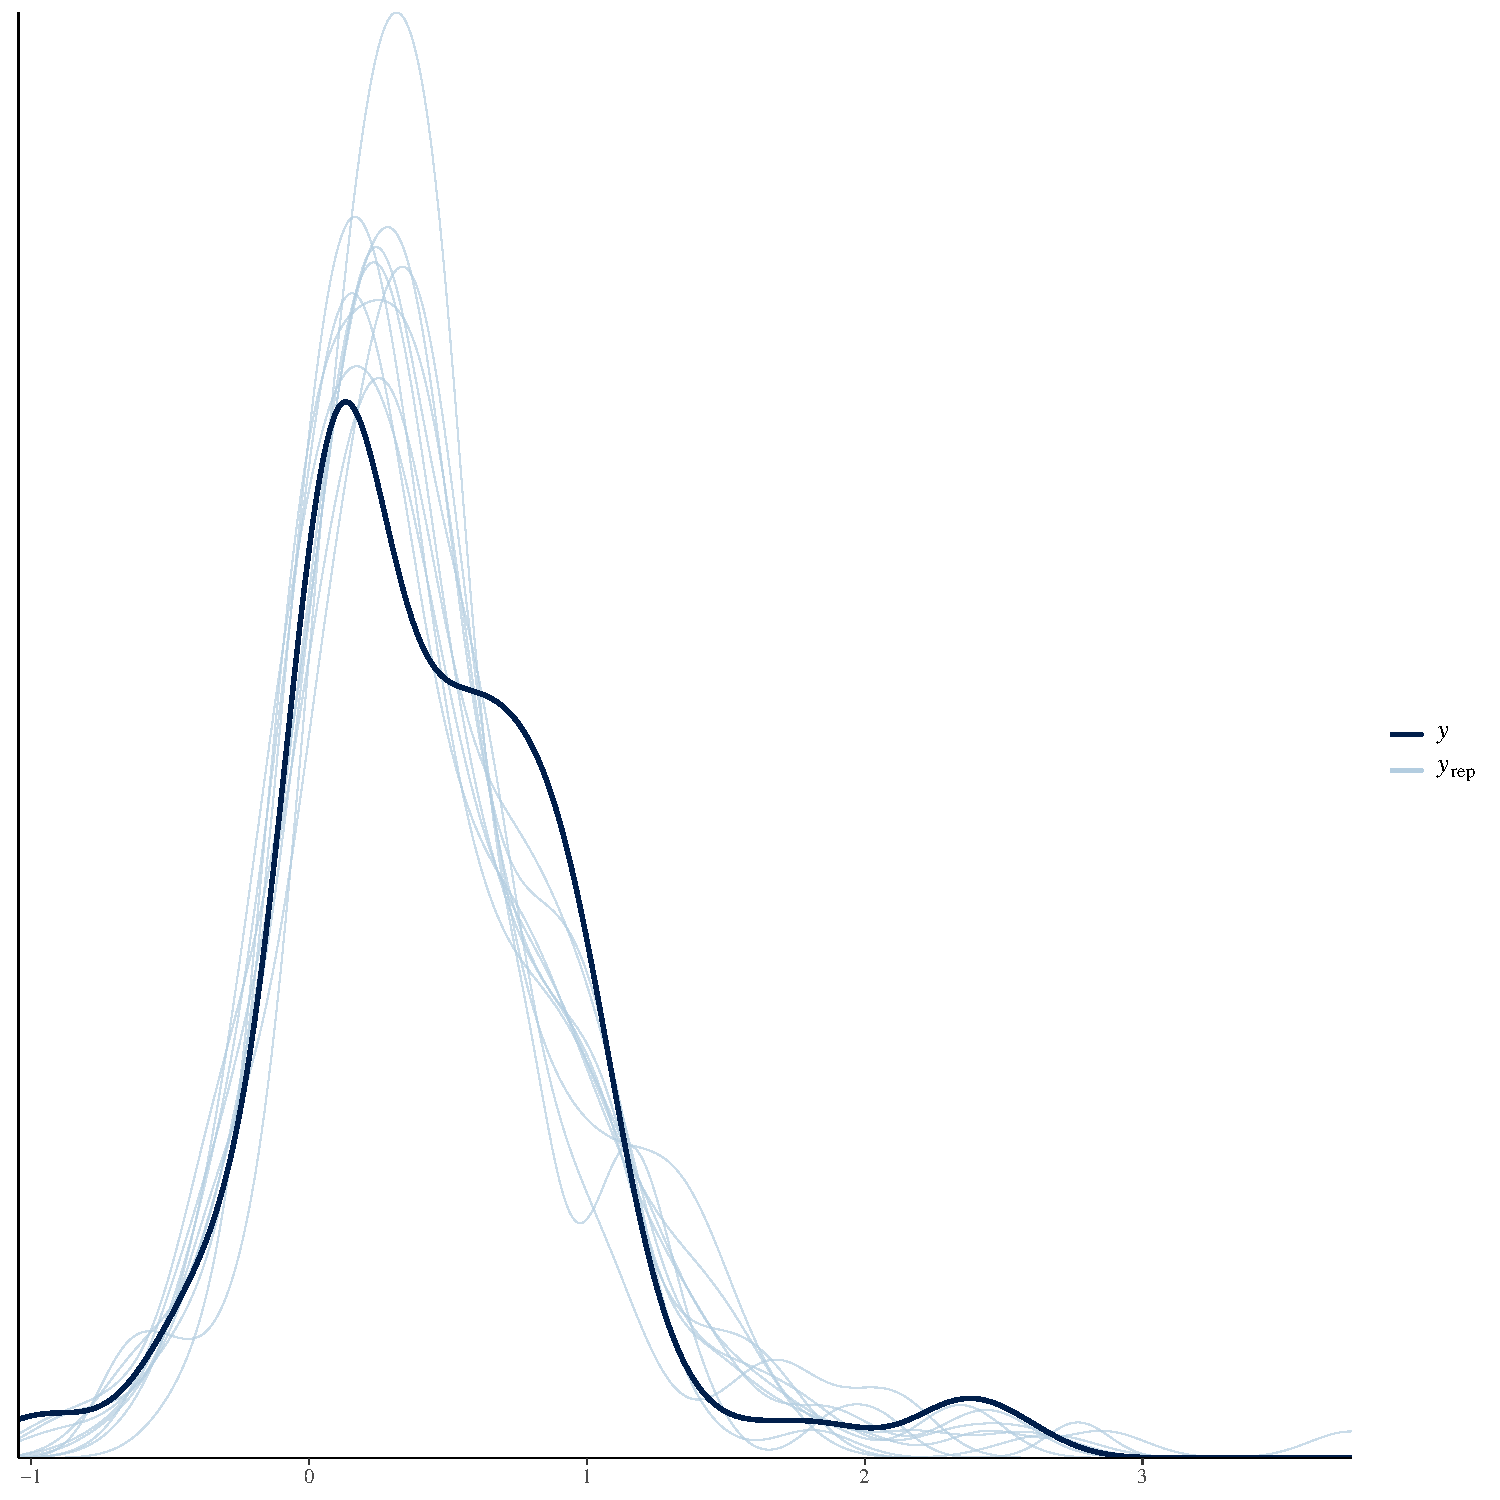
\includegraphics[width=1\textwidth,height=\textheight]{diagnostic_plots_files/figure-pdf/unnamed-chunk-27-1.pdf}

}

\end{figure}

\hypertarget{study-design-model}{%
\chapter{Study Design Model}\label{study-design-model}}

\hypertarget{hatr-9}{%
\section{\texorpdfstring{\(\hat{R}\)}{\textbackslash hat\{R\}}}\label{hatr-9}}

\begin{figure}

{\centering 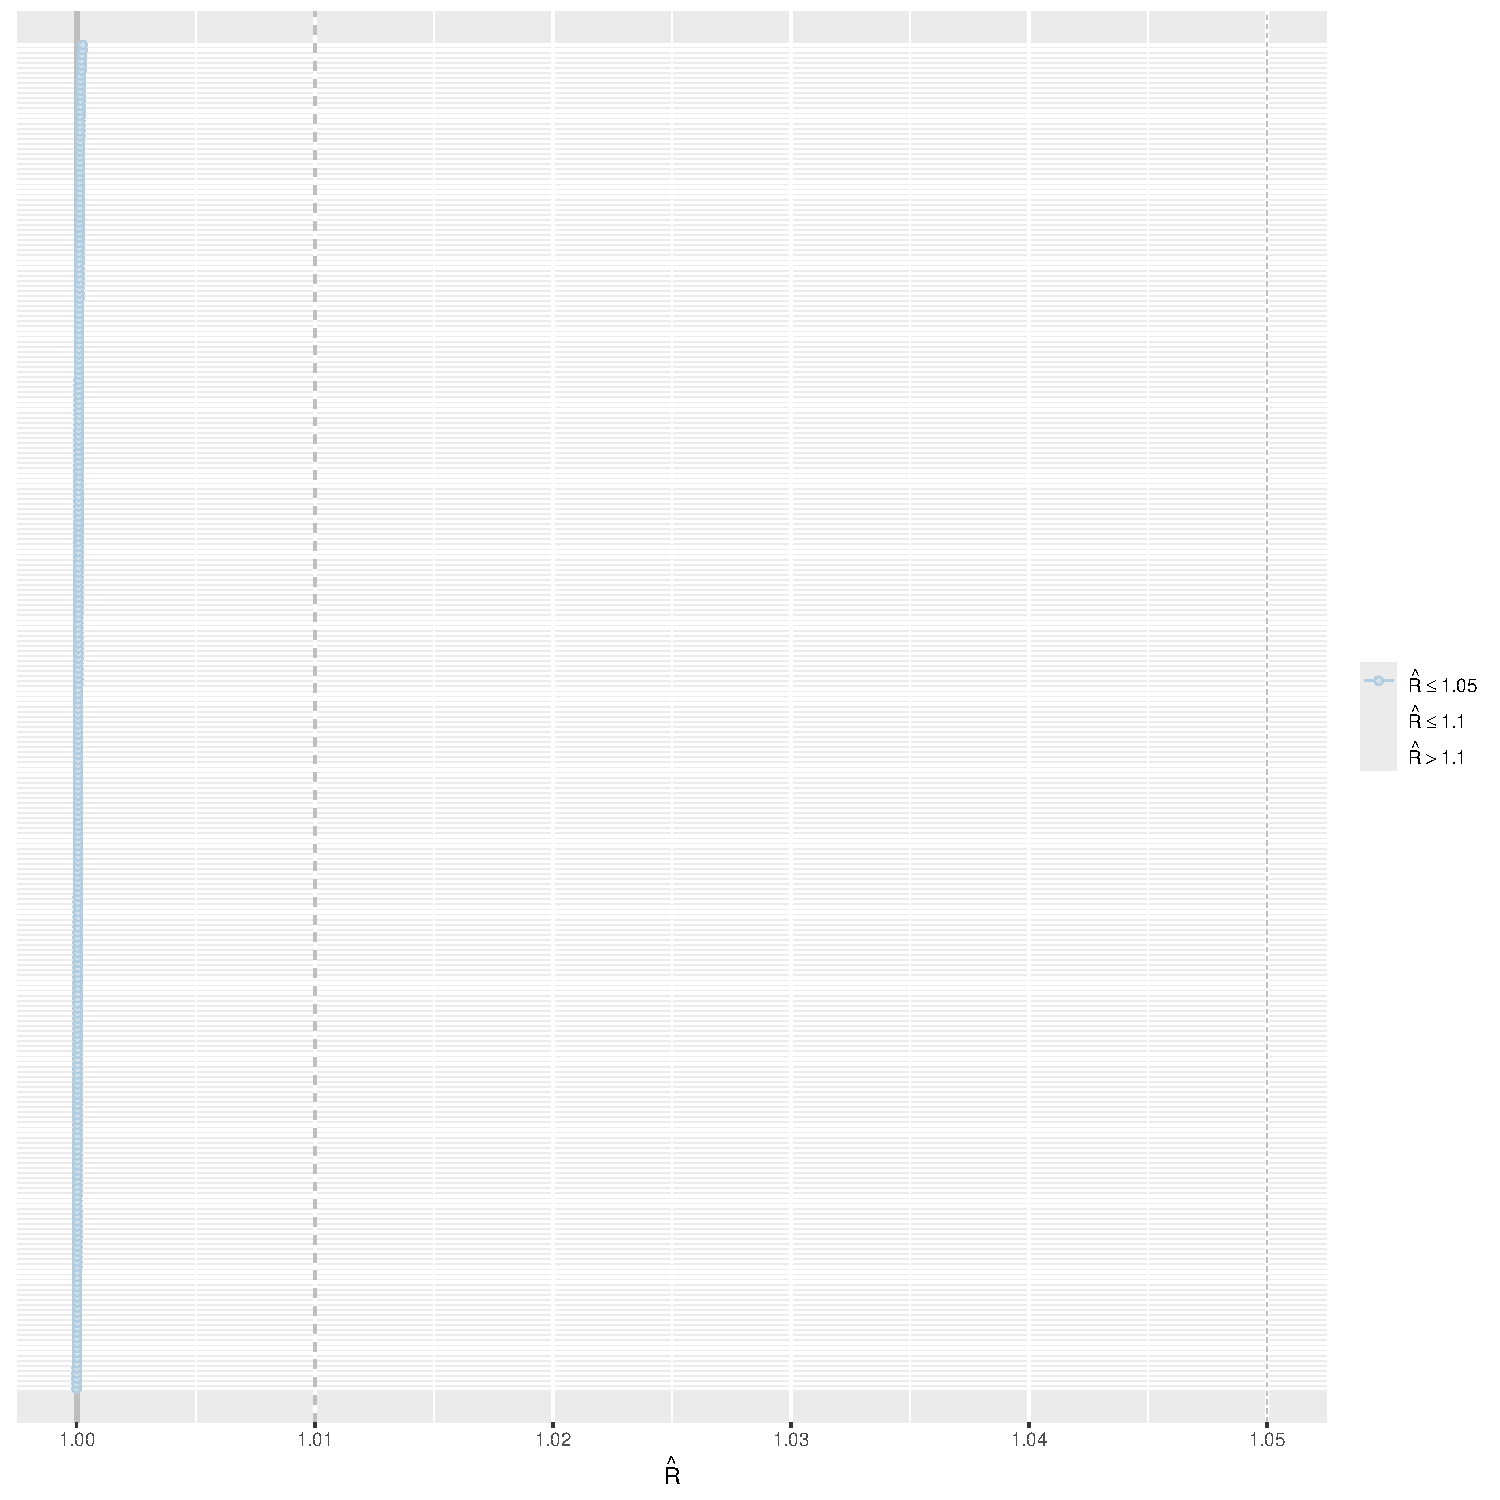
\includegraphics[width=1\textwidth,height=\textheight]{diagnostic_plots_files/figure-pdf/unnamed-chunk-28-1.pdf}

}

\end{figure}

\hypertarget{trace-plots-9}{%
\section{Trace plots}\label{trace-plots-9}}

\begin{figure}

{\centering 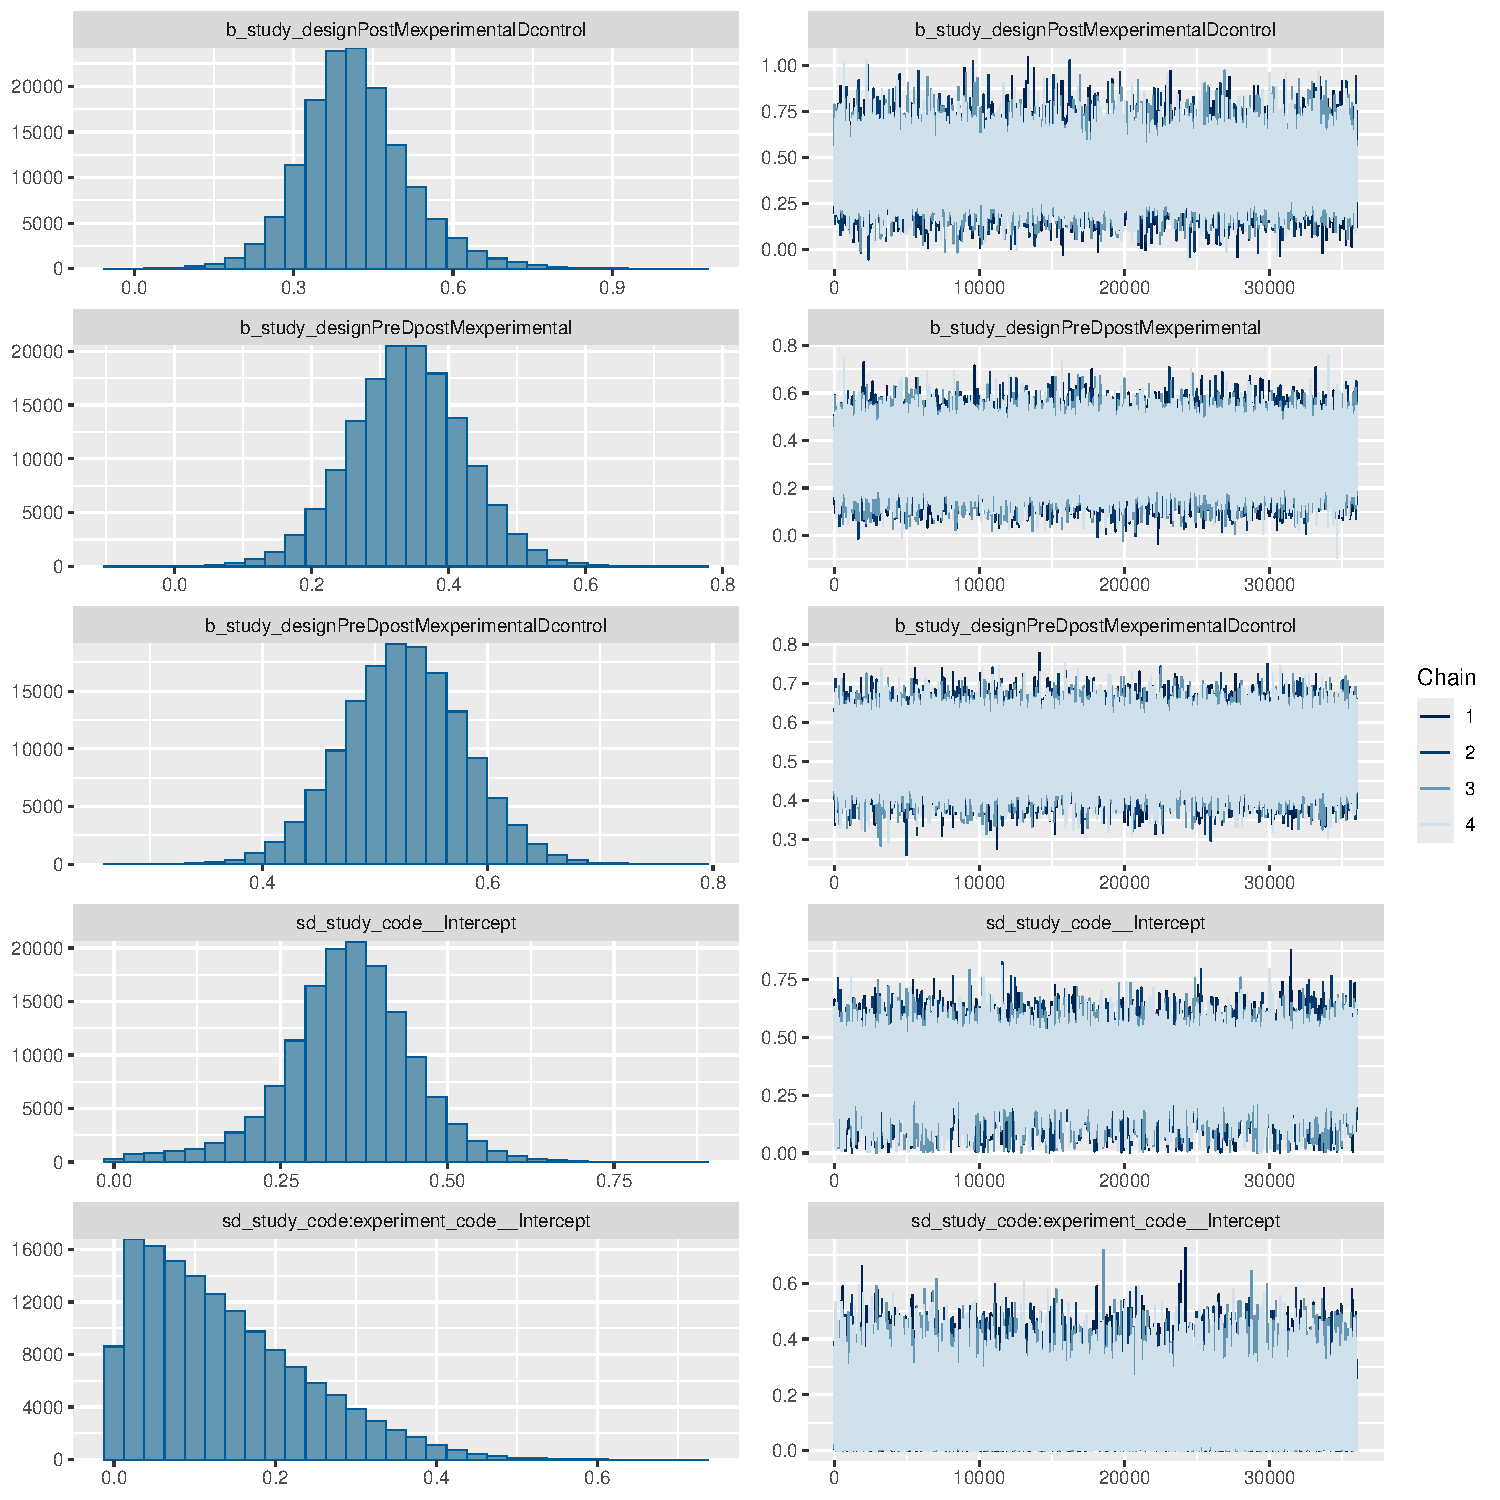
\includegraphics[width=1\textwidth,height=\textheight]{diagnostic_plots_files/figure-pdf/unnamed-chunk-29-1.pdf}

}

\end{figure}

\begin{figure}

{\centering 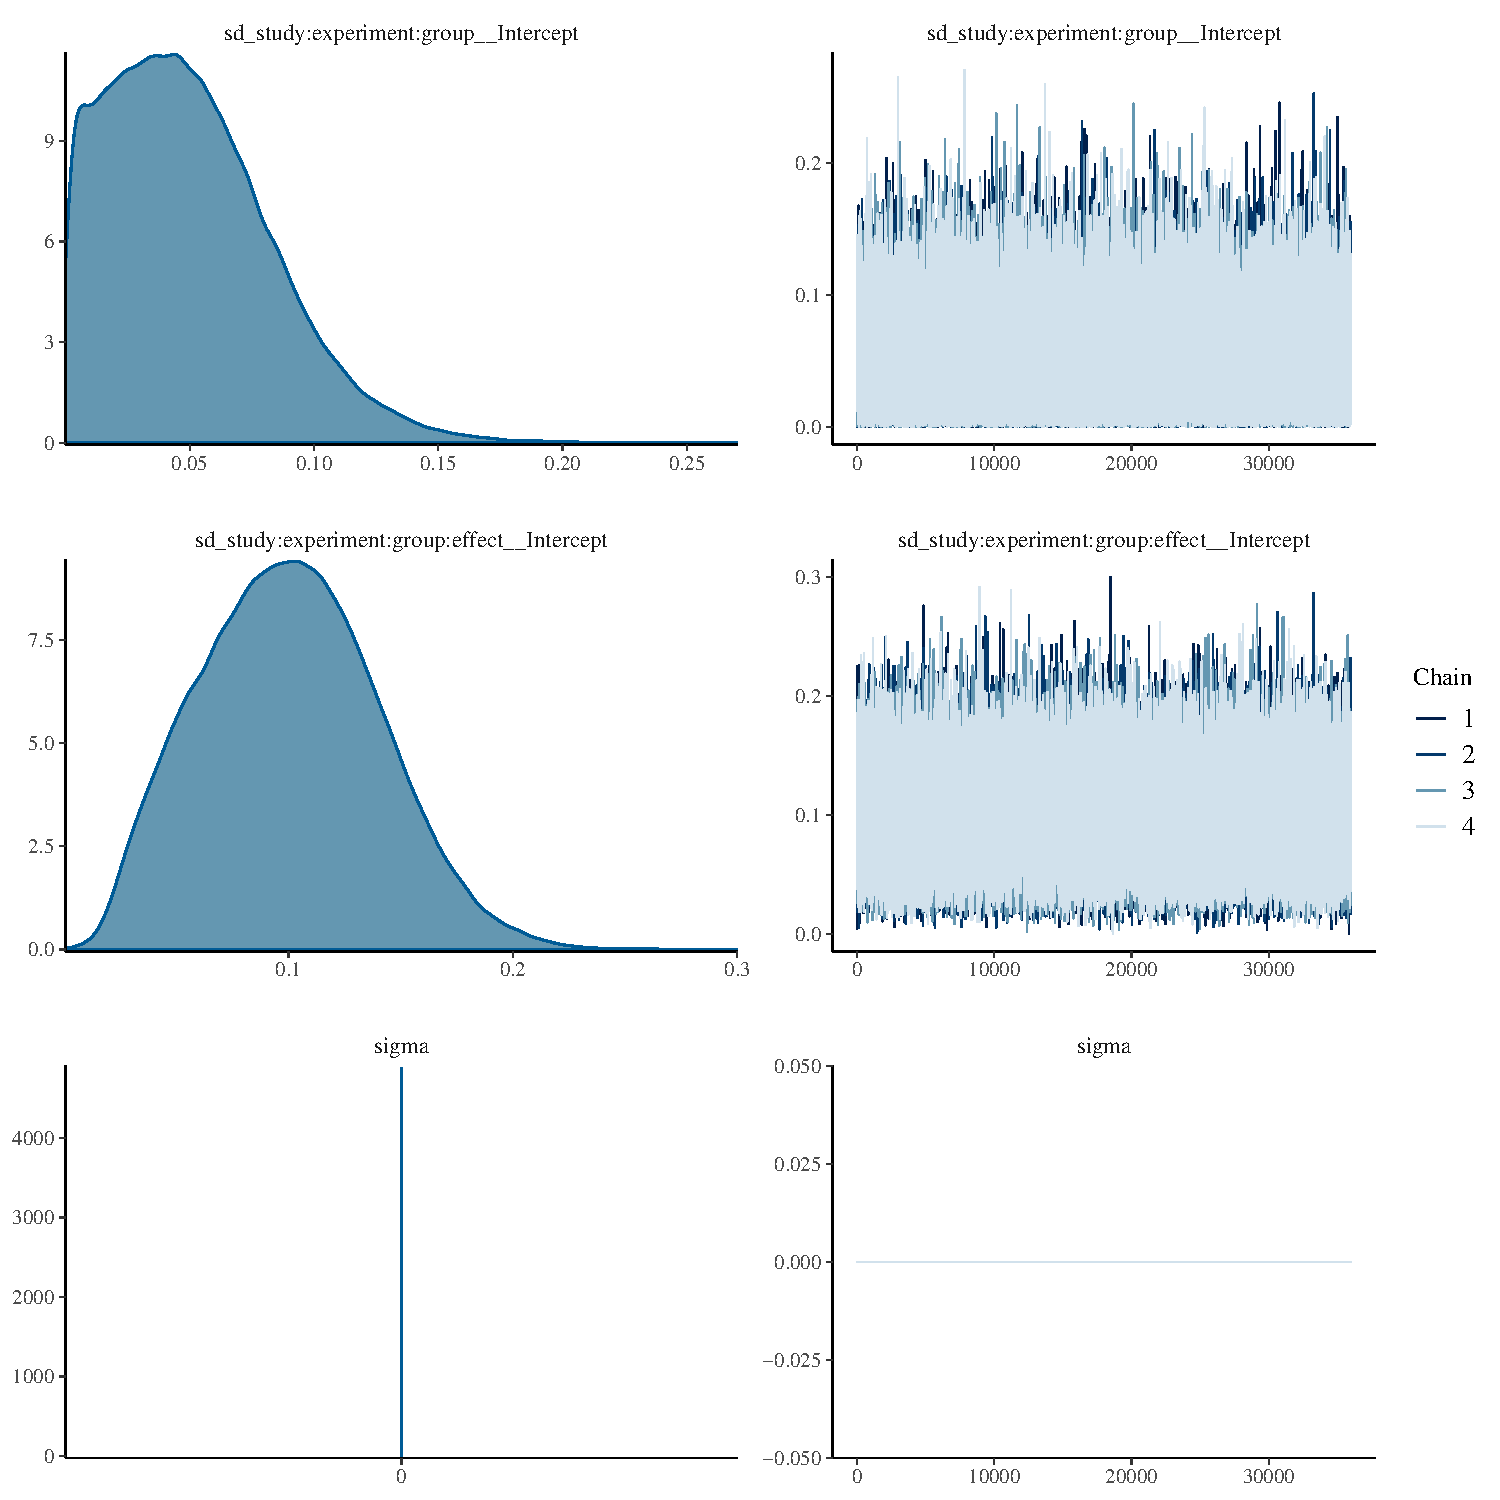
\includegraphics[width=1\textwidth,height=\textheight]{diagnostic_plots_files/figure-pdf/unnamed-chunk-29-2.pdf}

}

\end{figure}

\begin{verbatim}
[[1]]

[[2]]
\end{verbatim}

\hypertarget{posterior-predictive-check-9}{%
\section{Posterior predictive
check}\label{posterior-predictive-check-9}}

\begin{figure}

{\centering 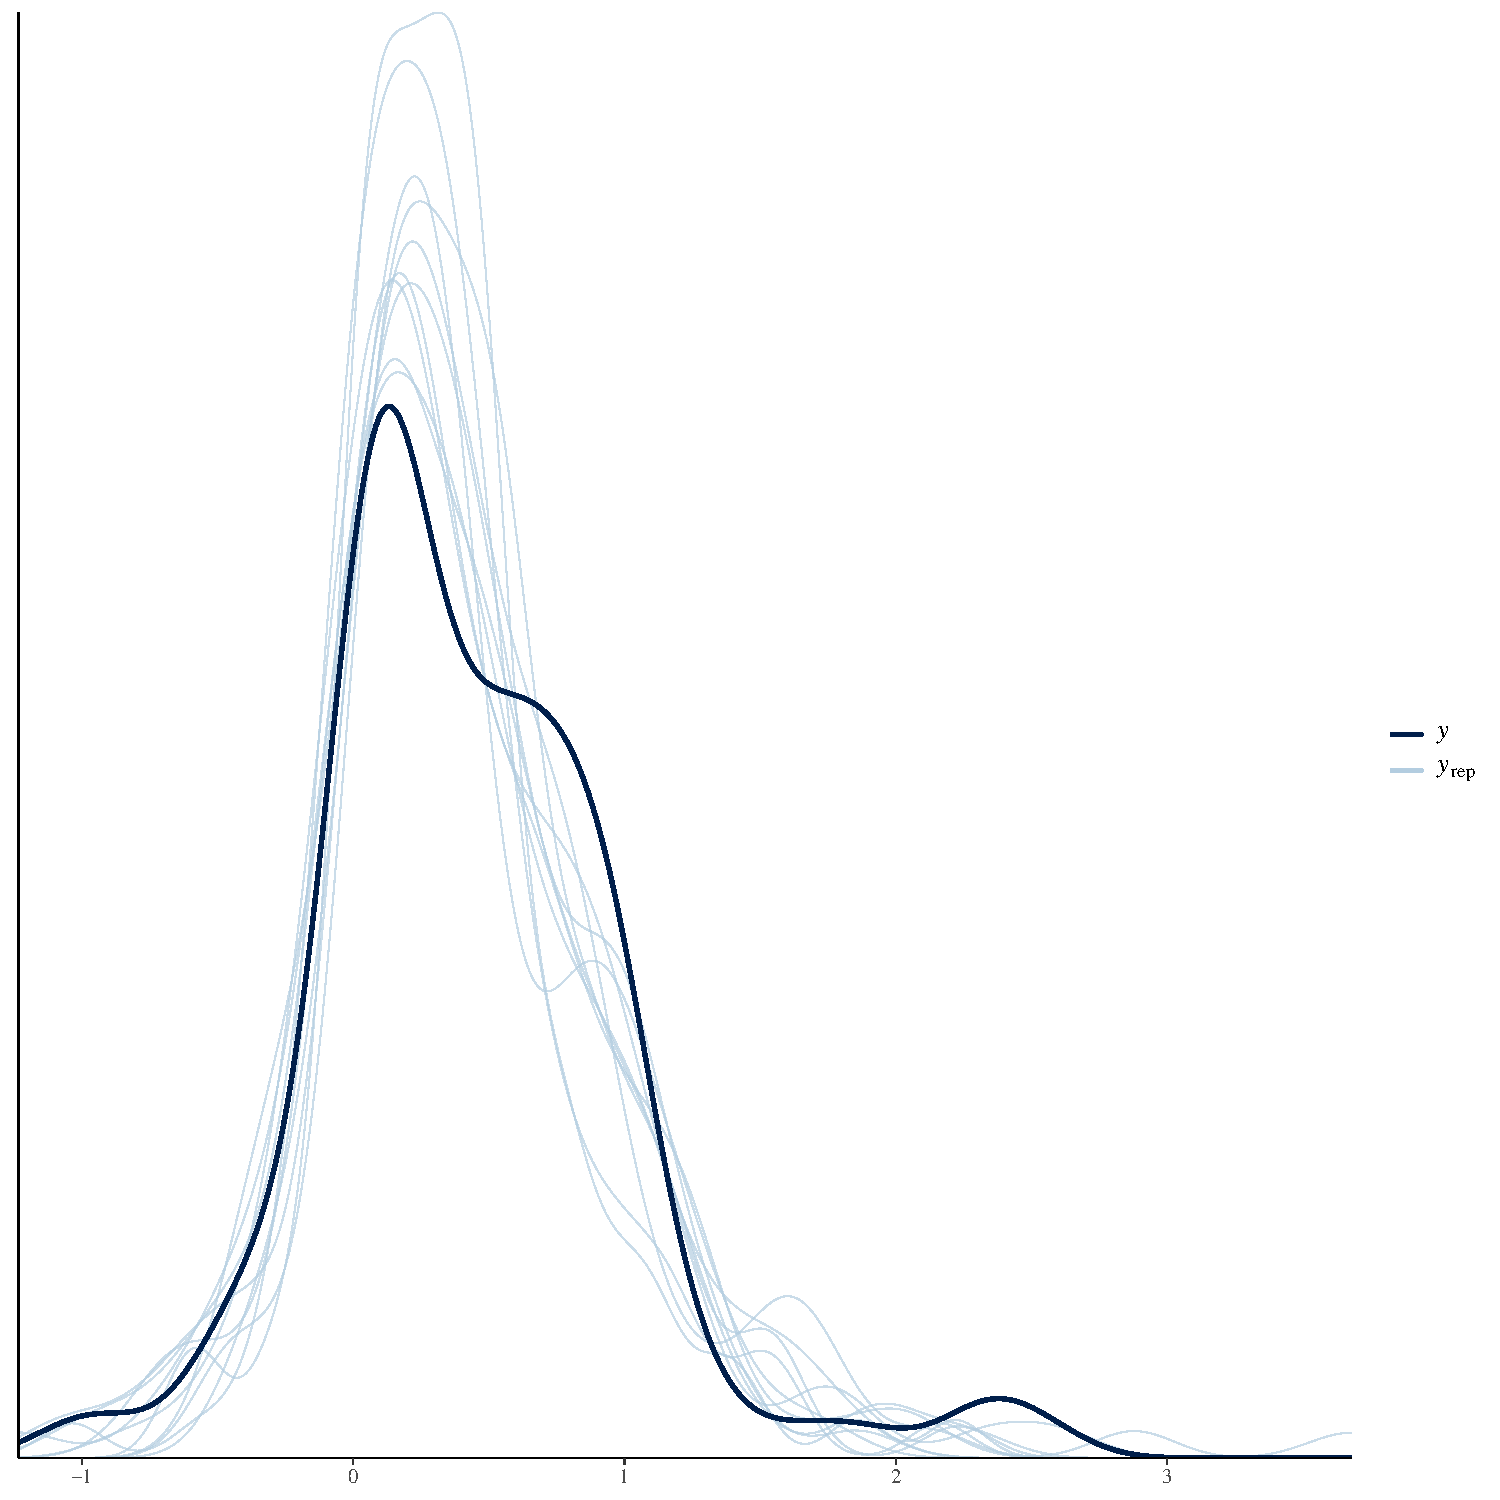
\includegraphics[width=1\textwidth,height=\textheight]{diagnostic_plots_files/figure-pdf/unnamed-chunk-30-1.pdf}

}

\end{figure}



\end{document}
